%% Before beginning to type your dissertation, read the formatting guide, 
%% which can be found at http://grad.msu.edu/etd/docs/formattingguide.pdf
%% Also get the latest version of  msuphddissertation.cls and the template file
%% at http://www.math.msu.edu/~weil/MSU_Ph.D._Dissertation.zip
%% Send questions to weil@math.msu.edu
\documentclass{msuphddissertation}
\usepackage{amssymb, amsmath}
%\usepackage{subcaption}
\usepackage{graphicx}
\usepackage{rotating}
\usepackage{url}
%% Insert packages you wish to use except setspace and subfig. 
%% Those packages are loaded automatically.
%% IMPORTANT: Load only those packages you know you will use.
%% Some packages can cause conflicts resulting in improper formatting.
\author{Qingpeng Zhang} %% Put your name in full as it is officially recognized by Michigan State University here.
\title{Novel Computational Approaches to Investigate Microbial Diversity} %% Put the title of your dissertation here.
\unit{Computer Science} %% Put the name of your degree granting unit here. The complete
%% list of these degree granting units can be found at
%% http://grad.msu.edu/etd/docs/DegreeGrantingUnits.pdf

%% Put additional preamble items here.

%%%%%% LANDSCAPE PAGES  %%%%%%
%% The environment, landscapenum, produces a page in 
%% landscape mode and then rotates the page by 90 degrees 
%% making is readable on a computer screen, and places the page number
%% along the 11 inch side, which is the bottom of the rotated page. 

%%%%%%%%%%%%%%%%%%%%%%%%%%%%
%%%%%%%%  NOTE   %%%%%%%%%%%%%%
%% PREPARING A DISSERTATION WITH THIS CLASS FILE DOES NOT %%%
%% GUARANTEE THAT THE GRADUATE SCHOOL WILL APPROVE IT %%%
%%%%%%%%%%%%%%%%%%%%%%%%%%%%%%%

%%%%%%%%%%%%%%%%%%%%%%%%%%%%%%%%%%
%%%%%%%%%%%% WARNING %%%%%%%%%%%%%%%
%% The Graduate School requires that all text, except superscripts %%
%% and subscripts, but including text in imported %%
%% graphics files be in 12 point. For that reason it's recommended %%
%% that no text be part of any imported files. %%

%% Once your document has been filed with the Graduate School,
%% if you wish to produce a version of it whose subscripts and superscripts
%% are in traditional smaller proportion, remove the "%" sign 
%% in front of following command. 
%\DeclareMathSizes{12}{12}{10}{8}
%% If your document has footnotes, remove the "%" sign 
%% in front of following command. 
%\renewcommand{\footnotesize}{\small}
%% To single space your document, remove the 
%% two commands \begin{doublespace}
%% and \end{doublespace} below.

\begin{document}

\maketitlepage %%This command will produce the title page of your thesis.
\begin{abstract}



 Species diversity is an important measurement of ecological communities. Scientists 
believe that there is a strong relationship between species diversity and ecosystem processes.
 In almost all metagenomics projects, diversity analysis plays an important role in supplying information 
 about the richness of species, the species abundance
distribution in a sample, and the similarity/difference between 
samples, all of which are crucial to draw insightful and reliable conclusions. Since we have limited
 sequencing power and financial constraints, the metagenomics data sets from 
 high diversity samples like soil only correspond to a tiny fraction of the actual genomic
 content in the sample. The large size of data sets and low coverage make the assessment of microbial 
 diversity in complex samples even harder. With novel applications of data structures and the development 
 of novel algorithms, my research provides the necessary and highly desired computational methods to enable 
 scalable microbial diversity analysis of the complex metagenomes, with further potential to facilitate other analysis like assembly, annotation.


 This dissertation
covers an overview of existing approaches of doing microbial diversity analysis
 of metagenomic samples, especially based on the concept of OTU, including the
steps in the procedure, like contigs binning, statistical
analysis of OTU abundance information to estimate the microbial diversity.  As
the foundation of the IGS based framework, we described a novel method to count k-mers
efficiently and a scalable approach to retrieve the coverage of a read in a 
data set based on efficient and online k-mer counting. We also introduced the
applications of this approach in reducing the redundancy of metagenomic reads
dataset and analyzing sequencing error, which is beneficial to other tasks 
in metagenomic data analysis, like
assembly or error trimming. Next, we discussed how we developed the concept 
of IGS based on the methods of efficient k-mer counting and digital
normalization discussed before.  
The application of IGS to analyze microbial diversity of metagenomic data sets 
was discussed and the performance of the IGS method on simulated data sets and
real data sets were demonstrated in the final chapters. 
Since this method is totally binning-free,
assembly-free, annotation-free, reference-free, it is specifically promising to
deal with the highly diverse samples, while we are facing large amount of dark
matters in it, like soil.

  



\end{abstract}

%% If you wish to have a copyright page, remove the "%" in front of  \begin{copyrt}
%% and remove the "%" in front of \end{copyrt}.
%% The mandatory form of the Copyright will be generated automatically. 
%% A copyright statement is optional.

%\begin{copyrt}
%\end{copyrt}
%% If you wish to have a dedication, remove the "%" in front of
%% \begin{dedication}
%% \end{dedication}
%% A dedication must be single-spaced and 
%% centered on the page.  Both will be done automatically. 

\begin{dedication}
\begin{center} 
Dedication goes here.
\end{center}
\end{dedication}

%% If you wish to have an acknowledgment, remove the "%" in front of  \begin{acknowledgment}
%% and remove the "%" in front of  \end{acknowledgment}  
\begin{acknowledgment}
Acknowledgements go here

\end{acknowledgment}

%% If you wish to have a preface, remove the "%" in front of  \begin{preface}
%% and remove the "%" in front of  \end{preface}  
%\begin{preface}
%% Type your acknowledgment here. An acknowledgment is optional.
%\end{preface}

\TOC

%% If your document contains tables, remove the "%" in front of 
%%  the following line.
\LOT

%% If your document contains figures, remove the "%" in front of
%% the following line.
\LOF

%% If any of your figures contain color, you must
%% include the following disclaimer in the caption of your first figure.
%% "For interpretation of the references to color in this and all other figures, 
%% the reader is referred to the electronic version of this dissertation."

%%%% LIST OF SYMBOLS AND ABBREVIATIONS %%%%
%% Such a list is possible using the environment
%% abbreviationskey
%% here. The list will be included in the TOC as
%% KEY TO SYMBOLS AND ABBREVIATIONS
%%%%%%%%%%

\newpage
\pagenumbering{arabic}
\begin{doublespace}

%% Put the body of your dissertation here. 
%% DO NOT include  the bibliography

\chapter{Introduction}

\section{Overview} Species diversity is an important measurement of ecological
communities. Scientists believe that there is a relationship between species
diversity and ecosystem processes \cite{Loreau:2001aa}. Evaluating the species
diversity in a community is a central research topic in macroorganism ecology.
Many methods have been developed over the last few decades, aimed at answering
questions such as ``how many species of birds are in this habitat''.
Nevertheless, until recently scientists had not started to think seriously
about larger-scale questions such as ``How many species are there on earth?''
\cite{May:1988aa} or ``How many species are there in the ocean?''
\cite{Mora:2011aa} until recently. Why? The answer is straightforward:
Microorganisms represent the vast majority of the Earth's biodiversity and the
assessment of microbial diversity is quite difficult.

It is believed that microbial diversity is the outermost frontier of the
exploration of diversity \cite{magurran2011biological}. Microorganisms are
ubiquitous. They were the first forms of life on the Earth. There are more
bacterial cells in our body than human cells \cite{Savage:1977aa}. 
There are several reasons why assessment of microbial diversity is such a
challenge. First, the concept of species is ambiguous. Morphological
examination is impossible: fewer than 1\% of microorganisms  in the biosphere
can not be cultivated by traditional cultivation
techniques\cite{Curtis:2002aa}. To overcome this obstacle, metagenomics has
emerged, driven by the progress of next-generation sequencing (NGS) technology.
Lots of metagenomics projects have been performed on samples ranging from acid
mine drainage channels to human gut. For complex environmental samples such as
soil, the resulting data sets can be huge. There are approximately a billion
microbial cells, with about 4 petabase pairs of DNA($4*{10}^{12}$ bp)
\cite{Zarraonaindia:2013aa}. Since we have limited sequencing power, the
resulting metagenomics data sets from highly complex samples (e.g. soil) only
correspond to a tiny fraction of the actual genomic content in the sample. The
large size of data sets and the low sequencing coverage make the assessment of
microbial diversity of high diversity sample even harder. Novel methods are
needed.


\section{Next-generation sequencing} Sequencing technology is changing quickly.
Over the past decade, next-generation sequencing (NGS) has become the dominant
technology and almost replaced classic Sanger sequencing technology. Illumina
and Roche 454 are the two most popular platforms. Illumina can generate reads
of shorter lengths, typically 100 base pairs(bp) for HiSeq and 150 bp for MiSeq
platform\cite{Qin:2010aa, Mason:2012aa},   % @CTB up to 250 for MiSeq and 150
for Hiseq but at a much lower cost compared to the Roche 454 sequencing
technology, which generates reads with a length of 500 to 1K bp. In fact a
recent study comparing Illumina versus Roche 454 for metagenomics shows that
both platforms agreed on over 90\% of the assembled contiguous reads (contigs)
and 89\% of the unassembled reads\cite{Luo:2012aa}. Because of the advantage of
the low cost, there is a trend towards Illumina is dominating the sequencing
market, which means that while designing any tool for metagenomics, a developer
should take the relatively short length of Illumina reads into account.


\section{Metagenomics} It is believed that the word ``metagenomics'' was coined
in 1998 \cite{Handelsman:1998aa}; it can be translated as 'beyond the genome'
\cite{Gilbert:2011aa}. At that time, it was based on the technique of cloning
environmental DNA randomly and screening for genes of interest, especially 16S
ribosomal RNA (rRNA) genes. This technique was firstly applied in practice by
Schmidt et al. in 1991 \cite{Schmidt:1991aa}. This was a crucial step in
expanding sequence-based investigation to the microbial world. Before that it
was standard protocol to culture and isolate microbes then do analysis. This
resulted in a much narrower picture of the diversity of an ecosystem as only a
small portion of the microbial species (5\% or less) in the biosphere can be
cultured with traditional cultivation techniques \cite{Sogin:2006aa}.
Metagenomics, with the concept of cloning DNA directly from an environment
without cultivation, brought researchers the ability to explore the entire
spectrum of organisms in an environment.

The improvement of NGS technology with ever higher throughput and ever lower
costs has been accelerating metagenomics research recently. % @CTB transition?
The number of microbial species in some ecological community is huge. In soil,
it is estimated that there exist millions of species with most of them in low
abundance \cite{Gans:2005aa}. Only high throughput NGS strategy can sample the
contents of those populations deeply enough to examine rare species.

Currently, there are two approaches in metagenomics. One is amplicon
metagenomics, in which genes of interest, such as 16S rRNA genes, are amplified
and sequenced \cite{Sogin:2006aa}. This is the traditional way dating back to
the 1991 work by Schmidt et al. Many microbial diversity studies have relied on
this approach. The other approach is whole genome shotgun metagenomics, which
sequences randomly isolated DNA fragments without targeting specific genes.
Since the whole genomes of organisms in a sample are available, and not just
the limited genes of interest like 16S/18S rRNA, this whole genome shotgun
sequencing approach can in theory provide better taxonomic resolution and more
information benefiting other investigation \cite{Tyson:2004aa}
\cite{Qin:2010aa}.  Now there are thousands of metagenomic samples available in
online database, such as MG-RAST \cite{Glass:2010aa}.

There have been many metagenomics projects focusing on the microbial samples of
different kinds of habitat, from extreme environment such as acid mine drainage
channels with low complexity \cite{Tyson:2004aa}, and medium complexity samples
like human gut \cite{Qin:2010aa} and cow rumen \cite{Hess:2011aa}, to high
complexity samples like seawater \cite{Venter:2004aa} and soil
\cite{Gilbert:2010aa}.

Metagenomics studies have expanded our knowledge of the microbial world in
different habitats. Some of them shed light on the explanation of some serious
human diseases. Studies have shown associations between human gut metagenomes
and type II diabetes \cite{Qin:2012aa}, obesity \cite{Turnbaugh:2009aa,
Kau:2011aa} or Crohn's disease \cite{Morgan:2012aa}.

In almost all of these metagenomics projects, diversity analysis plays an
important role in supplying information about the richness of species, the
species abundance distribution in a sample or the similarity and difference
between samples, all of which are crucial to draw insightful and reliable
conclusions.




\section{Concept of Diversity} When we characterize an ecological community,
diversity measurements are often the first step. It is always desirable to know
how many species there are in a sample -- its ``richness'' -- and how abundant
each species is relative to others in the same sample -- its ``evenness''. They
are straightforward conceptually. But in practice, there are a large number of
quantities that are used to measure species diversity, for the many different
approaches to sampling individuals.

At a high level, three diversity indices are well established and used in
ecology; these are $\alpha$-diversity, $\beta$-diversity, and
$\gamma$-diversity. $\alpha$-diversity is the diversity in one defined habitat
or sample. $\beta$-diversity compares species diversity between habitats or
samples.$\gamma$-diversity is the total diversity over a large region
containing multiple ecosystems\cite{magurran2011biological}.

The concept of diversity has two aspects, richness and evenness. Richness is
the total number of species identified in a sample, which is the simplest
descriptor of a community structure. Evenness is a measure of how different the
abundance of a species is compared to other species in a community. If all the
species in a community has the same abundance, the community has a higher
evenness diversity. However almost all natural communities are highly uneven,
which means the community is dominated by relatively few species and there are
a large number of species with low abundance. This raises a question about the
effectiveness of using the measurement of richness to represent species
diversity. Is a community with 1 dominant species and 10 rare species more
diverse than a community with 3 dominant species and 2 rare species? Thus new
metrics taking both richness and evenness into account have been suggested. Two
most popular diversity indices are Shannon diversity
\cite{shannon2001mathematical}, which is based on information theory and shows
the information in a community as an estimate of diversity, and Simpson
diversity \cite{simpson1949measurement}, which basically shows the probability
that two individuals picked randomly from a community belong to the same
species.

Besides these two, Hill \cite{hill1973diversity} proposed a new diversity index
based on the species abundance distribution, which uses a weighted count of
species to measure diversity. This can be considered as a generalized diversity
index, since both Shannon and Simpson index and richness can be seen as special
cases of the Hill diversity index. It is necessary to note that we cannot tell
if any index is generically better than the others. It all depends on the
characteristics of a community and the process of sampling, as well as other
factors. Often an index is used just because it has been used by many others
before in the same scenario. It may be used because it is more feasible in this
scenario but it is not necessarily because it is better or even provides useful
information.
% @CTB this last statement is pretty strong; rephrase?
% 
In microbial ecology, richness is simply the most popular index to measure
microbial diversity, partially because of the challenge raised by the different
characteristics of microbial community. Lots of methods to estimate richness in
classic ecology were borrowed to tackle the problem of estimating microbial
diversity, which will be discussed in the next section.
%@ ``most popular index'' - how did you assess this?
%
%%
\section{Problem Statement}


In almost all  metagenomics projects, diversity analysis plays an important
role in supplying information about the richness of species, the species
abundance distribution in a sample, and the similarity and difference between
different samples. The topic of microbial diversity measurement has been
investigated for a long time with many methods and software packages developed.
However there still remains lots of room for more work.


Traditionally used for amplicon metagenomics data set, OTUs(Operational
Taxonomic Units) based on 16S rRNA genes are used as the basic units for
diversity analysis on shotgun metagenomic data. OTUs can be good replacements
of the concept of ``species'' in metagenomics. Basically contigs are assembled
from reads and are ``binned'' into OTUs using composition-based or
similarity-based approaches. Then the diversity can be estimated by using the
abundance information of the OTUs. The mainstream methods to measure microbial
diversity are still focusing on the use of 16S rRNA amplicon metagenomics data.
Many of the popular microbial diversity analysis software packages generally
accept 16S rRNA data as input. This is understandable because the concept of
OTU is from the similarity of 16S rRNA sequences. Using 16S rRNA data to
measure diversity is popular but is not without problems. 16S rRNAs may not be
that reliable to be OTU markers. The reliability is sensitive to potential
horizontal gene transfer and the variance of gene copy in bacteria. There have
been suggestions that alternative marker genes should be used, such as single
copy housekeeping genes.
% @CTB this last switch to 16s discussion is rather surprising...?
% 
% from proposal, need to be rewritten to be more precise. @CTB yes ;)
Recently there are many more projects generating whole genome shotgun
metagenomics data sets. However they are mainly used for assembly and
annotation purpose. Less attention was paid to diversity measurement using
these whole genome metagenomics data sets. One possible reason is that the
whole genome metagenomics data sets are often with low depth given the high
diversity of metagenomics samples compared to 16S rRNA ampicon metagenomics
data set. Assembly and annotation are always challenging with the low depth and
lack of reference sequences. It is also true for diversity measurement. On the
other hand, although with low depth, some whole genome metagenomics data sets
are with large size because of the high diversity. For instance, there may be 4
petabase pairs of DNA in a gram of soil \cite{Zarraonaindia:2013aa}. Many of
those methods for sequence binning or diversity estimation do not scale well
and will not work for large metagenomics data sets. For instance, many
composition-based binning approach involves k-mer/signature frequency
distribution calculation, which is rather computationally expensive. Even basic
sequence alignment will be impossible for large metagenomics data set. Many of
those statistical software packages to estimate diversity using various
estimators are not prepared for the large scale of whole genome metagenomics
data.

With the development of NGS technology, the cost of sequencing is dropping
rapidly. Whole genome metagenomics sequencing is more popular and large amount
of metagenomics data is being generated with increasing speed, which cannot be
even met by the increase of computational capacity. Novel methods that can
scale well are extremely needed to deal with the increasingly large
metagenomics data set.


\section{Significance of Research}

% @CTB I think this needs to be rewritten using language not copy/pasted from
% other papers.
We established a series of approaches to enable scalable and effective
investigation of microbial diversity using whole-genome shotgun metagenomic
data. Firstly a k-mer counting package - khmer was developed to enable fast and
memory efficient k-mer-based analysis of sequencing data sets\cite{Zhang2014,khmer}. Khmer relies on 
Count-Min Sketch, a probabilistic data structure used to store the frequency of 
distinct elements efficiently. Unlike other data structures used for k-mer 
counting, such as hash tables, suffix arrays, and trie structure, the Count-Min
Sketch has significantly low memory usage for sparse data sets with trade-off 
with counting false positive. We conducted extensive analysis on the
performance of the counting algorithm and benchmark to compare the performance
of the khmer to other k-mer counting packages. The initial motivation of
developing khmer was to count the  k-mers in metagenomes for diversity
analysis. Now khmer has been widely used for many other purposes, from enabling
large scale de novo metagenome assembly  to sequencing error detection and
correction.

Based on the efficient k-mer counting package khmer, especially with the ability
to do online counting and retrieval entirely in memory, we developed digital
normalization\cite{Brown2012}, "a single-pass computational algorithm that systematizes
coverage in shotgun sequencing data sets, thereby decreasing sampling 
variation, discarding redundant data, and removing the majority of errors." 
Digital normalization can reduce the computational expense of downstream analysis
such as assembly dramatically because after the normalization of sampling variance,
redundant reads are discarded as well as the errors in 
them. The algorithm of digital
normalization has been used by many research groups to facilitate their
analysis and has been implemented in different tools like Trinity and 
Illumina's TruSeq pipeline. Like digital normalization, based on the same
approach to estimate sequencing depth without a reference assembly, a streaming
approach to analyze and trim sequencing errors in short reads datasets was
developed\cite{zhang2015crossing}. The approach offers a general framework for streaming sequence
analysis and could be used for error correction and variant calling. Moreover,
the approach can be applied generically to data sets with variable sequencing
coverage, such as metagenomes especially.

Further more, by integrating efficient k-mer counting and a novel de Bruijn
graph mapping method based on digital normalization we developed a novel
approach to allow for scalable diversity analysis of large, complex
metagenomes.  A novel concept - IGS (informative genomic segment) is proposed
to represent the unique information in a metagenomics data set. The IGSs can be
used as a complement of OTUs to be the cornerstone for diversity analysis of
whole shotgun metagenomics data sets. The abundance of IGSs in different
samples can be retrieved by mapping the reads to de Bruijn graphs. In this
procedure, not like many other microbial diversity analysis method, assembly or
binning is not required any more. This method was evaluated on multiple
metagenomes from a variety of environments (e.g., human body part, seawater,
soil). Given the velocity in growth of sequencing data, this method is
promising for analyzing highly diverse samples with relatively low
computational requirements. Further, as the method does not depend on reference
genomes, it also provides opportunities to tackle the large amounts of unknown
``dark matter'' we find in metagenomic datasets.


\section{Outline of Dissertation}

In this dissertation I will discuss in detail a series of approaches enabling
scalable and effective investigation of microbial diversity using whole-genome
shotgun metagenomic data. In chapter 2, I will do a brief review of relevant
literature about the challenges I face to enable diversity analysis of
metagenomic data. In chapter 3, I will describe a novel approach to count
k-mers efficiently and a scalable approach to retrieve the coverage of a read
in a data set based on efficient and online k-mer counting. In chapter 4, I
will  introduce the two applications of this approach, digital normalization to
reduce the redundancy of metagenomic reads dataset and a streaming method to
analyze sequencing error. Both are critically important to the improvement of
other metagenomic data analysis approaches, like assembly, error trimming or
contigs/reads binning. In chapter 5, I will discuss how I developed the concept
of IGS based on efficient k-mer counting and digital normalization. The effort
to increase the accuracy of IGS based method will be discussed and the
performance of the IGS method on simulated data sets and real data sets will be
demonstrated. I will give a summary about how the novel statistical framework
based on IGS makes a difference to the diversity analysis in current microbial
ecology research and some directions of future work will be discussed in the
last chapter.



\chapter{Review of Relevant Literature}


\section{Challenges in counting k-mers accurately and efficiently}

A k-mer is a substring with length k in a DNA sequence. K-mer counting is the
problem to determine the occurrences of such k-mers in a DNA dataset 
\cite{Marcais2011}. Efficient k-mer counting plays an important role in solving many
bioinformatics problems. 

One important problem is \textit{de novo} assembly of very large number of short reads.
With the development of next generation sequencing(NGS) technology, many research
groups can afford the sequencing of the sample of specific species or even
metagenomic samples with numerous different species\cite{pubmed19997069}. 
Large amount of NGS short reads are generated and de novo assembly is
required for these sequence data sets\cite{pubmed20211242}. Currently, de Bruijn graph method is
popular in the attempts to do \textit{de novo} assembly because of its advantage in
assembling next generation sequencing short reads\cite{Pevzner2001}. Several
popular assemblers have been developed based on de Bruijn graph, such as
Velvet\cite{Zerbino2008}, ALLPATHS\cite{Butler2008}, ABySS\cite{Simpson2009}
and SOAPdenovo\cite{Li2010}. All the k-mers in a sequence
data set are represented as nodes in the de Bruijn graph. If
two k-mers have an overlap of (k-1)-mer, the two k-mers can be connected. Since
k-mer is such a basic unit in \textit{de Bruijn} graph \textit{de novo}
assembly, it is of
great importance to determine the occurrence of k-mers. One example is that
sequencing errors can generate many erroneous unique k-mers and we can filter
out the reads with too many unique k-mers before doing the assembly. Similarly,
we can also filter out the reads with k-mers that occur too many times for
smoothing MDA-abundance reads dataset. Pre-filtering reads to reduce the size
of reads data set to assemble is important to reduce the time and memory usage.
Another application of k-mer counting is the evaluation of microbial diversity
in metagenomic samples. Counting the number of k-mers and geting the k-mer
abundance distribution can give us some hints about the richness and evenness
of a metagenomic sample, although the erroneous k-mers from sequencing error
will cause some problems. Also, one of the popular approaches to do metagenomic
contigs binning is based on analyzing the k-mer abundance profile 
\cite{Patil:2012aa} \cite{Brady:2011aa}\cite{Rosen:2011aa}.Actually this is 
one of our motivations of the development of khmer, which
will be discussed in next chapter. One more example of applications of 
k-mer counting is the de novo detection of repetitive
elements. K-mer frequency can give important information for predicting regions
with  such repetitive elements as transposons with important biological
function.\cite{Kurtz2008}

There are two specific characteristics of NGS shot reads that make k-mer
counting complicated. One is that large size of NGS reads data means there are
large number of
k-mers to count. However the large number of k-mers in a NGS reads data set
still only account for a small proportion of the total number of possible k-mers.
For a typical value of k as 20, there are $4^{20}$ possible k-mers, which are
far more than the actual number of k-mers present in any genome reads data set.
Delicate choice of data structure to use is desired to accommodate to such
sparseness of actual k-mers to enable efficient counting. Also, out of the
large number of k-mers in a NGS reads data set, many of them, especially unique
ones, are erroneous because of sequencing errors. Generally one sequencing error will
introduces $k$ erroneous k-mers. With a relatively high error rate as ~0.1-1\%
in Illumina reads data \cite{pubmed19997069}), as we do more sequencing and have
more reads, there will be actually more erroneous k-mers than true k-mers in
the data set. Effective and efficient methods to count the large number of
k-mers with most of them as erroneous is highly required in NGS reads data
analysis \cite{Minoche2011}.

Current methods to do k-mer counting involve the data structures like hash
tables, suffix arrays, binary trees or tries structures. If the size of
sequence dataset to count is modest, a simple hash table will suffice,
where the key is the k-mer and the value is the corresponding count. However
there is an obvious obstacle. If the size of sequence dataset is larger, the
efficiency of the counting using a simple hash table drops dramatically.
Instead another k-mer counting tool - Tallymer, uses suffix array data
structure\cite{Kurtz2008}. Admittedly it is more efficient than simple hash table in
general, but the memory requirement is still linear to the number of
unique k-mers. Thus this method is not very scalable. For example,
the size of a soil metagenomic data set for one sample only have already 
exceeded 400G bytes, with only a limited sequencing depth\cite{Howe2014}.
 Reads dataset with size like this is difficult for Tallymer to
handle. Jellyfish, \cite{Marcais2011} another popular k-mer counting tool,
uses updated hash table data structure, which can reduce the memory usage
to store k-mers and the "lock-free" feature of the hash table also enables the
parallelism of Jellyfish to make it more efficient. But it still has the same
problem as Tallymer – linear increase of memory usage with respect to the
number of unique k-mers in the data set to count.

Many more k-mer counting software packages based on different data structure
and algorithms have been developed in recent years, including BFCounter, DSK, 
KMC, Turtle and KAnalyze \cite{Melsted2011, Rizk2013, Deorowicz2013, Roy2014, 
Audano2014}. These software packages differ with each other in algorithmic
trade-offs and functionality, especially on how to deal with the trade-off
between disk and memory usage, enabling online counting and retrieval or not,
exact count or not, and others. 
Table \ref{table:kmer_counting} shows a summary of most current k-mer counting
packages with the function and limitation for each.

% more discussion about bloom filter and count-min sketch

%
% This data structure used in khmer package which will be discussed in details
% in next chapter is based on a Count-Min Sketch \cite{Cormode2005}, a
% generalized probabilistic data structure for storing the frequency
% distributions of distinct elements. The implementation in khmer extends an earlier
% implementation of a Bloom filter \cite{Bloom70}, which has been previously
% used in bioinformatics applications, such as sequence matching
% \cite{DBLP:conf/padl/MaldeO09}, k-mer counting \cite{Melsted2011}, and de
% Bruijn graph storage and traversal \cite{Pell2012,Jones:2012aa}. Many other
% variations of Bloom filters have been proposed \cite{BroderM03}, including
% counting Bloom filters \cite{Fan:2000:SCS:343571.343572}, multistage filters
% \cite{DBLP:conf/sigcomm/EstanV02}, and spectral Bloom filters
% \cite{DBLP:conf/sigmod/CohenM03}, which are related to the Count-Min Sketch
% and our khmer implementation.


\begin{sidewaystable}[h]
\tiny
\begin{tabular}{|l|l|l|l|l|l|l|l|l|l|}
\hline
\textbf{software} & \textbf{Algorithms} & \textbf{multiple steps?} &
\textbf{\begin{tabular}[c]{@{}l@{}}arbitrary\\ k-size?\end{tabular}} &
\textbf{\begin{tabular}[c]{@{}l@{}}exact\\ count?\end{tabular}} &
\textbf{\begin{tabular}[c]{@{}l@{}}(built in) get\\ k-mer\\ ccurrence\\
histogram?\end{tabular}} & \textbf{\begin{tabular}[c]{@{}l@{}}(built in)\\
specific\\ k-mer\\ count retrieval?\end{tabular}} & \textbf{API?} &
\textbf{multithreaded?} & \textbf{\begin{tabular}[c]{@{}l@{}}online\\
counting?\end{tabular}} \\ \hline
\textbf{BFCounter\cite{Melsted2011}} & \begin{tabular}[c]{@{}l@{}}bloom filter,filter out low\\
abundance kmer\end{tabular} & \begin{tabular}[c]{@{}l@{}}Y\\ (count and
dump)\end{tabular} & Y (compile time) & Y & N & N & N & Y & Y \\ \hline
\textbf{DSK\cite{Rizk2013}} & \begin{tabular}[c]{@{}l@{}}fixed-memory and fixed-disk\\ space
streaming algorithm\end{tabular} & \begin{tabular}[c]{@{}l@{}}N\\
(dsk)\end{tabular} & Y & Y & Y & N & N & N & N \\ \hline
\textbf{Jellyfish \cite{jellyfish}} & lock-free hash table & \begin{tabular}[c]{@{}l@{}}Y\\
(count and histo/query)\end{tabular} & Y for 2.0, \textless=32 for 1.0 & Y & Y
& Y & N & Y & Y \\ \hline
\textbf{KAnalyze\cite{Audano2014}} & split to disk and merge & \begin{tabular}[c]{@{}l@{}}N\\
(count)\end{tabular} & \textless=31 & Y & N & N & Y & Y & N \\ \hline
\textbf{Khmer\cite{khmer}} & count-min sketch & \begin{tabular}[c]{@{}l@{}}Y\\
(load\_counting,other)\end{tabular} & \textless=32 & N & Y & Y & Y & Y & Y \\
\hline
\textbf{KMC\cite{Deorowicz2013}} & \begin{tabular}[c]{@{}l@{}}parallel disk-based,similar\\ to
DSK\end{tabular} & \begin{tabular}[c]{@{}l@{}}Y\\ (kmc and
kmc\_dump)\end{tabular} & 10-256 & Y & N & N & N & Y & N \\ \hline
\textbf{MSPKmerCounter} & \begin{tabular}[c]{@{}l@{}}Minimum Substring\\
Partitioning\end{tabular} & \begin{tabular}[c]{@{}l@{}}Y\\
(partition,count,dump,hist)\end{tabular} &  & Y & Y & Y & N & Y & N \\ \hline
\textbf{Tallymer\cite{Kurtz2008}} & enhanced suffix arrays & \begin{tabular}[c]{@{}l@{}}Y\\
(suffixerator and \\ tallymer mkindex)\end{tabular} & Y & Y & Y & Y & N & N &
N? \\ \hline
\textbf{Turtle\cite{Roy2014}} & \begin{tabular}[c]{@{}l@{}}pattern-blocked Bloom \\ filter,
filter out low\\ bundance kmer\end{tabular} & \begin{tabular}[c]{@{}l@{}}N\\
(one step \\ scTurtle/cTurtle)\end{tabular} & \textless=64 &
\begin{tabular}[c]{@{}l@{}}Y for scTurtle\\ N for cTurtle\end{tabular} & N & N
& N & Y & Y \\ \hline
\end{tabular}
\caption{\bf{Description of k-mer counting packages.}} 
\label{table:kmer_counting}
 
\end{sidewaystable}



\section{Tackling large and error-prone short-read shotgun data sets}

With the dramatic improvements of next generation sequencing(NGS) technologies
and the dropping sequencing cost, more research groups can afford 
sequencing the sample of specific species or even
metagenomic samples with numerous different species in large scale\cite{pubmed19997069}. 
This leads to the explosive growth of sequencing data to analyze. 
Important biological insights will be drawn from mining the large genomic data.
However serious challenges need to be overcome to enable efficient and effective
analysis. 

Similar to the k-mer counting problem, the first obstacle to analyze large NGS data
is the formidable size of 
the NGS data from high sequencing depth. Higher sequencing depth is 
required to assemble a genome successfully using NGS short reads than using 
longer reads from traditional Sanger sequencing technology.For example, to get
a decent coverage of human genome with by NGS short reads to get satisfying assembly, 
100x sequencing depth is generally required, which leads to a 300 GB NGS reads 
data set\cite{pubmed21187386}. For samples with variable abundance of genomic 
contents such as transcriptome or metagenome, to get enough sequencing depth for
the rarer genomic content, the overall sequencing depth will greatly increase, 
which leads to dramatically large reads data sets, but with uneven
abundance of genomic contents meanwhile. 

Still like the k-mer counting problem, sequencing errors bring significant troubles
to effective and efficient analysis of large NGS data. With a relatively high 
error rate as ~0.1-1\% in Illumina reads data \cite{pubmed19997069}), the more 
sequencing we perform, the more sequencing errors we will have in the data, no 
matter if the sequencing depth is high or low. So for deep sequencing, most
of the novelty will be dominated by sequencing errors \cite{pubmed21245053}.
As discussed previously, generally one sequencing error will
introduce $k$ erroneous k-mers. So many sequencing errors will undermine the 
effectiveness of many down-streaming analysis of such short reads data.

With the two characteristics of NGS short reads data - large size and error-prone,
 combined with the dropped cost of sequencing, 
we are facing the third challenge, that the increase of our capacity to analyze data can not
catch up with the capacity of generating data \cite{pubmed20441614}.  It is difficult
to easily manipulate and analyze the large genomic data without significant improvement
of computational approaches.

The approaches to overcome these problems, are straightforward, in a way. To deal
with the large size of data, we try to decrease the size. To deal with the 
errors in data, we try to remove or correct them. 

Assembly can be seen as a solution to reduce the size of large data, with the 
sacrifice of losing abundance information of genomic contents. There have
been significant theoretical progress to store and analyze the big sequencing data
efficiently
\cite{pubmed22068540,pubmed20529929}. Based on the progress, a number of new 
assemblers have been developed,
such as ABySS, Velvet, SOAPdenovo, ALLPATHS, SGA, and Cortex
\cite{pubmed19251739,pubmed18349386,pubmed20511140,pubmed21187386,
pubmed22156294,Iqbal2012}. For sequencing data with uneven abundance of genomic contents
like metagenome or transcriptome, novel assembler or 3rd party add-ons are developed
specifically, such as Trinity, Oases, MetaVelvet, MetaVelvet-SL, Meta-IDBA, Velvet-SC, DIME, MEGAHIT, Omega
\cite{pubmed21572440,pubmed22368243,Namiki2012,Afiahayati2015, pubmed21685107,pubmed21926975,Guo2015,Li2015,Haider2014}.

Assembly can be seen as a solution to decrease error rate either. There may still
be errors in assembled contigs or genomes, but large amount of errors located in 
numerous reads have been discarded in the procedure of assembly. 
To remove or correct errors directly from reads, k-mer spectral analysis is 
a popular approach\cite{Pevzner2001}. Basically low-abundance k-mers will be found and treated as 
likely errors. Those likely errors can be removed, trimmed with other k-mers, 
or corrected using statistical learning method \cite{Kelley2010}. More error
removal and correction software packages were developed\cite{Medvedev2011,pubmed15059830,Kelley2010}.
Such error removal or correction approaches can be applied to preprocess
reads data before assembly.

As necessary components in NGS data analysis pipeline, assembly and error removal/correction
have proved to be effective to enable more accurate interrogation to the large,
error-prone short-read data. However both assembly and error removal/correction are
very compute intensive. The memory usage of assembly does not scale well to the size
of data to assemble. The error removal/correction based on k-mer spectral analysis
normally involves two iterations of examining the data, which is also memory intensive
and time consuming. Streaming and semi-streaming algorithms, which examine the data 
only once or less than twice and scale well to the size of input data in memory/time 
requirements, are promising to be integrated with the pre-assembly preprocessing
and error removal/correction to achieve higher efficiency of NGS data analysis finally.
In this dissertation, we will discuss our efforts in this direction.




\section{Challenges in measuring diversity of metagenomics}


\subsection{Diversity measurement in Microbial Ecology}

There have been numerous mature methods and tools to measure diversity of
macroorganisms in decades of development of classic ecology. One would think
that we just need to borrow those methods to use in microbial field.
Unfortunately in reality this is not the case. The microbial communities are so
different from macroorganisms like plant or animal communities, with the number
of species many order of magnitude larger \cite{Whitman:1998aa}. This fact
raises serious sampling problems. It is extremely difficult to cover enough
fraction of the microbial community even with impressively large sample size
thanks to modern metagenomic approaches \cite{Roesch:2007aa}. In a word,
diversity measurement is a rather big challenge for microbial communities and
novel and effective methods are highly demanded \cite{Schloss:2005aa}.

\subsubsection{OTU Identification using sequence markers} To borrow the methods
of diversity measurement from classic ecology on the use of evaluating
microbial diversity, the first problem is that in microbial world, there is no
unambiguous way to define ``species'' \cite{Stackebrandt:2002aa}. It is
impossible to identify a microbial individual as a specific species
morphologically. In fact in metagenomics the concept of ``species'' has been
replaced by OTUs(Operational Taxonomic Units). An OTUs are those microbial
individuals within a certain evolutionary distance. Practically we mainly use
16S rRNA genes as the evolutionary marker genes, because 16S rRNA genes exist
universally among different microbial species and their sequences change at a
rate corresponding with the evolutionary distance. So we can describe microbial
individuals with higher than a certain percent(e.g. 97\%) 16S rRNA sequence
similarity as one OTU, or belonging to one species \cite{Schloss:2005aa}.

\subsubsection{Binning of Metagenomic Reads into OTUs}

In classic ecology dealing with samples from macroorganisms communities, before
we can use any statistical method to measure diversity, it is standard
procedure to identify the species of each individual in a sample. It is the
same for diversity measurement of microbial communities. Difference is that
here we need to place the sequences(individuals) into respective ``bin'' or
OTUs(species). There are two strategies to do such binning - Composition-based
or intrinsic binning approach and similarity-based or extrinsic binning
approach.

\paragraph{Composition-based approach} Lots of efforts have been put to get a
comprehensive category of reference microbial genome sequences \cite{HMScience,
Wu:2009aa}. Currently there are a large number of finished or high-quality
reference sequences of thousands of microbial species available in different
databases and this number is still increasing quickly \cite{Markowitz:2012aa,
Glass:2010aa, Wang:2007aa}. So the first intrinsic composition-based approach
is to use those reference genomes to train a taxonomic classifier and use that
classifier to classify the metagenomics reads into bins. Different statistical
approaches like Support Vector Machines \cite{Patil:2012aa}, interpolated
Markov models\cite{Brady:2011aa},naive Bayesian classifiers, and Growing Self
Organizing Maps \cite{Rosen:2011aa} were used to train the classifier. Without
using any reference sequences for the training, it is possible to use
signatures like k-mers or codon-usage to develop reference-independent
approach. The assumption is that the frequencies distribution of the signatures
are similar of the sequences from the same species. TETRA is such a
reference-independent tools using Markov models based on k-mer frequencies
\cite{Teeling:2004aa}. There is another tool using both TETRA and codon usage
statistics to classify reads \cite{Tzahor:2009aa}.


\paragraph{Similarity-based approach} The similarity-based extrinsic approach
is to find similarity between the reads sequences and reference sequences and a
tree can be built using the similarity distance information. MEGAN
\cite{Huson:2007aa} is a typical tool using this method, which reads a BLAST
file output. Other sequence alignment tools can also be used here like BowTie2
or BWA. Recently, an alternative strategy was developed, which only uses the
reference sequences with the most information rather than all the reference
sequences to do alignment. Those reference sequences include 16S rRNA genes or
some other specific marker genes. The benefit is obvious, it is more
time-efficient since there are fewer reference sequences to align to. Also, it
can provide better resolution and binning accuracy since the marker genes can
be selected carefully with the best distinguishing power. AMPHORA2
\cite{Wu:2012aa} and MetaPhlAn \cite{Segata:2012aa} are two typical tools using
this strategy.



\subsubsection{Statistics for Diversity Estimation} After the binning of
sequences into OTU, we need statistical analysis to help us estimate the diversity. Many
statistical methods have been developed and widely used in classical ecology of
macroorganisms. However the first difference between diversity measurement of
macroorganisms and microbial community is that generally the microbial
community diversity is much larger than observed sample diversity, thanks to
the high diversity characteristics of microbial community and the limit of
metagenomics sampling and sequencing. The first approach which is also
considered as classic is rarefaction. Rarefaction curve can be used to compare
observed richness among different samples that have been sampled unequally,
which is basically plotting of the number of observed species as a function of
the sampled individuals. It is worth noting that rarefaction curve shows the
observed diversity, not the total diversity. We should not disregard those
unseen microbial species, which is pretty common for microbial community
sampling.

To estimate the total diversity from observed diversity, different estimators
are required.

The first one is extrapolation from accumulation curve. The asymptote of this
curve is the total diversity, which means the number of species will not
increase any more with sampling more individuals. To get the value of that
asymptote point, from observed accumulation curve, a function needs to be
assumed to fit the curve. Several proposals have been made to use this
extrapolation method \cite{colwell2004interpolating, gotelli2001quantifying}.
The problem is that if the sampling effort only covers a small fraction of the
total sample, which means the accumulation curve just starts, it is difficult
to find an optimal function to fit the curve. Different functions can fit the
curve equally well but will deduct dramatically different asymptote value. So
this curve extrapolation method should be used cautiously.

Another one is parametric estimator, which assumes that the relative abundance
follows a particular distribution. Then the number of unobserved species in the
community can be estimated by fitting observed sample data to such abundance
distribution then the total number of species in the community can be
estimated. Lognormal abundance distribution is mostly used in different project
since most communities of macroorganisms has a lognormal abundance distribution
and it is believed that it is also typical for some microbial communities
\cite{Curtis:2002aa, Schloss:2006aa, Quince:2008aa}. It is understandable that
there is always controversy as to which models fit the communities best since
in an ideal world the abundance distribution should be inferred from the
data,not be assumed unverifiably. The problem is that we can only infer the
abundance distribution accurately when the sample size is large enough. There
have been some attempts on this direction recently \cite{Gans:2005aa} and more
robust methods are still needed.

If the species abundance distribution can not be inferred, we can still use
nonparametric estimators to estimate the total diversity without assuming that
abundance distribution arbitrarily. These estimators are related to
MRR(mark-release-recapture) statistics, which compare the number of species
observed more than once and the number of species observed only once. If
current sampling only covers a small fraction of a diverse community, the
probability that a species is observed more than once will be low and most
species will be observed only once. If current sampling is enough to cover most
species in the community, the opposite will be the case. A series of estimators
invented by Chao are the representative estimators in this category, including
Chao1 \cite{chao1984nonparametric}, Chao2 \cite{Chao:1987aa}, ACE
\cite{chao1993stopping} and ICE \cite{lee1994estimating}. For example, Chao1
formular is:\\ $${S}_{Chao1}={S}_{obs}+\frac{{{n}_{1}}^{2}}{2{n}_{2}}$$ where
${S}_{obs}$ is the number of species observed, ${n}_{1}$ the number of species
observed once(singletons, with only one individule), and ${n}_{2}$ the number
of species observed twice(doubletons, with exactly two individuals) in the
sample. The ACE uses data from all species rather than just singletons and
doubletons. Its formular is:\\
$${S}_{ACE}={S}_{abund}+\frac{{S}_{rare}}{{C}_{ACE}}+\frac{{F}_{1}}{{C}_{ACE}}{
{\gamma }_{ACE}}^{2}$$ where ${S}_{rare}$ is the number of rare species (with
few than 10 individuals observed) and ${S}_{abund}$ is the number of abundant
species (with more than 10 individuals).

In past years there are several software packages that have been developed for
biodiversity analysis. Out of them, EstimateS \cite{colwellestimates} is a
software that can be used for general purpose diversity analysis, which
implement a rich set of diversity analysis algorithms. However it is not
designed specifically for microbial diversity analysis. So microbial diversity
data should be preprocessed to general population data to be fed into
EstimateS. Two other softwares - MOTHUR \cite{Schloss:2009aa} and QIIME
\cite{Caporaso:2010aa} are designed for microbial diversity. So they are more
popular in microbial diversity analysis. CatchAll \cite{Bunge:2011aa} is a
relatively newer package, which can estimate the diversity using both
nonparametric and parametric estimators including many variants and return the
results using different estimators and the respective credibility of the
results.



\chapter{Efficient online k-mer counting using a probabilistic data structure}


\section{Introduction}

Our motivation for exploring efficient k-mer counting comes from our
work with metagenomic data, where we routinely encounter data sets
that contain $300 \times 10^9$ bases of DNA and over 50 billion
distinct k-mers \cite{Howe2012}. 
K-mer counting plays a key role in our initial investigation on using distinct 
k-mers to measure microbial diversity. We needed to count how many distinct 
k-mers in different metagenomics data sets and get the abundance distribution. 
In the beginning we used an existing k-mer counting tool - Tallymer \cite{Kurtz2008}
. However as we started to deal with 
larger metagenomic data, where we routinely encounter data sets that contain 
300 -109 bases of DNA and over 50 billion distinct k-mers \cite{Howe2012},
it was not efficient enough and for some data set it can not handle at all. 
 Also, to efficiently filter, partition,
and assemble these data, we need to store counts for each of these
k-mers in main memory, and query and update them in realtime --- a set
of functionality not readily offered by current packages.  Moreover,
we wish to enable the use of cloud and desktop computers, which may
have poor I/O performance or limited memory. These needs have dictated
our exploration of efficient in-memory k-mer counting techniques.

In this chapter we present the khmer
software package for fast and memory efficient {\em online} counting
of k-mers in sequencing data sets. Unlike previous methods based on
data structures such as hash tables, suffix arrays, and trie
structures, khmer relies entirely on a simple probabilistic data
structure, a Count-Min Sketch.  The Count-Min Sketch permits online
updating and retrieval of k-mer counts in memory which is necessary to
support online k-mer analysis algorithms.  On sparse data sets this
data structure is considerably more memory efficient than any exact
data structure.  In exchange, the use of a Count-Min Sketch introduces
a systematic overcount for k-mers; moreover, only the counts, and not
the k-mers, are stored.

% @CTB cloud in discusson at end
We use the Amazon cloud to compare time, memory, and disk usage of our
k-mer counting implementation with that of other k-mer counting software packages, 
for two problems. First, we generate a k-mer abundance
distribution for large data sets; and second, we query many individual
k-mer counts at random from a previously constructed k-mer count
database.  We show that khmer is competitive in speed, memory, and
disk usage for these problems.  We also analyze the effects of
counting error on calculations of the k-mer count in sequencing data
sets, and in particular on metagenomic data sets. 


\section{Count-Min Sketch and its application in k-mer counting}

Below, we describe an implementation of a simple probabilistic data
structure for k-mer counting. This data structure is based on a
Count-Min Sketch \cite{Cormode2005}, a generalized probabilistic data structure for
storing the frequency distributions of distinct elements. 

Probabilistic approaches can be particularly memory efficient for
certain problems, with memory usage significantly lower than any exact
data structure \cite{Pell2012}.  However, their use introduces set
membership or counting false positives, which have effects that must
be analyzed in the context of specific problems.  Moreover, unlike
existing techniques, the Count-Min Sketch stores only counts; k-mers
must be retrieved from the original data set.  In exchange, the low
memory footprint enabled by this probabilistic approach enables online
updating and retrieval of k-mer counts entirely in memory, which in
turn supports streaming applications such as digital normalization, which will
be discussed in next chapter.

Because of the 
probabilistic characteristics of this approach, We will also discuss
the choice of optimal parameters to balance the efficiency and accuracy of k-mer 
counting.



\subsection{Implementing a Count-Min Sketch for k-mers}

The two basic operations supported by khmer are {\tt
  increment\_count(kmer) } and {\tt c = get\_count(kmer). } Both
operate on the data structure in memory, such that neither
incrementing a count nor retrieving a count involves disk access.

The implementation details are similar to those of the Bloom filter in
\cite{Pell2012}, but with the use of 8 bit counters instead of 1 bit
counters.  Briefly, Z hash tables are allocated, each with a different
size of approximately H bytes ($H_1, H_2, ..., H_Z$); the sum of these
hash table sizes must fit within available main memory.  To increment
the count for a particular k-mer, a single hash is computed for the
k-mer, and the modulus of that hash with each hash table's size H
gives the location for each hash table; the associated count in each
hash table is then incremented by 1.  We use different sizes for each
hash table so as to vary the hash function.  Even if two k-mers have
the same modulus in one hash table (a collision), they are unlikely to
collide in the other hash tables.  To retrieve the count for a k-mer,
the same hash is computed and the minimum count across all hash tables
is computed. While different in implementation detail from the
standard Bloom filter, which uses a single hash table with many
hash functions, the performance details are identical \cite{Pell2012}.
% 
One particularly important feature of the Count-Min Sketch is that the
counting error is {\em one-sided} \cite{Cormode2005}.  Because counts
are only incremented, collisions result in inflated miscounts; if
there is no collision for a particular k-mer, the count is correct.

An additional benefit of the Count-Min Sketch is that it is extremely
easy to implement correctly, needing only about 3 dozen lines of C++
code for a simple threadsafe implementation.  (We have
described how khmer scales with multiple threads in
\cite{McDonald2013}.)

To determine the expected false positive rate --- the average frequency with
which a given k-mer count will be incorrect when retrieved --- we can
look at the hash table load. Suppose N distinct k-mers have been counted
using Z hash tables, each with size H.  The probability that no
collisions happened in a specific entry in one hash table is
$(1-1/H)^{N}$, or approximately $e^{-N/H}$. The individual collision
rate in one hash table is then $\approx 1-e^{-N/H}$. The total
collision rate, which is the probability that a collision occurred in
each entry where a k-mer maps across all Z hash tables, is $\approx
(1-e^{-N/H})^{Z}$, which is also the expected false positive rate.

While the false positive rate can easily be calculated from the hash table
load, the average {\em miscount} --- the degree to which the measured
count differs from the true count --- depends on the k-mer frequency
distribution, which must be determined empirically.  We analyze the
effects of this below.


\subsection{Choosing number and size of hash tables used for k-mer counting}

The false positive rate depends on the number of distinct k-mers $N$,
the number of hash tables $Z$, and the size of the hash tables $H$: $f
\approx (1-e^{-N/H})^{Z}$, with an associated memory usage of $M = H
Z$.  We face two common scenarios: one in which we have a fixed number
of k-mers $N$ and fixed memory $M$ and we want to calculate the
optimal number of hash tables $Z$; and one in which we have a desired
maximum false positive rate $f$ and a fixed number of k-mers $N$, and
we want to calculate the minimum memory usage required to achieve $f$.

For fixed memory $M$ and number of distinct k-mers $N$, the optimal
number of hash tables can be found by minimizing $f$; taking the
derivative, $df/dZ$, with $f \approx \exp(Z \log(1-e^{-ZN/M}))$ and solving
for 0, we find that $f$ is minimized when $Z=\log(2)*(M/N)$ (see
\cite{broder2004network} for details).

Given a desired false positive rate $f$ and a fixed number of k-mers
$N$, the optimal memory usage can be calculated as follows.  First,
the optimal number of hash tables is determined by the expected false
positive rate alone: $Z = \log_{0.5}f$.  Using this $Z$, the minimum
average hash table size $H$ necessary to achieve $f$ can be calculated
as $H = (\log_{0.6185}(f)\times N)/Z$ (see
\cite{broder2004network} for details).

A remaining problem is that the number of distinct k-mers $N$ is
typically not known.  However, memory- and time-efficient algorithms
for calculating $N$ do exist and we has implemented this in
khmer\cite{flajolet2008hyperloglog}.


\section{khmer can count k-mers efficiently}


\subsection{khmer is a generally useful k-mer counting approach}


\begin{table}[!ht]
\caption{
\bf{Benchmark soil metagenome data sets for k-mer counting performance, taken from
\cite{Howe2012}.}}
\begin{tabular}{ |c | c |c| c|c| }
\hline
Data set & size of file (GB) & number of reads & number of distinct
k-mers & total number of k-mers \\
\hline
subset 1        & 1.90 &  9,744,399 &   561,178,082 &   630,207,985 \\
subset 2        & 2.17 & 19,488,798 & 1,060,354,144 & 1,259,079,821 \\
subset 3        & 3.14 & 29,233,197 & 1,445,923,389 & 1,771,614,378 \\
subset 4        & 4.05 & 38,977,596 & 1,770,589,216 & 2,227,756,662 \\
entire data set & 5.00 & 48,721,995 & 2,121,474,237 & 2,743,130,683 \\
\end{tabular}
\begin{flushleft}
\end{flushleft}
\label{table:datasets}
\end{table}


% @CTB explain why different runs
\begin{figure}[!ht]
\centerline{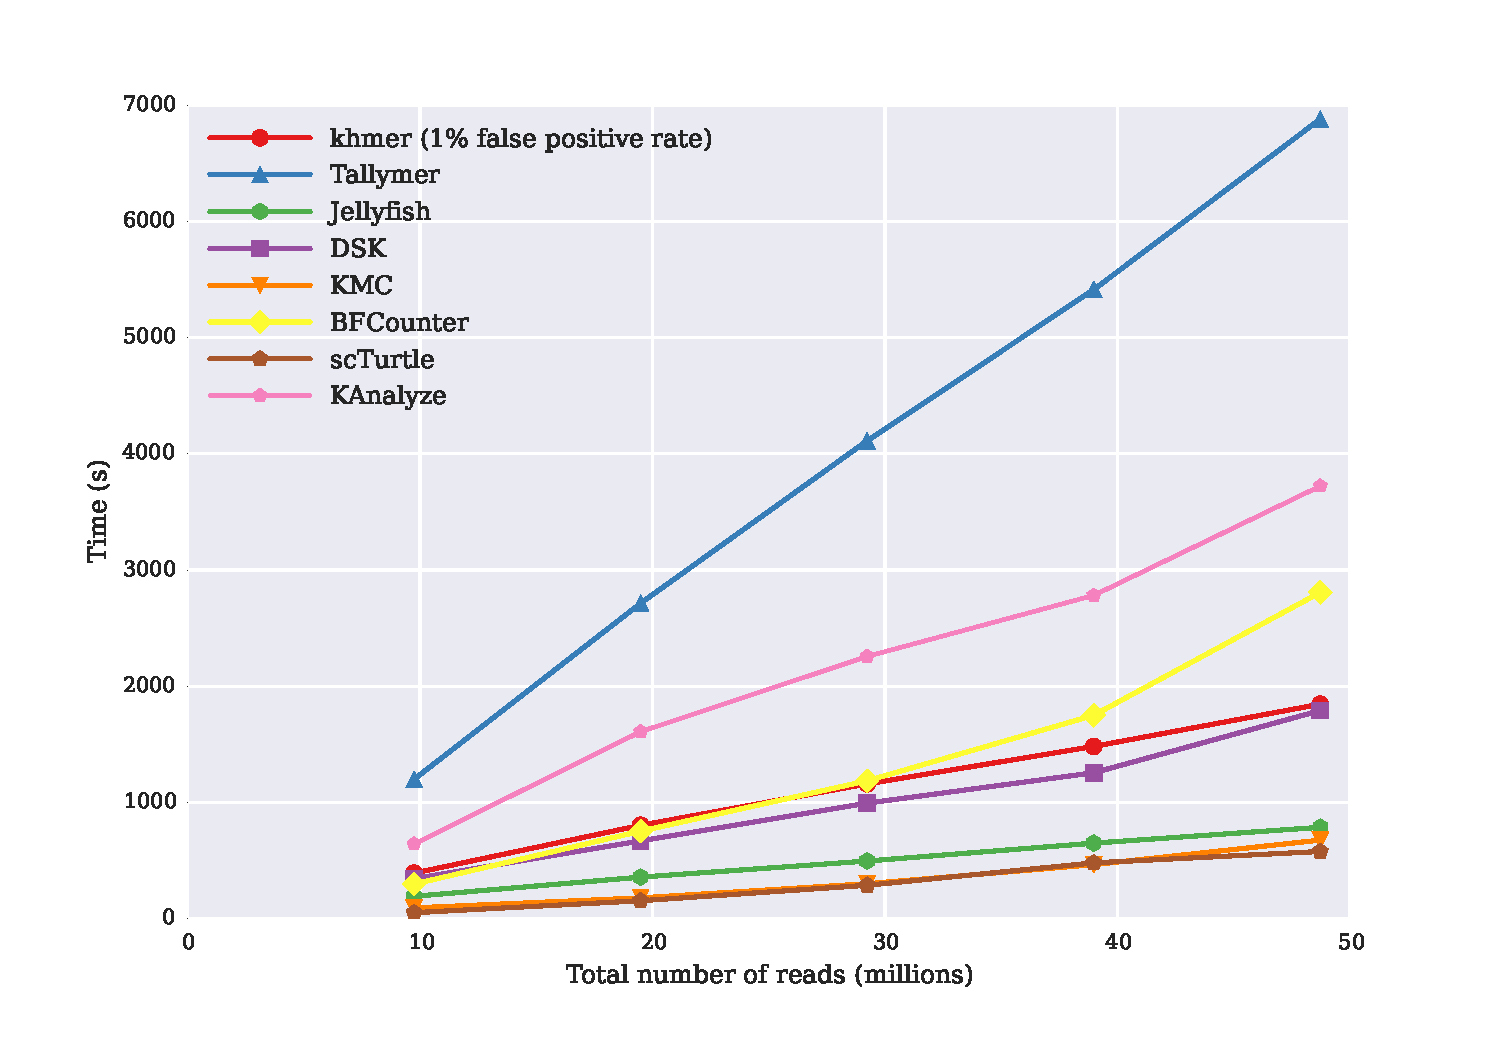
\includegraphics[width=5in]{./figures/figure1_time_benchmark}}

\caption{\bf Comparison of the time it takes for k-mer counting tools
  to calculate k-mer abundance histograms, with time (y axis, in
  seconds) against data set size (in number of reads, x axis).  
  All programs executed in time approximately linear with
  the number of input reads.}

\label{fig:cmp_time}
\end{figure}

\begin{figure}[!ht]
\centerline{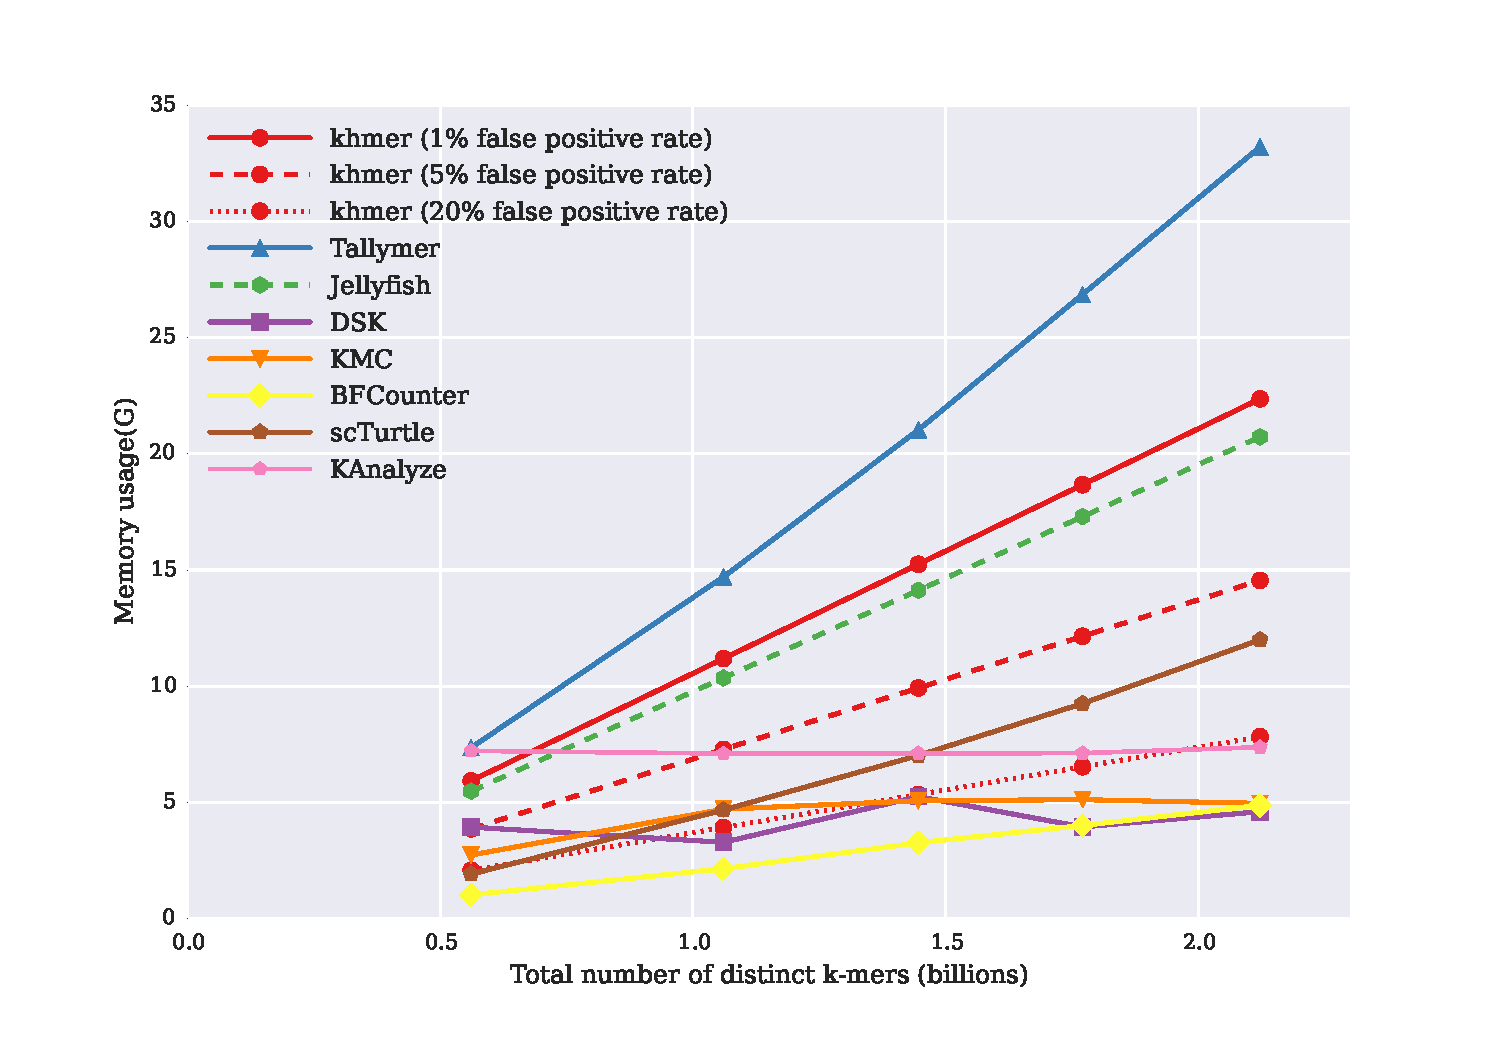
\includegraphics[width=5in]{./figures/figure2_memory_benchmark}}

\caption{\bf Memory usage of k-mer counting tools when calculating
  k-mer abundance histograms, with maximum resident program size (y
  axis, in GB) plotted against the total number of distinct k-mers in
  the data set (x axis, billions of k-mers). }

\label{fig:cmp_memory}
\end{figure}

\begin{figure}[!ht]
\centerline{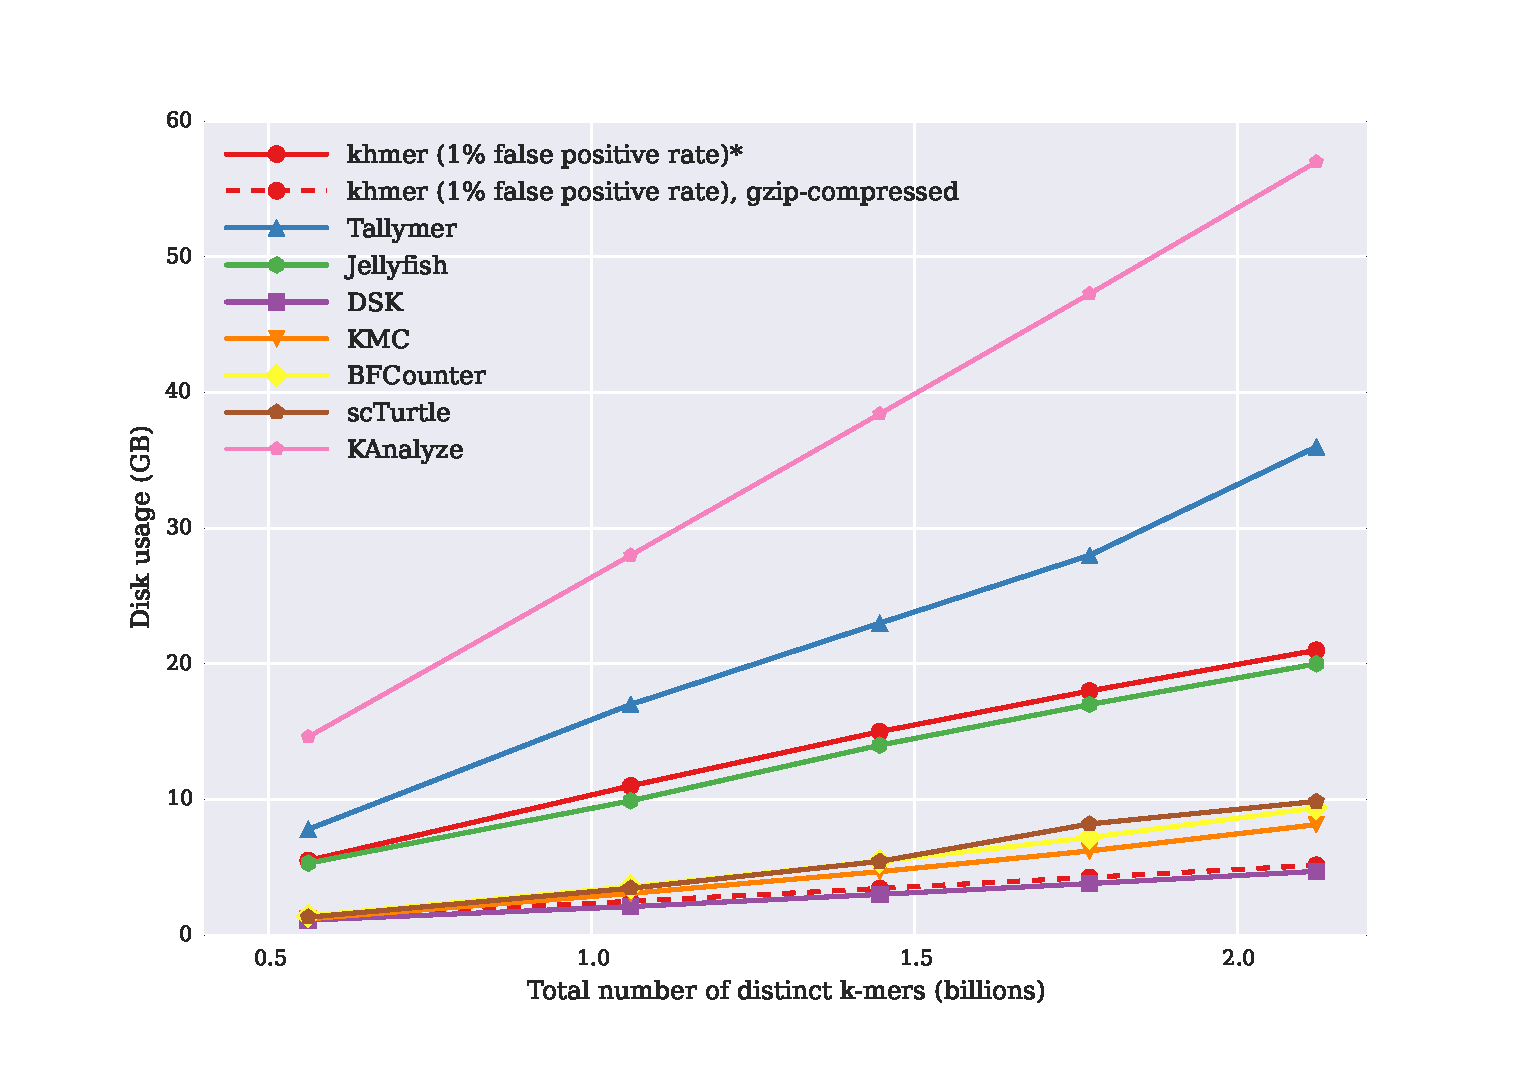
\includegraphics[width=5in]{./figures/figure3_disk_benchmark}}

\caption{\bf Disk storage usage of different k-mer counting tools to
  calculate k-mer abundance histograms in GB (y axis), plotted against
  the number of distinct k-mers in the data set (x axis).  $^*$Note
  that khmer does not use the disk during counting or retrieval,
  although its hash tables can be saved for reuse.}

\label{fig:cmp_disk}
\end{figure}

We measured time and memory required to calculate k-mer abundance
histograms in five soil metagenomic read data sets using khmer,
Tallymer, Jellyfish, DSK, KMC, Turtle, and KAnalyze (Table
\ref{table:datasets}; Figures \ref{fig:cmp_time} and
\ref{fig:cmp_memory}).  We chose to benchmark abundance histograms
because this functionality is common to all the software packages, and
is a common analysis approach for determining assembly parameters
\cite{Chikhi:2014aa}.  We applied each package to increasingly large
subsets of a 50m read soil metagenome data set \cite{Howe2012}. For
the BFCounter, KMC, Turtle and KAnalyze packages, which do not
generate k-mer abundance distribution directly, we output the
frequency of each k-mer to a file but do no further analysis.


khmer offers a general range of useful
performance tradeoffs for disk I/O, time and memory.  From the
performance comparison between khmer and other k-mer counting packages
in calculating k-mer abundance distributions, khmer is comparable with
existing packages. Figure \ref{fig:cmp_time} shows that the time usage of the khmer
approach is comparable to DSK and BFCounter, and, as expected,
increases linearly with data set size. Tallymer is the slowest of the
four tools in this testing, while KMC, Turtle, and Jellyfish are
the fastest. 
From Figure \ref{fig:cmp_memory}, we see that the memory usage of
Jellyfish, Tallymer, BFCounter, and Turtle increases linearly with
data set size. Tallymer uses more memory than Jellyfish generally,
while BFCounter and Turtle have considerably lower memory usage.
DSK, KMC, and KAnalyze use constant memory across the data sets, but
at the cost of more limited functionality (discussed below).

We also measured disk usage during counting.  Figure
\ref{fig:cmp_disk} shows that the disk usage also increases linearly
with the number of k-mers in the data set.  For a high-diversity
metagenomic data set of 5 GB, the disk usage of both Jellyfish and
Tallymer is around 30 GB.  khmer counts k-mers entirely in working
memory and does not rely on any on-disk storage to store or retrieve
k-mer counts, although for practicality the hash tables can be saved
for later reuse; the uncompressed disk usage for khmer in Figure
\ref{fig:cmp_disk} is the same as its memory.  At the expense of more
time, khmer supports saving and loading gzip-compressed hash tables,
which are competitive in size to DSK's on-disk database (Figure 3,
dashed line).


\subsection{khmer memory usage is fixed and low}

The memory usage of the basic Count-Min Sketch approach is fixed:
khmer's memory usage does not increase as data is loaded. While this
means that khmer will never crash due to memory limitations, and all
operations can be performed in main memory without recourse to disk
storage, the false positive rate may grow too high.  Therefore the
memory size must be chosen in light of the false positive rate and
miscount acceptable for a given application.  In practice, we
recommend choosing the maximum available memory, because the false
positive rate decreases with increasing memory and there are no
negative effects to minimizing the false positive rate.

For any given data set, the size and number of hash tables will
determine the accuracy of k-mer counting with khmer.  Thus, the user
can control the memory usage based on the desired level of accuracy
(Figure \ref{fig:cmp_memory}). The time usage for the first step of
k-mer counting, consuming the reads, depends on the total amount of
data, since we must traverse every k-mer in every read.  The second
step, k-mer retrieval, is algorithmically constant for fixed k;
however, for practicality, the hash tables are usually saved to and
loaded from disk, meaning that k-mer retrieval time depends directly
on the size of the database being queried.

The memory usage of khmer is particularly low for sparse data sets,
especially since only main memory is used and no disk space is
necessary beyond that required for the read data sets.  This is no
surprise: the information theoretic comparison in \cite{Pell2012}
shows that, for sparse sequencing data sets, Bloom filters require
considerably less memory than any possible exact information storage
for a wide range of false positive rates and data set sparseness.

In our implementation we use 1 byte to store the count of each k-mer
in the data structure. Thus the maximum count for a k-mer will be 255.
In cases where tracking bigger counts is required, khmer also provides
an option to use an STL map data structure to store counts above 255,
with the trade-off of significantly higher memory usage.  In the
future, we may extend khmer to counters of arbitrary bit sizes.


% Tallymer is not shown in figure, may need modification here - @QP

The memory usage of khmer also increases linearly with data set size
as long as we hold the false positive rate constant.  However, the
memory usage of khmer varies substantially with the desired false
positive rate: we can decrease the memory usage by increasing the
false positive rate as shown in Figure \ref{fig:cmp_memory}.  We also
see that with a low false positive of 1\%, the memory usage is
competitive with Tallymer and Jellyfish; with a higher 5\% false
positive rate, the memory usage is lower than all but the disk-based
DSK; with an false positive rate as high as 20\%, the memory usage is
further lower, close to DSK, KAnalyze, and KMC.


\subsection{khmer accesses k-mer counts efficiently}

% @CTB update for discussion of turtle, KAnalyze, etc.
We measured the time it took to access 9.7m 22-mers across five
different data sets after the initial databases had been built (Figure
\ref{fig:cmp_count}).  Note that Tallymer, Jellyfish, and khmer all
support random access to k-mer counts, while BFCounter, DSK, KMC, Turtle and 
KAnalyze do not. Here, khmer
performed well, dramatically outperforming Jellyfish and Tallymer.  In
all three cases, system time dominated the overall time required to
retrieve k-mers, suggesting that the primary reason for the increase
in retrieval time was due to the increased size of the database on the
disk (data not shown).  In particular, khmer is independent of the
size of the database in retrieval time once the hash tables are loaded
into memory. 


\begin{figure}[!ht]
\centerline{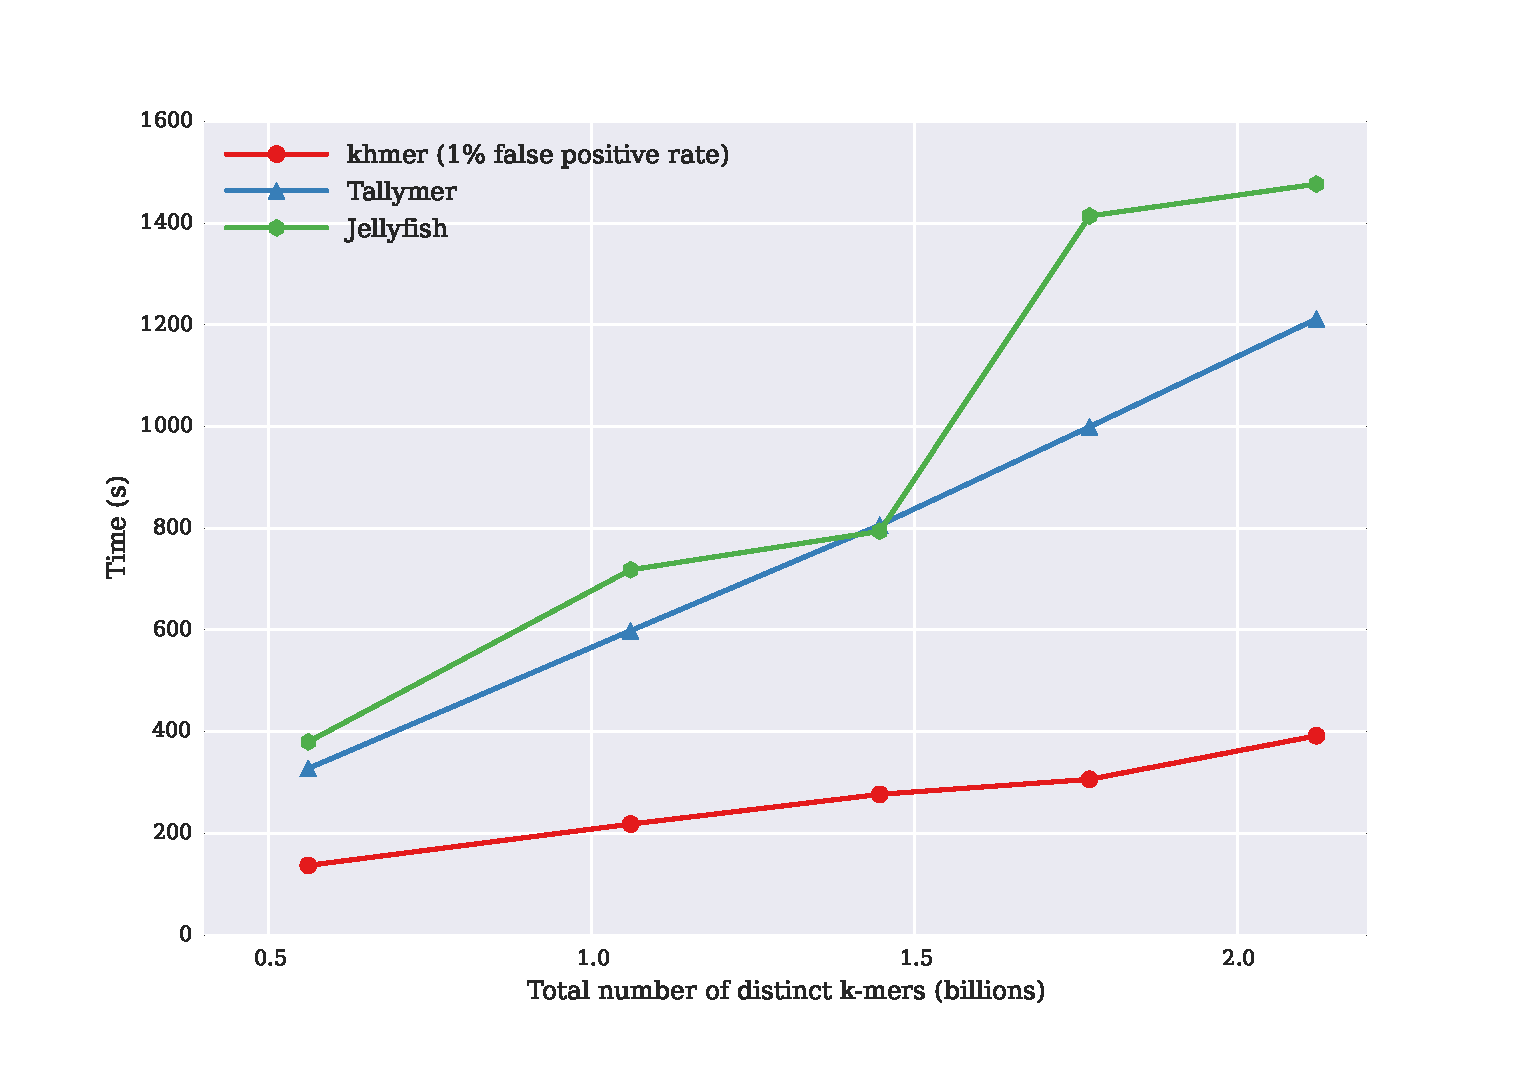
\includegraphics[width=5in]{./figures/figure4_count_benchmark}}
\caption{\bf Time for several k-mer counting tools to retrieve the
  counts of 9.7m randomly chosen k-mers (y axis), plotted against the
  number of distinct k-mers in the data set being queried (x axis).
  BFCounter, DSK, Turtle, KAnalyze, and KMC do not support this functionality.}
\label{fig:cmp_count}
\end{figure}


This highly  memory- and time-efficient online counting is particularly 
important for the streaming approaches to data
analysis needed as data set sizes increase, like digital normalization which 
will be discussed in next chapter and the IGS based method to analyze 
microbial diversity which will be discussed in later chapters.  Because query and
updating of k-mer counts can be done directly as data is being loaded,
with no need for disk access or an indexing step, khmer can also
perform well in situations with poor disk I/O performance.  (Note that
BFCounter also supports online k-mer counting \cite{Melsted2011}.)



\section{False positive rates in k-mer counting are low and predictable}

The Count-Min Sketch is a probabilistic data structure with a one-sided
error that results in random overestimates of k-mer frequency, but
does not generate underestimates. Next we will discuss the characteristics of 
such counting inaccuracy and the influence of such inaccuracy to the real-world 
applications of khmer for k-mer counting.

\subsection{The measured counting error is low on short-read data}


Due to the use of Count-Min Sketch and its lack of collision tracking,
khmer will report some incorrect counts for k-mers; these counts are
always higher than the true counts, up to the bound of 255 (a limit
imposed by our use of 8-bit counters).

In the Count-Min Sketch, the total memory usage is fixed; the memory
usage, the hash functions, and the total number of distinct objects
counted all influence the accuracy of the count.  While the
probability of an inaccurate count can easily be estimated based on
the hash table load, the miscount size is dependent on details of the
frequency distribution of k-mers \cite{Cormode2005}.

More specifically, in the analysis of the Count-Min Sketch, the
difference between the incorrect count and actual count is related to
the total number of k-mers in a data set and the size of each hash
table \cite{Cormode2005}. Further study has shown that the behavior of
Count-Min Sketch depends on specific characteristics of the data set
under consideration, like the distribution of k-mer abundances \cite{Rusu2008,
  CormodeM05}. In general, the average miscount will be small if the data is
left-skewed.  As noted by Melsted and Pritchard, a large number of
k-mers in short-read data are low-abundance, leading to precisely the
skew that would yield low miscounts \cite{Melsted2011}.  Here we use
both real and simulated data sets (Table \ref{table:random_data}) to evaluate the counting performance
in practice.

\begin{table}[!ht]
\caption{
\bf{Data sets used for analyzing miscounts.}}
\begin{tabular}{ | p{5cm} | c | c | c |}
\hline
Data set & Size of data set file & Number of total k-mers & Number of distinct k-mers \\
\hline
Real metagenomics reads                                  & 7.01M  & 2,917,200  & 1,944,996 \\
\hline
Totally random reads with randomly generated k-mers      & 3.53M  & 2,250,006  & 1,973,059 \\
\hline
Simulated reads from simulated genome with error         & 5.92M  & 3,757,479  & 2,133,592 \\
\hline
Simulated reads from simulated genome without error      & 9.07M  & 5,714,973  & 1,989,644 \\
\hline
Real {\em E. coli} reads                                        & 4.85M  & 4,004,911  & 2,079,302 \\
\end{tabular}
\begin{flushleft}
\end{flushleft}
\label{table:random_data}
\end{table}



\begin{figure}[!ht]
\centerline{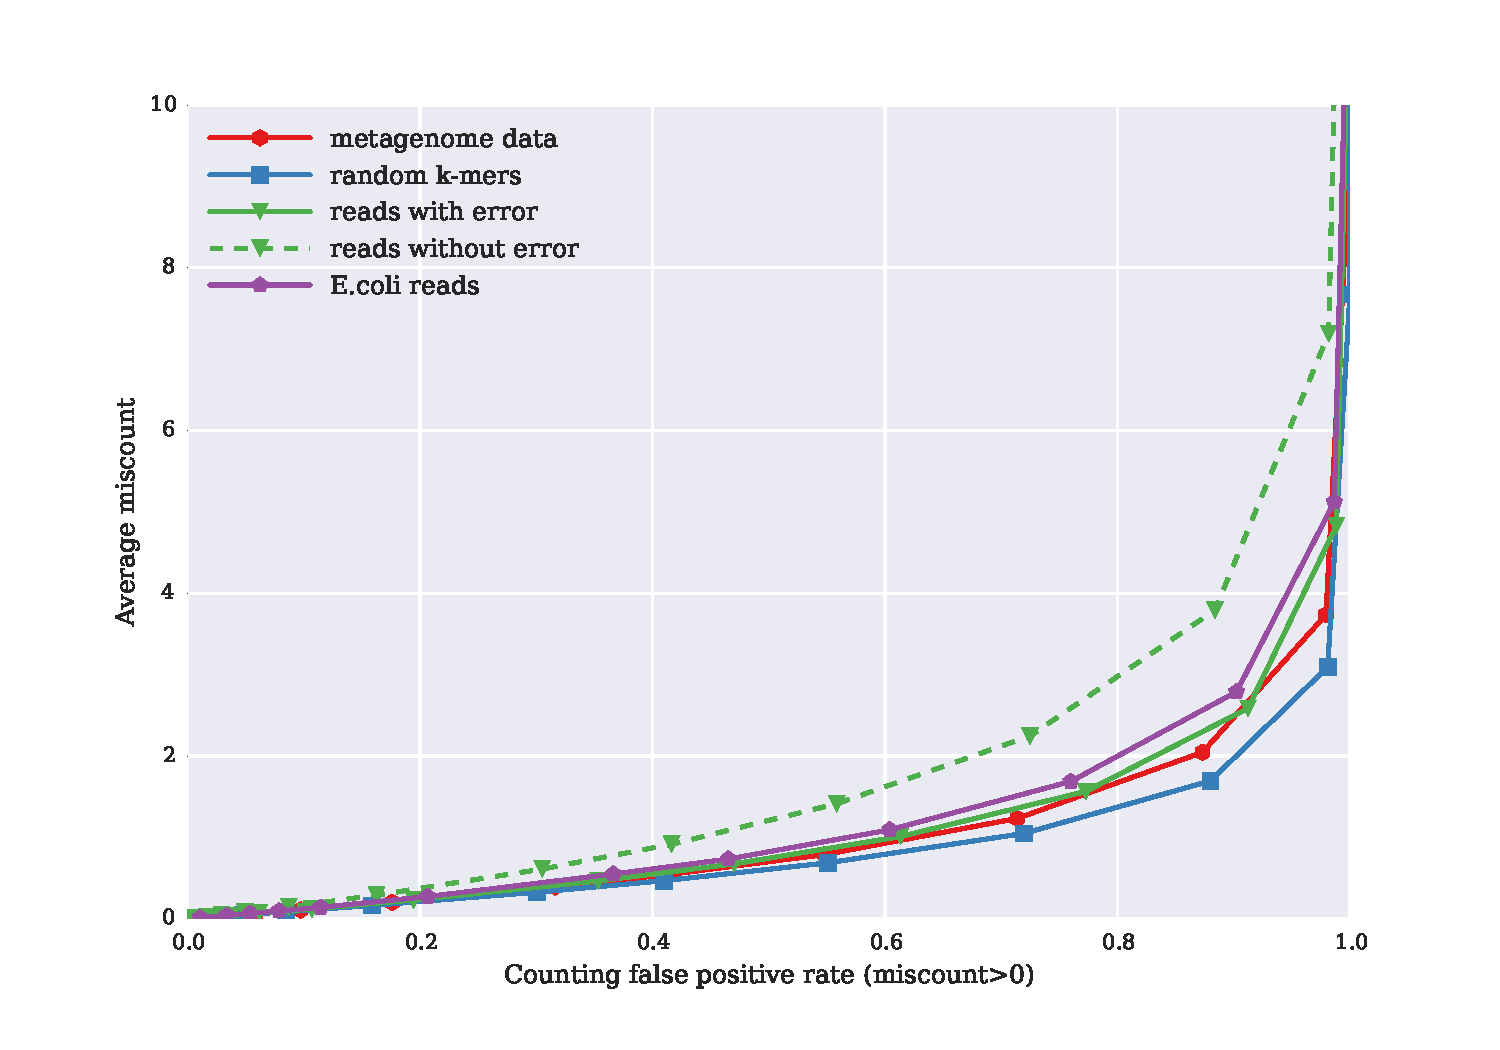
\includegraphics[width=5in]{./figures/figure5_average_offset_vs_fpr}}
\caption{\bf Relation between average miscount --- amount by which
the count for k-mers is incorrect --- on the y axis, plotted against
false positive rate (x axis), for five data sets.  The five data
sets were chosen to have the same total number of distinct k-mers: one
metagenome data set; a set of randomly generated k-mers; a set
of reads, chosen with 3x coverage and 1\% error, from a randomly generated
genome; a simulated set of error-free reads (3x) chosen from a randomly
generated genome and a set of {\em E. coli} reads.}
\label{fig:average_offset_vs_fpr}
\end{figure}

\begin{figure}[!ht]
\centerline{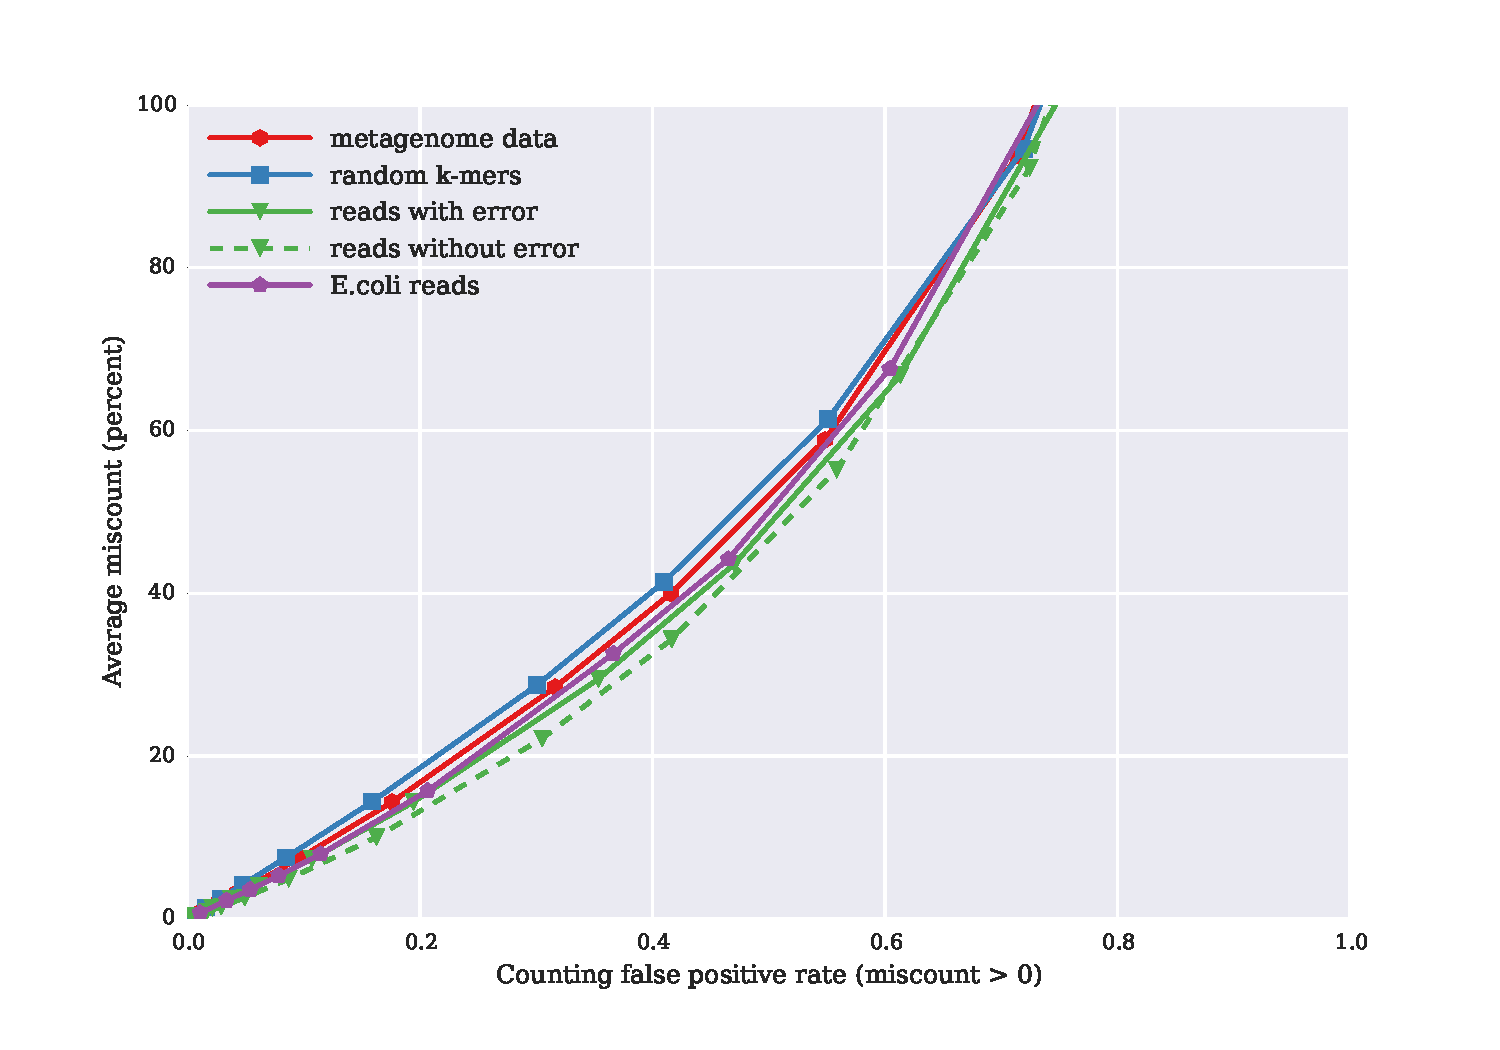
\includegraphics[width=5in]{./figures/figure6_percent_offset_vs_fpr}}
\caption{\bf Relation between percent miscount --- amount by which the
  count for k-mers is incorrect relative to its true count --- on the
  y axis, plotted against false positive rate (x axis), for five data
  sets.  The five data sets are the same as in Figure
  \ref{fig:average_offset_vs_fpr}.}
\label{fig:percent_offset_vs_fpr}
\end{figure}


Figure \ref{fig:average_offset_vs_fpr} shows the relationship between
average miscount and counting false positive rate for five different test data
sets with similar numbers of distinct k-mers: one metagenome data set;
a simulated set of random k-mers; a simulated set of reads, chosen
with 3x coverage and 1\% error; a simulated set of reads (3x) with no
error; and a set of {\em E. coli} reads (Table
\ref{table:random_data}).  Even when the counting false positive rate is as
high as 0.9 --- where 90\% of k-mers have an incorrect count --- the
average miscount is still below 4.

We separately analyzed the average {\em percentage} miscount between
true and false k-mers; e.g. an miscount of 4 for a k-mer whose true
count is 1 would be 400\%.  Figure \ref{fig:percent_offset_vs_fpr}
shows the relationship between average miscount and counting false
positive rate for the same five data sets as in Figure
\ref{fig:average_offset_vs_fpr}.  For a false positive rate of 0.1 (10\% of
k-mer counts are incorrect), the average percentage miscount is less
than 10\% for all five data sets; this will of course generally be
true, because the average miscount is bounded by the product of the
false positive rate with k-mer abundance.

We see here that for a fixed false positive rate, the simulated reads
without error have the highest average miscount, and the randomly
generated k-mers have the lowest average miscount.  This is because
these two abundance distributions have the least and most left-skew,
respectively: the simulated reads without error have no abundance-1
k-mers, while the randomly generated k-mers are entirely low
abundance. Thus, this counting approach is especially suitable for
high diversity data sets, such as metagenomic data, in which a larger
proportion of k-mers are low abundance or unique due to sequencing
errors.


For many applications, an approximate k-mer count is sufficient.  For
example, when eliminating reads with low abundance k-mers, we can
tolerate a certain number of low-frequency k-mers remaining in the
resulting data set falsely.  If RAM-limited we can do the filtering
iteratively so that at each step we are making more effective use of
the available memory.

In practice, we have found that a false positive rate of between 1\%
and 10\% offers acceptable miscount performance for a wide range of
tasks, including error profiling, digital normalization and
low-abundance read-trimming.  Somewhat surprisingly, false positive rates of up
to 80\% can still be used for both read trimming and digital
normalization in memory-limited circumstances, although multiple
passes across the data may be needed.

For many applications, the fact that khmer does not break an imposed
memory bound is extremely useful, since for many data sets ---
especially metagenomic data sets --- high memory demands constrain
analysis \cite{Howe2012,Luo2009}.  Moreover, because the false
positive rate is straightforward to measure, the user can be warned
that the results should be invalidated when too little memory is used.
When combined with the graceful degradation of performance for both
error trimming and digital normalization, khmer readily enables
analysis of extremely large and diverse data sets \cite{adina2013}. In
an experiment to assemble the reads of a soil metagenomic sample
collected from Iowa prairie, the number of reads to assemble drops
from 3.3 million to 2.2 million and the size of the data set drops from
245GB to 145GB accordingly after digital normalization
\cite{Howe2012}.  240GB memory was used in the process. This also
shows that khmer works well to analyze large, real-world metagenomic data
sets.


\subsection{Real-world applications for khmer}

Khmer has been widely used by many research groups for solving different 
bioinformatics problems. It is the foundation of all the work that
will be discussed in this thesis later. We will show the real-worl 
applications of khmer extensively in the chapters next. 

For many applications, an approximate k-mer count is sufficient.  For
example, when eliminating reads with low abundance k-mers, we can
tolerate a certain number of low-frequency k-mers remaining in the
resulting data set falsely.  If RAM-limited we can do the filtering
iteratively so that at each step we are making more effective use of
the available memory.

In practice, we have found that a false positive rate of between 1\%
and 10\% offers acceptable miscount performance for a wide range of
tasks, including error profiling, digital normalization and
low-abundance read-trimming.  Somewhat surprisingly, false positive rates of up
to 80\% can still be used for both read trimming and digital
normalization in memory-limited circumstances, although multiple
passes across the data may be needed.

For many applications, the fact that khmer does not break an imposed
memory bound is extremely useful, since for many data sets ---
especially metagenomic data sets --- high memory demands constrain
analysis \cite{Howe2012,Luo2009}.  Moreover, because the false
positive rate is straightforward to measure, the user can be warned
that the results should be invalidated when too little memory is used.
When combined with the graceful degradation of performance for both
error trimming and digital normalization, khmer readily enables
analysis of extremely large and diverse data sets \cite{adina2013}. In
an experiment to assemble the reads of a soil metagenomic sample
collected from Iowa prairie, the number of reads to assemble drops
from 3.3 million to 2.2 million and the size of the data set drops from
245GB to 145GB accordingly after digital normalization
\cite{Howe2012}.  240GB memory was used in the process. This also
shows that khmer works well to analyze large, real-world metagenomic data
sets.


% E.coli reads dataset has lower "coverage" than simulated reads without error.



\section{Conclusion}

K-mer counting is widely used in bioinformatics, and as sequencing
data set sizes increase, graceful degradation of data structures in
the face of large amounts of data has become important.  This is
especially true when the theoretical and practical effects of the
degradation can be predicted (see e.g. \cite{Melsted2011, Pell2012,
  Roy2014}).  This is a key property of the Count-Min Sketch approach,
and its implementation in khmer.

The khmer software implementation offers good performance, a robust
and well-tested Python API, and a number of useful and well-documented
scripts.  While Jellyfish, DSK, KMC, and Turtle also offer good
performance, khmer is competitive, and, because it provides a Python
API for online counting, is flexible.  In memory-limited situations
with poor I/O performance, khmer is particularly useful, because it
will not break an imposed memory bound and does not require disk
access to store or retrieve k-mer counts.  However, in exchange for
this memory guarantee, counting becomes increasingly incorrect as less
memory is used or as the data set size grows large; in many situations
this may be an acceptable tradeoff.

\section{Data}

\subsection{Code and data set availability}

% @CTB update

The khmer software \cite{khmer} is implemented in C++ in a Python
wrapper, enabling flexible use and reuse by users with a wide range of
computational expertise.  The software package is freely available for
academic and commercial use and redistribution under the BSD license
at github.com/ged-lab/khmer/.  khmer comes with substantial
documentation and many tutorials, and contains extensive unit tests.
Moreover, we have built several applications on top of khmer,
including memory-efficient de Bruijn graph partitioning
\cite{Pell2012} and lossy compression of short-read data sets for
assembly \cite{Brown2012}.

The version of khmer used to generate the results in this chapter is available
at \\
http://github.com/ged-lab/khmer.git, tag '2013-khmer-counting'.
Scripts specific to this paper are available in the paper repository
at \\
https://github.com/ged-lab/2013-khmer-counting.
The IPython\cite{4160251} notebook file and data analysis to generate the figures are also
available in that github repository.  Complete instructions to reproduce
all of the results in this paper are available in the khmer-counting
repository; see README.rst.

\subsection{Sequence Data}

One human gut metagenome reads data set (MH0001) from the 
MetaHIT (Metagenomics of the Human Intestinal Tract) project \cite{Qin2010} was used. 
It contains approximately 59 million reads, each 44bp long; it was trimmed to remove 
low quality sequences. 

Five soil metagenomics reads data sets with different size were taken
from the GPGC project for benchmark purpose (see Table
\ref{table:datasets}).  These reads are from soil in Iowa region and they
are filtered to make sure there are less than 30\% Ns in the read and
each read is longer than 30 bp.  The exact data sets used for the
paper are available on Amazon S3 and the instructions to acquire these
data sets are available in the paper repository on github.com.

We also generated four short-read data sets to assess the false
positive rate and miscount distribution. One is a subset of a real
metagenomics data set from the MH0001 data set, above. The second
consists of randomly generated reads. The third and fourth contain
reads simulated from a random, 1 Mbp long genome.  The third has a
substitution error rate of 3\%, and the fourth contains no errors. The
four data sets were chosen to contain identical numbers of distinct
22-mers.  The scripts necessary to regenerate these data are available
in the paper repository on github.com.




\chapter{A framework for streaming analysis of short DNA sequencing reads based
on k-mer counting}

\section{Introduction}

In last chapter, we introduced an efficient k-mer counting approach based on a
probabilistic data structure. In this chapter, we will discuss the application
of this approach to enable streaming analysis of short DNA sequencing reads.
First, we will show a novel approach to use median k-mer count in a read to estimate
sequencing depth without a reference assembly. Next based on this approach two
streaming methods that are critically important in next generation sequencing
data analysis will be discussed. One is the single-pass method to eliminate redundant reads in
data sets to reduce computational cost in down-streaming analysis like
assembly, which is termed as "digital normalization". The other one is the
method to analyze and trim sequencing errors in short reads dat asets, in a
semi-streaming or streaming fashion.

The approach to use median k-mer count to estimate sequencing depth of a read is
also the foundation of the IGS based diversity analysis approach we will
discuss in the next chapter. The streaming methods to remove redundant reads
and sequencing error analysis and trimming are not directly related to the IGS
based diversity analysis method, nevertheless the applications of the two
streaming methods to facilitate the assembly of metagenomic reads and remove
sequencing errors in reads data sets benefit many bioinformatics approaches,
including the microbial diversity analysis.
% 
% % % 
\section{Estimating sequencing depth without a reference assembly}

Short-read assembly requires deep sequencing to systematically sample the
source genome, because shotgun sequencing is subject to both random sampling
variation and systematic sequencing biases.  For example, 100x sampling of a
human genome is required for recovery of 90\% or more of the genome in contigs
$>$ 1kb \cite{pubmed21187386}. In principle much of this high-coverage data is
redundant and could be eliminated without consequence to the final assembly,
but determining which reads to eliminate requires a per-read estimate of
coverage. Traditional approaches estimate coverage by mapping reads to an
assembly.  This presents a chicken-and-egg problem: to determine which regions
are oversampled, we must already have an assembly!

\begin{figure}[!ht]
\centerline{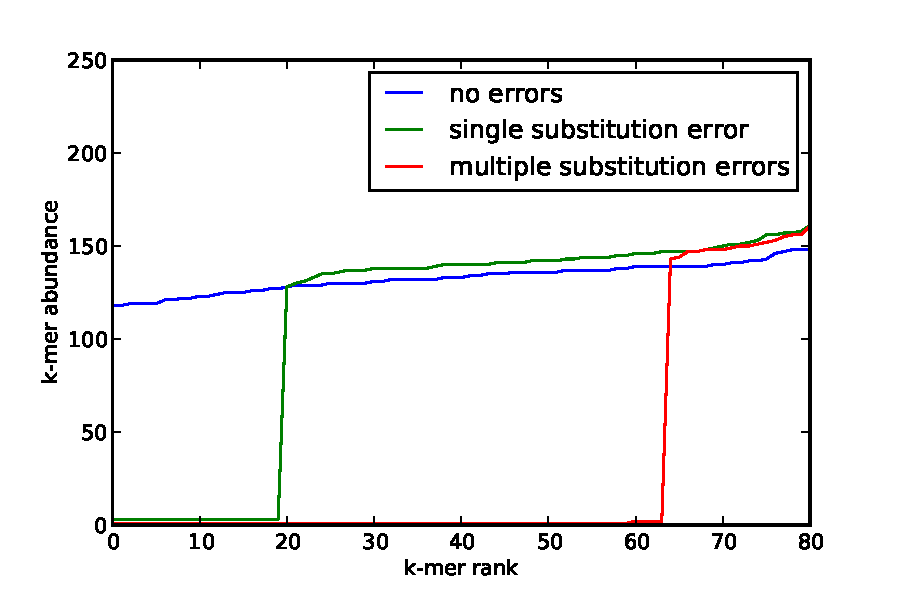
\includegraphics[width=4in]{diginorm-ranks.pdf}} \caption{ {\bf
Representative rank-abundance distributions for 20-mers from 100-base reads
with no errors, a read with a single substitution error, and a read with
multiple substitution errors.}} \label{fig:rankabund} \end{figure}

We may calculate a {\em reference-free} estimate of genome coverage by looking
at the k-mer abundance distribution within individual reads. First, observe
that k-mers, DNA words of a fixed length $k$, tend to have similar abundances
within a read: this is a well-known property of k-mers that stems from each
read originating from a single source molecule of DNA.  The more times a region
is sequenced, the higher the abundance of k-mers from that region would be.  In
the absence of errors, average k-mer abundance could be used as an estimate of
the depth of coverage for a particular read (Figure \ref{fig:rankabund}, ``no
errors'' line).  However, when reads contain random substitution or indel
errors from sequencing, the k-mers overlapping these errors will be of lower
abundance; this feature is often used in k-mer based error correction
approaches \cite{pubmed21114842}.  For example, a single substitution will
introduce $k$ low-abundance k-mers within a read.  (Figure \ref{fig:rankabund},
``single substitution error'' line).  However, for small $k$ and reads of
length $L$ where $L > 3k-1$, a single substitution error will not skew the {\em
median} k-mer abundance.  Only when multiple substitution errors are found in a
single read will the median k-mer abundance be affected (Figure
\ref{fig:rankabund}, ``multiple substitution errors''). The effect of multiple
errors to median k-mer abundance will be discussed in details in next chapter.


\begin{figure}[!ht] \begin{center}
\centerline{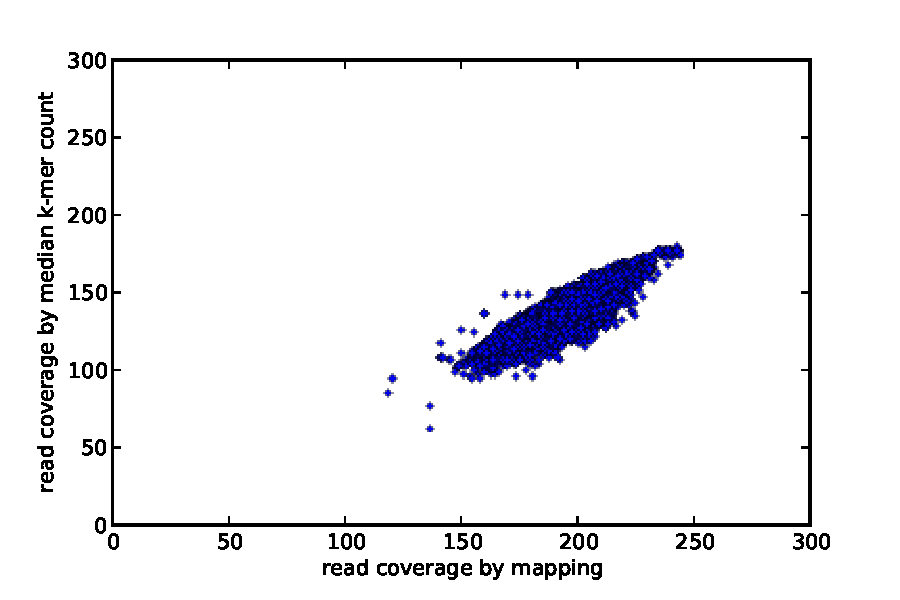
\includegraphics[width=3in]{diginorm-sim-genome.pdf}}
\centerline{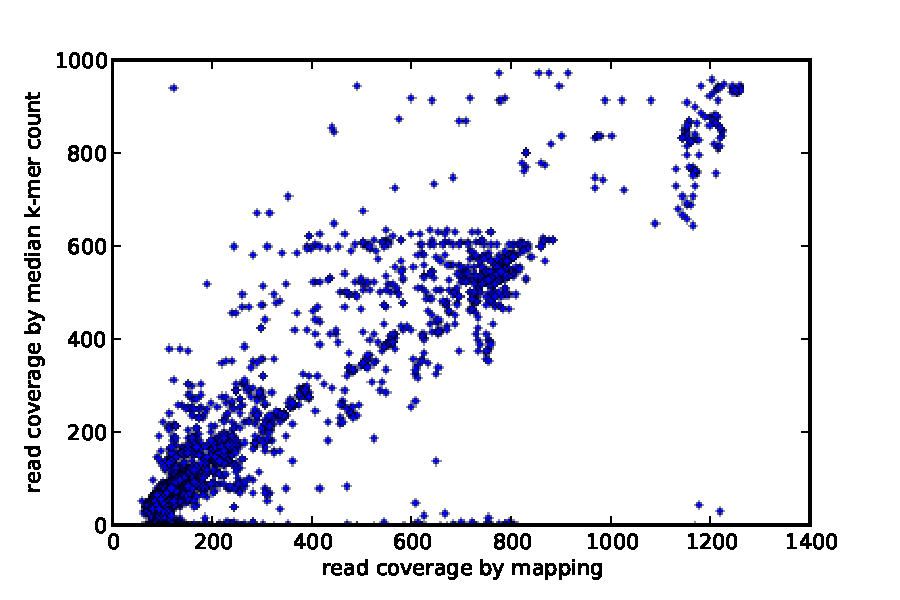
\includegraphics[width=3in]{diginorm-ecoli-genome.pdf}}
\end{center} \caption{ {\bf Mapping and k-mer coverage measures correlate for
simulated genome data and a real {\em E. coli} data set (5m reads).  Simulated
data $r^2 = 0.79$; {\em E. coli} $r^2 = 0.80$.}
}
\label{fig:random} \end{figure}


\begin{figure}[!ht] \begin{center}
\centerline{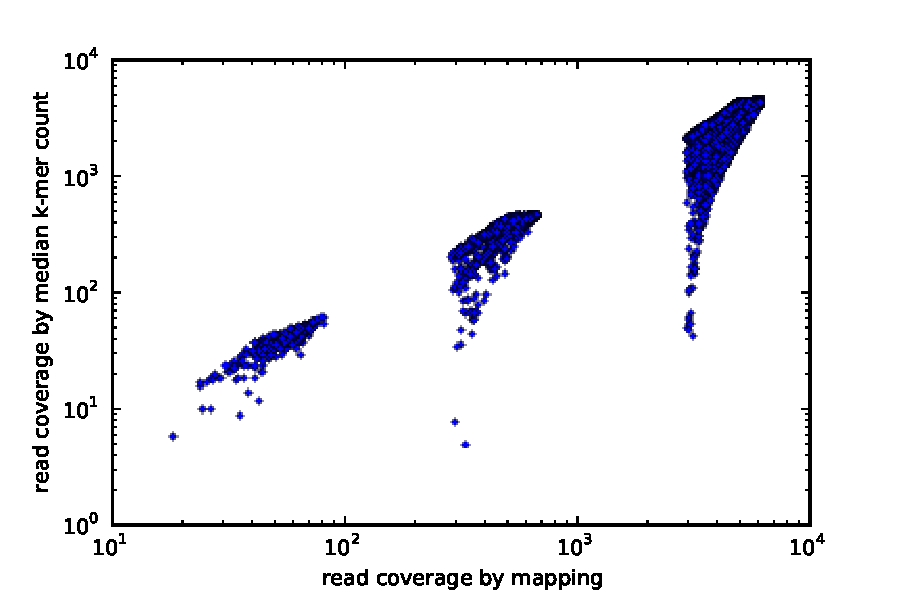
\includegraphics[width=3in]{diginorm-sim-transcr.pdf}}
\centerline{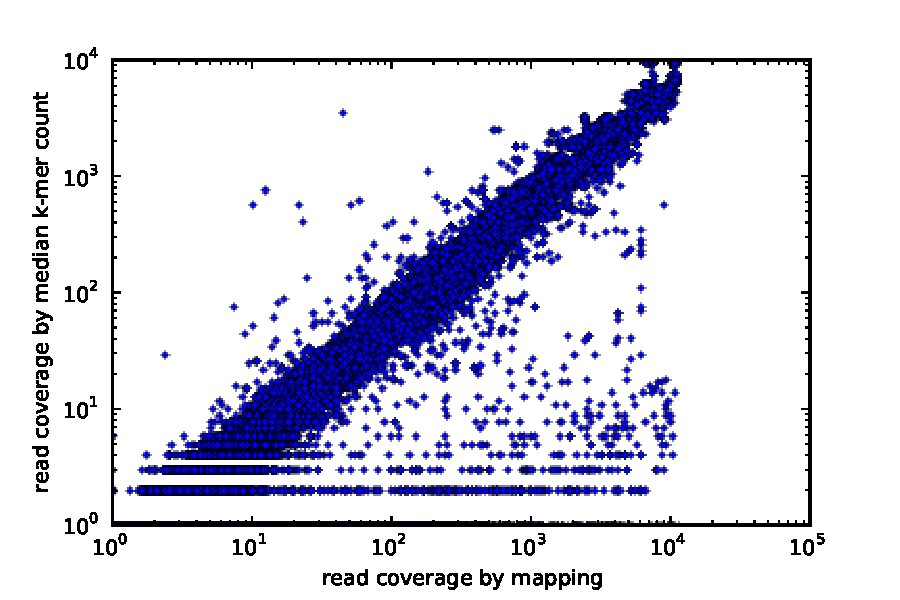
\includegraphics[width=3in]{diginorm-mouse-transcr.pdf}}
\end{center} \caption{ {\bf Mapping and k-mer coverage measures correlate for
simulated transcriptome data as well as real mouse transcriptome data.
Simulated data $r^2 = 0.93$; mouse transcriptome $r^2 = 0.90$.}
}
\label{fig:transcripts} \end{figure}


Using a fixed-memory CountMin Sketch data structure to count k-mers (see
Methods and \cite{countminsketch}), we find that median k-mer abundance
correlates well with mapping-based coverage for artificial and real genomic
data sets.  There is a strong correlation between median k-mer abundance and
mapping-based coverage both for simulated 100-base reads generated with 1\%
error from a 400kb artificial genome sequence ($r^2 = 0.79$; also see Figure
\ref{fig:random}a), as well as for real short-read data from {\em E. coli}
($r^2 = 0.80$, also see Figure \ref{fig:random}b).  This correlation also holds
for simulated and real mRNAseq data: for simulated transcriptome data, $r^2 =
0.93$ (Figure \ref{fig:transcripts}a), while for real mouse transcriptome data,
$r^2 = 0.90$ (Figure \ref{fig:transcripts}b). Thus the median k-mer abundance
of a read correlates well with mapping-based estimates of read coverage.

The coverage on read level estimated from median k-mer count of a read is
always smaller than the mapping-based estimates of read coverage, which is
essentially the coverage on nucleotide level. There is a way to convert the
coverage on read level into real sequencing depth(coverage on nucleotide
level). To cover a k-mer by a read, all the nucleotide in this k-mer must be
covered by the read. If the coverage in nucleotide level is C\_N, the coverage
of a k-mer in a genome will be C\_N * (L-k+1)/L, with length of reads as L.
\cite{Kelley2010} Figure \ref{fig:random} and Figure \ref{fig:transcripts}
shows such relationship obviously.

Such difference between coverage on read level and on nucleotide level is
important in the IGS based diversity analysis method, which will be discussed
in more details in next chapter. For the streaming methods to analyze short
reads data discussed in this chapter, the coverage means the coverage on read
level estimated from median k-mer abundance in a read.



\section{A streaming algorithm to digitally normalize the coverage distribution
of data sets}

Below, we introduce ``digital normalization'', a single-pass lossy compression
algorithm for elimination of redundant reads in data sets based on saturating
coverage of a de Bruijn graph.   While several non-streaming implementations
exist, including Trinity's {\em in silico} normalization
\cite{Haas2013,Brown2012blog}, digital normalization can be efficiently
implemented as a {\em streaming} algorithm.  Critically, no reference sequence
is needed to apply digital normalization.  Digital normalization is inspired by
experimental normalization techniques developed for cDNA library preparation,
in which hybridization kinetics are exploited to reduce the copy number of
abundant transcripts prior to sequencing\cite{pubmed8889548,pubmed7937745}.
{\em Digital} normalization works after sequencing data has been generated,
progressively removing high-coverage reads from shotgun data sets.  This
normalizes average coverage to a specified value, reducing sampling variation
while removing reads, and also removing the many errors contained {\em within}
those reads.  This data and error reduction results in dramatically decreased
computational requirements for {\em de novo} assembly.  This has the advantage
of enabling low-memory preprocessing of both high-coverage genomic data sets,
as well as mRNAseq or metagenomic data sets with high-coverage components
\cite{Brown2012, Howe2012}. Moreover, unlike experimental normalization where
abundance information is removed prior to sequencing, in digital normalization
this information can be recovered from the unnormalized reads.

We present here a fixed-memory implementation of digital normalization that
operates in time linear with the size of the input data.  We then demonstrate
its effectiveness for reducing compute requirements for {\em de novo} assembly
on several real data sets.  These data sets include {\em E. coli} genomic data,
data from two single-cell MD-amplified microbial genomes, and yeast and mouse
mRNAseq.

\subsection{Eliminating redundant reads reduces variation in sequencing depth}

Deeply sequenced genomes contain many highly covered loci.  For example, in a
human genome sequenced to 100x average coverage, we would expect 50\% or more
of the reads to have a coverage greater than 100. In practice, we need many
fewer of these reads to assemble the source locus.

Using the median k-mer abundance estimator discussed above, we can examine each
read in the data set progressively to determine if it is high coverage.  At the
beginning of a shotgun data set, we would expect many reads to be entirely
novel and have a low estimated coverage.  As we proceed through the data set,
however, average coverage will increase and many reads will be from loci that
we have already sampled sufficiently.

Suppose we choose a coverage threshold $C$ past which we no longer wish to
collect reads. If we only keep reads whose estimated coverage is less than $C$,
and discard the rest, we will reduce the average coverage of the data set to
$C$.  This procedure is algorithmically straightforward to execute: we examine
each read's estimated coverage, and retain only those whose coverage is less
than $C$. The following pseudocode provides one approach: 
\begin{verbatim}
   for read in dataset:
      if estimated_coverage(read) < C:
         accept(read)
      else:
         discard(read)
\end{verbatim}
\noindent
\noindent 
where accepted reads contribute to the
$\tt estimated\_coverage$ function.  Note that for any data set with an average
coverage $> 2C$, this has the effect of discarding the majority of reads.
Critically, low-coverage reads, especially reads from undersampled regions,
will always be retained.


\begin{figure}[!ht]
\centerline{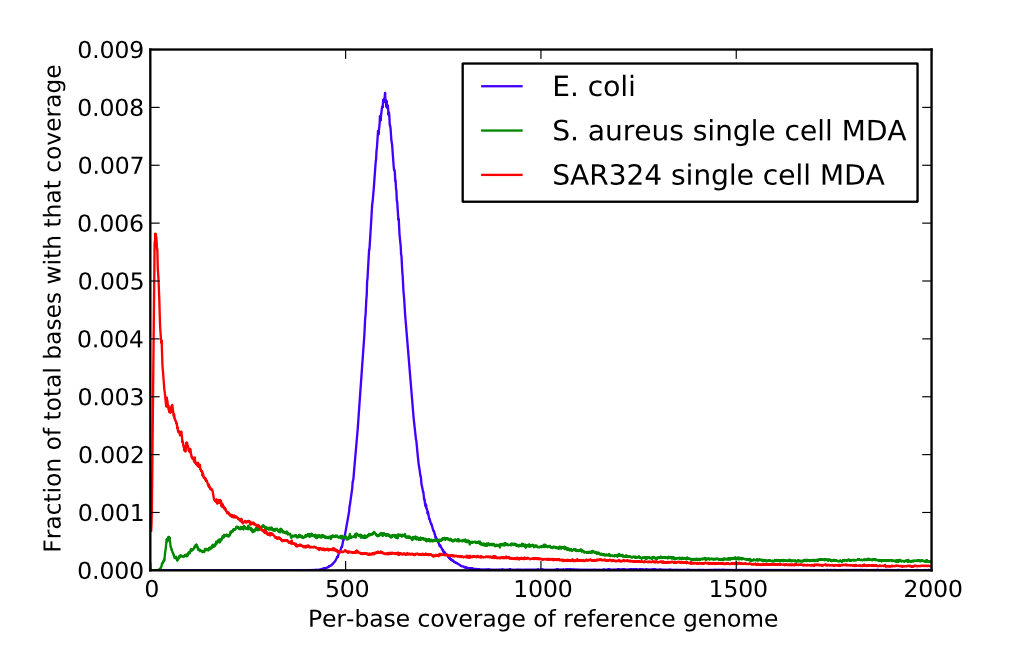
\includegraphics[width=4in]{diginorm-coverage2-raw.png}}
\centerline{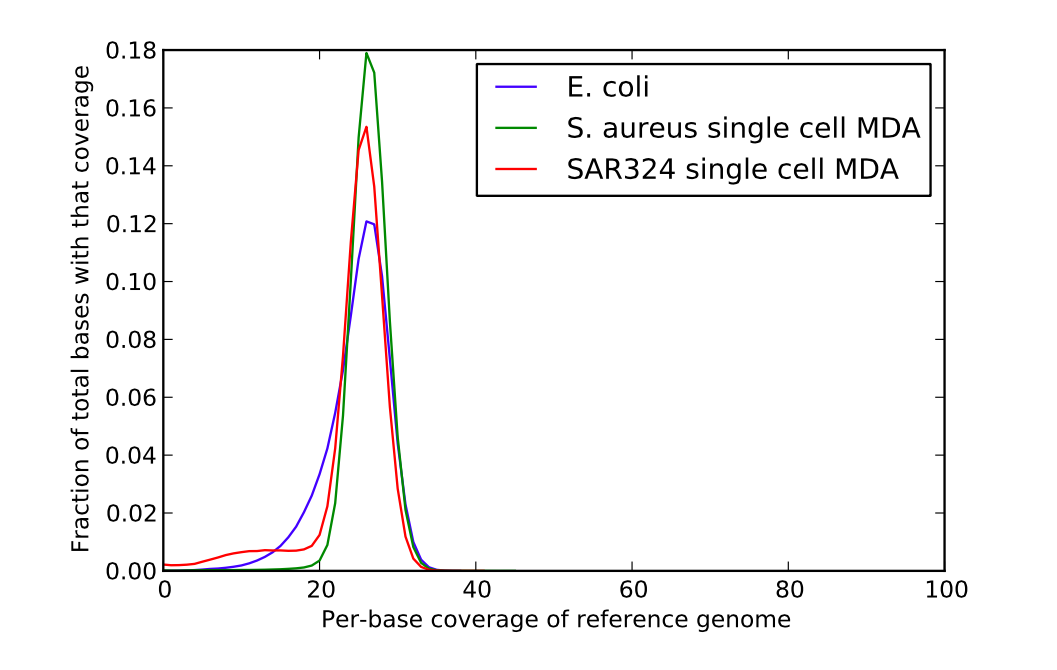
\includegraphics[width=4in]{diginorm-coverage2-dn.png}}
\caption{
{\bf Coverage distribution of three microbial genome samples, calculated
from mapped reads (a) before and (b) after digital normalization (k=20, C=20).}}
\label{fig:coverage}
\end{figure}


The net effect of this procedure, which we call digital normalization, is to
normalize the coverage distribution of data sets.  In Figure
\ref{fig:coverage}a, we display the estimated coverage of an {\em E. coli}
genomic data set, a {\em S. aureus} single-cell MD-amplified data set, and an
MD-amplified data set from an uncultured {\em Deltaproteobacteria}, calculated
by mapping reads to the known or assembled reference genomes (see
\cite{pubmed21926975} for the data source).  The wide variation in coverage for
the two MDA data sets is due to the amplification procedure
\cite{pubmed17487184}.  After normalizing to a k-mer coverage of 20, the high
coverage loci are systematically shifted to an average mapping coverage of 26,
while lower-coverage loci remain at their previous coverage.  This smooths out
coverage of the overall data set.


\begin{figure}[!ht]
\centerline{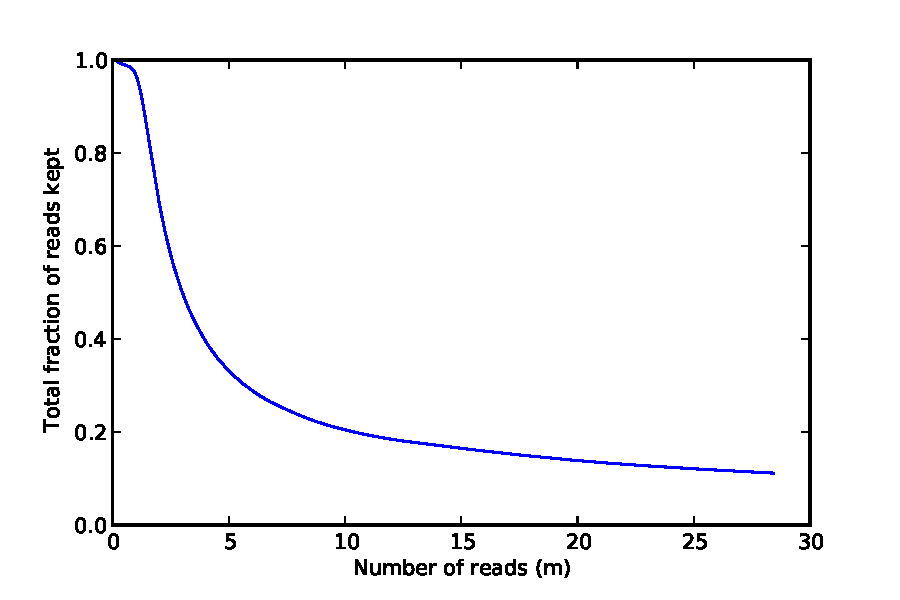
\includegraphics[width=4in]{diginorm-accumulation.pdf}}
\caption{
{\bf Fraction of reads kept when normalizing the {\em E. coli} dataset to C=20 at k=20.}}
\label{fig:accumulate}
\end{figure}


At what rate are sequences retained?  For the {\em E. coli} data set, Figure
\ref{fig:accumulate} shows the fraction of sequences retained by digital
normalization as a function of the total number of reads examined when
normalizing to C=20 at k=20.  There is a clear saturation effect showing that
as more reads are examined, a smaller fraction of reads is retained; by 5m
reads, approximately 50-100x coverage of {\em E. coli}, under 30\% of new reads
are kept.  This demonstrates that as expected, only a small amount of novelty
(in the form of either new information, or the systematic accumulation of
errors) is being observed with increasing sequencing depth.

Here we show that digital normalization provides a general strategy for applying
online or streaming approaches to analysis of {\em de novo} sequencing
data.  The basic algorithm presented here is explicitly a single-pass or streaming
algorithm, in which the entire data set is never considered as a
whole; rather, a partial ``sketch'' of the data set is retained and
used for progressive filtering.  Online algorithms and sketch data
structures offer significant opportunities in situations where data
sets are too large to be conveniently stored, transmitted, or analyzed
\cite{muthukrishnan2005data}.  This can enable increasingly efficient
downstream analyses.
Digital normalization can be applied in any situation where the
abundance of particular sequence elements is either unimportant or can be
recovered more efficiently after other processing, as in assembly, which we will discuss
next.




\subsection{Digital normalization scales assembly of microbial genomes}

We applied the digital normalization and error trimming protocol to
three real data sets from Chitsaz et al (2011) \cite{pubmed21926975}. For all three samples, the number of reads
remaining after digital normalization was reduced by at least 30-fold, while
the memory and time requirements were reduced 10-100x.

%@@(For benchmarking, we used a more recent version of Velvet rather than
%Velvet-SC, because optimizations have been added to Velvet since the Velvet-SC
%fork.)
%
Despite this dramatic reduction in data set size and computational requirements
for assembly, both the {\em E. coli} and {\em S. aureus} assemblies overlapped
with the known reference sequence by more than 98\%.  This confirms that little
or no information was lost during the process of digital normalization;
moreover, it appears that digital normalization does not significantly affect
the assembly results. (Note that we did not perform scaffolding, since the
digital normalization algorithm does not take into account paired-end
sequences, and could mislead scaffolding approaches.  Therefore, these results
cannot directly be compared to those in Chitsaz et al. (2011)
\cite{pubmed21926975}.)

The {\em Deltaproteobacteria} sequence also assembled well, with 98.8\%
sequence overlap with the results from Chitsaz et al. Interestingly, only 30kb
of the sequence assembled with Velvet-SC in Chitsaz et al. (2011) was missing,
while an additional 360kb of sequence was assembled only in the normalized
samples.  Of the 30kb of missing sequence, only 10\% matched via TBLASTX to a
nearby {\em Deltaproteobacteria} assembly, while more than 40\% of the
additional 360kb matched to the same {\em Deltaproteobacteria} sample.
Therefore these additional contigs likely represents real sequence, suggesting
that digital normalization is competitive with Velvet-SC in terms of
sensitivity.

%% @@ better assembly?
%% 
% @ tables or anything?
% 


\begin{table}[!ht]
\caption{
\bf{Single-pass digital normalization to C=20 reduces computational
requirements for transcriptome assembly.}}

%add yeast

\begin{tabular}{|l|c|c|c|c|}

Data set & N reads pre/post & Assembly time pre/post & Assembly memory pre/post \\
 \hline \\
Yeast (Oases) & 100m / 9.3m & 181 min / 12 min (15.1x) & 45.2gb / 8.9gb (5.1x) \\
Yeast (Trinity) & 100m / 9.3m & 887 min / 145 min (6.1x) & 31.8gb / 10.4gb (3.1x) \\
Mouse (Oases) & 100m / 26.4m & 761 min/ 73 min (10.4x) & 116.0gb / 34.6gb (3.4x) \\
Mouse (Trinity) & 100m / 26.4m & 2297 min / 634 min (3.6x) & 42.1gb / 36.4gb (1.2x) \\
\end{tabular}

\begin{flushleft}
\end{flushleft}
\label{tab:dntrans}
\end{table}


\subsection{Digital normalization scales assembly of transcriptomes}


We next applied single-pass digital normalization to published yeast and mouse
mRNAseq data sets, reducing them to 20x coverage at k=20 \cite{pubmed21572440}.
Digital normalization on these samples used 8gb of memory and took about 1 min
per million reads.  We then assembled both the original and normalized sequence
reads with Oases and Trinity, two {\em de novo} transcriptome assemblers (Table
\ref{tab:dntrans}) \cite{pubmed22368243,pubmed21572440}.
%  (Note that
%due to differing execution parameters, the Oases runtimes cannot be directly
%compared to the Trinity runtimes.)
%
For both assemblers the computational resources necessary to complete an
assembly were reduced (Table \ref{tab:dntrans}), but normalization had
different effects on performance for the different samples.  On the yeast data
set, time and memory requirements were reduced significantly, as for Oases
running on mouse.  However, while Trinity's runtime decreased by a factor of
three on the normalized mouse data set, the memory requirements did not
decrease significantly.  This may be because the mouse transcriptome is 5-6
times larger than the yeast transcriptome, and so the mouse mRNAseq is lower
coverage overall; in this case we would expect fewer errors to be removed by
digital normalization.


\begin{table}[!ht]
\caption{
\bf{Digital normalization has assembler-specific effects on transcriptome
assembly.}}

%add yeast

\begin{tabular}{|l|c|c|c|c|}

Data set & Contigs $>$ 300 & Total bp $>$ 300 & Contigs $>$ 1000 & Total bp $>$ 1000 \\
\hline \\
Yeast (Oases) & 12,654 / 9,547 & 33.2mb / 27.7mb & 9,156 / 7,345 & 31.2mb / 26.4mb \\
Yeast (Trinity) & 10,344 / 12,092 & 16.2mb / 16.5mb & 5,765 / 6,053 & 13.6 mb / 13.1mb \\
Mouse (Oases) & 57,066 / 49,356 & 98.1mb / 84.9mb & 31,858 / 27,318 & 83.7mb / 72.4mb \\
Mouse (Trinity) & 50,801 / 61,242 & 79.6 mb / 78.8mb & 23,760 / 24,994 & 65.7mb / 59.4mb \\

\end{tabular}

\begin{flushleft}
\end{flushleft}
\label{tab:dntrans0}
\end{table}


The resulting assemblies differed in summary statistics (Table
\ref{tab:dntrans0}).  For both yeast and mouse, Oases lost 5-10\% of total
transcripts and total bases when assembling the normalized data.  However,
Trinity {\em gained} transcripts when assembling the normalized yeast and mouse
data, gaining about 1\% of total bases on yeast and losing about 1\% of total
bases in mouse.  Using a local-alignment-based overlap analysis (see Methods)
we found little difference in sequence content between the pre- and post-
normalization assemblies: for example, the normalized Oases assembly had a
98.5\% overlap with the unnormalized Oases assembly, while the normalized
Trinity assembly had a 97\% overlap with the unnormalized Trinity assembly.

To further investigate the differences between transcriptome assemblies caused
by digital normalization, we looked at the sensitivity with which long
transcripts were recovered post-normalization.  When comparing the normalized
assembly to the unnormalized assembly in yeast, Trinity lost only 3\% of the
sequence content in transcripts greater than 300 bases, but 10\% of the
sequence content in transcripts greater than 1000 bases.  However, Oases lost
less than 0.7\% of sequence content at 300 and 1000 bases.  In mouse, we see
the same pattern. This suggests that the change in summary statistics for
Trinity is caused by fragmentation of long transcripts into shorter
transcripts, while the difference for Oases is caused by loss of splice
variants.  Indeed, this loss of splice variants should be expected, as there
are many low-prevalence splice variants present in deep sequencing data
\cite{pubmed21151575}. Interestingly, in yeast we recover {\em more}
transcripts after digital normalization; these transcripts appear to be
additional splice variants.

% @table of splice foo?



\begin{table}[!ht]
\caption{
\bf{Digital normalization to C=20 removes many erroneous k-mers from sequencing data sets.  Numbers
in parentheses indicate number of true k-mers lost at each step, based on reference.}}
\begin{tabular}{|l|c|c|c|c|c|}
Data set & True 20-mers & 20-mers in reads & 20-mers at C=20 & \% reads kept\\
\hline \\
Simulated genome & 399,981 & 8,162,813 & 3,052,007 (-2) & 19\% \\
Simulated mRNAseq & 48,100 & 2,466,638 (-88) & 1,087,916 (-9) & 4.1\% \\
{\em E. coli} genome & 4,542,150 & 175,627,381 (-152) & 90,844,428 (-5) & 11\% \\
Yeast mRNAseq & 10,631,882 & 224,847,659 (-683) & 10,625,416 (-6,469) & 9.3\% \\
Mouse mRNAseq & 43,830,642 & 709,662,624 (-23,196) & 43,820,319 (-13,400) & 26.4\% \\
\end{tabular}
\begin{flushleft}
\end{flushleft}
\label{tab:normC20}
\end{table}

\begin{table}[!ht]
\caption{
\bf{Three-pass digital normalization removes most erroneous k-mers.  Numbers
in parentheses indicate number of true k-mers lost at each step, based on known reference.}}
\begin{tabular}{|l|c|c|c|c|}
Data set & True 20-mers & 20-mers in reads & 20-mers remaining & \% reads kept\\
\hline \\
Simulated genome & 399,981 & 8,162,813 & 453,588 (-4) & 5\% \\
Simulated mRNAseq & 48,100 & 2,466,638 (-88) & 182,855 (-351) & 1.2\% \\
{\em E. coli} genome & 4,542,150 & 175,627,381 (-152) & 7,638,175 (-23) & 2.1\% \\
Yeast mRNAseq & 10,631,882 & 224,847,659 (-683) & 10,532,451 (-99,436) & 2.1\% \\
Mouse mRNAseq & 43,830,642 & 709,662,624 (-23,196) & 42,350,127 (-1,488,380) & 7.1\% \\
\end{tabular}
\begin{flushleft}
\end{flushleft}
\label{tab:normC5}
\end{table}

% 
The difference between Oases and Trinity results show that Trinity is more
sensitive to digital normalization than Oases: digital normalization seems to
cause Trinity to fragment long transcripts. Why?  One potential issue is that
Trinity only permits k=26 for assembly, while normalization was performed at
k=20; digital normalization may be removing 26-mers that are important for
Trinity's path finding algorithm.  Alternatively, Trinity may be more sensitive
than Oases to the change in coverage caused by digital normalization.
Regardless, the strong performance of Oases on digitally normalized samples, as
well as the high retention of k-mers (Table \ref{tab:normC20}) suggests that
the primary sequence content for the transcriptome remains present in the
normalized reads, although it is recovered with different effectiveness by the
two assemblers.


\subsection{lower bound on memory usage for effective digital normalization}

In this section, we will discuss the lower bound on memory usage for effective digital
normalization and the effects of high false positive rates particularly.

\begin{table}[!ht]
\caption{ \bf{Low-memory digital normalization. The results of
    digitally normalizing a 5m read {\em E. coli} data set (1.4 GB) to C=20
    with k=20 under several memory usage/false positive rates.  The
    false positive rate (column 1) is empirically determined.  We
    measured reads remaining, number of ``true'' k-mers missing from
    the data at each step, and the number of total k-mers remaining.
    Note: at high false positive rates, reads are erroneously removed due to
    inflation of k-mer counts.}}
\begin{tabular}{ | c | c | c | c | c | c | c |}
\hline
memory   & FP rate & retained reads & retained reads \% & true k-mers missing & total k-mers \\
\hline
before diginorm   &  -      & 5,000,000   & 100.0\%    & 170  &  41.6m \\
2400 MB           &   0.0\% & 1,656,518   &  33.0\%    & 172  &  28.1m \\
240 MB            &   2.8\% & 1,655,988   &  33.0\%    & 172  &  28.1m \\
120 MB            &  18.0\% & 1,652,273   &  33.0\%    & 172  &  28.1m \\
60 MB             &  59.1\% & 1,633,182   &  32.0\%    & 172  &  27.9m \\
40 MB             &  83.2\% & 1,602,437   &  32.0\%    & 172  &  27.6m \\
20 MB             &  98.8\% & 1,460,936   &  29.0\%    & 172  &  25.7m \\
10 MB             & 100.0\% & 1,076,958   &  21.0\%    & 185  &  20.9m \\
\end{tabular}
\begin{flushleft}
\end{flushleft}
\label{table:loop_norm}
\end{table}

\begin{table}[!ht]
\caption{
\bf{{\em E. coli} genome assembly after low-memory digital normalization.
  A comparison of assembling reads digitally normalized with low memory/high
  false positive rates.  The reads were digitally normalized to 
  C=20 (see
  \cite{Brown2012} for more information) and were assembled using Velvet.
  We measured total length of assembly,
  as well as percent of true MG1655 genome covered by the assembly using QUAST.}}
\begin{tabular}{ | c | c | c | c | c | c |}
\hline
memory   & FP rate & N contigs & total length(bases) & \% of true genome covered \\
\hline
before diginorm  &-   & 106 & 4,546,051 & 97.84\% \\
    2400 MB  &  0.0\% & 617 & 4,549,235 & 98.05\% \\
     240 MB  &  2.8\% &  87 & 4,549,253 & 98.04\% \\
     120 MB  & 18.0\% &  86 & 4,549,335 & 98.04\% \\
      60 MB  & 59.1\% &  90 & 4,548,619 & 98.03\% \\
      40 MB  & 83.2\% &  89 & 4,550,599 & 98.11\% \\
      20 MB  & 98.8\% &  85 & 4,550,014 & 98.04\% \\
      10 MB  &100.0\% &  97 & 4,545,871 & 97.97\% \\
\end{tabular}
\begin{flushleft}
\end{flushleft}
\label{table:assembly}
\end{table}

We applied digital normalization to the {\em E. coli} data set used above, and
chose seven different Count-Min Sketch sizes to yield seven different false
positive rates \ref{table:loop_norm}.  The data set was normalized to a k-mer
coverage of 20 and the resulting data were evaluated for retention of true and
erroneous k-mers, as in \cite{Brown2012} (Table \ref{table:loop_norm}).  The
results show that digital normalization retains the same set of underlying
``true'' k-mers until the highest false positive rate of 100\% (Table
\ref{table:loop_norm}, column 5), while discarding only about 2\% additional
reads (Table \ref{table:loop_norm}, column 6).

To evaluate the effect of digital normalization with high false positive rates
on actual genome assembly, we next performed normalization to a coverage of 20
with the same range of false positive rates as above.  We then assembled this
data with Velvet \cite{Zerbino2008} and compared the resulting assemblies to
the known {\em E. coli} MG1655 genome using QUAST (Table \ref{table:assembly}).
To our surprise, we found that even after executing digital normalization with
a false positive rate of 83.2\%, a nearly complete assembly was generated.  No
progressive increase in misassemblies (measured against the real genome with
QUAST) was seen across the different false positive rates (data not shown).
This suggests that below 83.2\% FP rate, the false positive rate of digital
normalization has little to no effect on assembly quality with Velvet.  (Note
that the Velvet assembler itself used considerably more memory than digital
normalization.)

%@CTB quast ref
%
While these results are specific to Velvet and the coverage parameters used in
digital normalization, they do suggest that no significant information loss
occurs due to false positive rates below 80\%. Further evaluation of assembly
quality in response to different normalization parameters and assemblers is
beyond the scope of of this paper.


\subsection{Digital normalization dramatically scales {\em de novo} assembly}

The results from applying digital normalization to read data sets prior to {\em
de novo} assembly are extremely good: digital normalization reduces the
computational requirements (time and memory) for assembly considerably, without
substantially affecting the assembly results.  It does this in two ways: first,
by removing the majority of reads without significantly affecting the true
k-mer content of the data set. Second, by eliminating these reads, digital
normalization also eliminates sequencing errors contained within those reads,
which otherwise would add significantly to memory usage in assembly
\cite{pubmed21245053}.

Digital normalization also lowers computational requirements by eliminating
most repetitive sequence in the data set. Compression-based approaches to graph
storage have demonstrated that compressing repetitive sequence also effectively
reduces memory and compute requirements \cite{pubmed22139935,pubmed22156294}.
Note however that {\em eliminating} many repeats may also have its negatives
(discussed below).

Digital normalization should be an effective preprocessing approach for most
assemblers.  In particular, the de Bruijn graph approach used in many modern
assemblers relies on k-mer content, which is almost entirely preserved by
digital normalization (see Tables \ref{tab:normC20} and \ref{tab:normC5})
\cite{pubmed20211242}.




\section{A streaming algorithm to analyze and trim errors in short reads .}


K-mer spectral analysis is a powerful approach to error detection and
correction in shotgun sequencing data that uses k-mer abundances to
find likely errors in the data \cite{Pevzner2001,Li2003}. 
 The essential idea
is that low-abundance k-mers contained in a high-coverage data set typically
represent random sequencing errors.
A variety of read trimming and error correcting tools use k-mer counting to
reduce the error content of the read data set, independent of quality scores or
reference genomes \cite{Kelley2010}. 

Approaches derived
from spectral analysis can be very effective: spectral error
correction achieves high accuracy, and later we will show that
spectral k-mer trimming is considerably more effective at removing
errors than quality score-based approaches.
However, spectral analysis is also very
compute intensive: most implementations count all the k-mers in
sequencing data sets, which can be memory- or I/O-intensive for large
data sets.

In the section above, we discussed a streaming algorithm for downsampling
read data sets to normalize read coverage spectra, termed ``digital
normalization''.  This procedure
estimates the k-mer coverage of each read in a stream using an online
algorithm. Reads above a certain estimated coverage are set aside and
their k-mers are not tracked.  The diginorm algorithm only examines
the data once, and counts only the k-mers in retained reads, leading
to sublinear memory usage for high-coverage data sets

Here we introduce a semi-streaming algorithm for k-mer spectral
analysis, based on digital normalization, that can detect and remove
errors in sequencing reads.  This algorithm operates in sublinear
memory with respect to the input data, and examines the data at most
twice.  The approach offers a general framework for streaming sequence
analysis and could be used for error correction and variant calling.
Moreover, the approach can be applied generically to data sets with
variable sequencing coverage such as transcriptomes, metagenomes, and
amplified genomic DNA.  We also provide a fully streaming approach for
estimating per-position sequencing error rates in reads that operates
in fixed memory and only examines part of the input data.


\subsection{Two-pass non-streaming method to enable read error analysis}

Firstly, we implemented a two-pass non-streaming method to trim read based on
the new efficient k-mer counting approach we introduced in last chapter. 
Basically in the first pass all the reads in a data set is loaded and the counts of each k-mer are
stored in the Count-Min Sketch. Then during the second pass, for each read, the 
count of every k-mer in it will be examined, if a k-mer with a count as 1 in the 
whole data set is detected, an sequencing error is detected and
the read will be truncated from this k-mer to the end.
In this experiment, we especially evaluated the effect of false-positive induced miscounts on read
trimming.
Because the Count-Min Sketch never undercounts k-mers, reads will never be
erroneously trimmed at truly high-abundance k-mers; however, reads may not be
trimmed correctly when miscounts inflate the count of low-abundance k-mers.  In
cases where many errors remain, read trimming can potentially be applied
multiple times, with each round reducing the total number of k-mers and hence
resulting in lower false positive rates for the same memory usage.

\begin{table}[!ht]
\caption{
\bf{Iterative low-memory k-mer trimming.  The results of trimming
  reads at unique (erroneous) k-mers from a 5m read {\em E. coli} data set (1.4 GB)
  in under 30 MB of RAM.  After each iteration, we measured the
  total number of distinct k-mers in the data set, the total number
  of unique (and likely erroneous) k-mers remaining, and the
  number of unique k-mers present at the 3' end of reads.}}
\begin{tabular}{ | c | c | c | c | c | c |}
\hline
 & FP rate & bases trimmed & distinct k-mers & unique k-mers & 
unique k-mers at 3' end \\
\hline
untrimmed                           &      -  &      - & 41.6m & 34.1m & 30.4\%  \\
khmer iteration 1                   & 80.0\%  & 13.5\% & 13.3m &  6.5m & 29.8\% \\
khmer iteration 2                   & 40.2\%  &  1.7\% &  7.6m & 909.9k & 12.3\% \\
khmer iteration 3                   & 25.4\%  &  0.3\% &  6.8m & 168.1k & 3.1\% \\
khmer iteration 4                   & 23.2\%  &  0.1\% &  6.7m &  35.8k & 0.7\% \\
khmer iteration 5                   & 22.8\%  &  0.0\% &  6.6m &   7.9k & 0.2\% \\
khmer iteration 6                   & 22.7\%  &  0.0\% &  6.6m &   1.9k & 0.0\% \\
filter by FASTX                     &      -  &  9.1\% & 26.6m & 20.3m & 26.3\% \\
filter by seqtk(default)            &      -  &  8.9\% & 17.7m & 12.1m & 12.3\% \\
filter by seqtk(-q 0.01)            &      -  & 15.4\% &  9.9m &  5.1m &  5.2\% \\
filter by seqtk(-b 3 -e 5)          &      -  &  8.0\% & 34.5m & 27.7m & 25.3\% \\
\end{tabular}
\begin{flushleft}
\end{flushleft}
\label{table:loop_trim}
\end{table}


We performed six iterations of unique k-mer trimming on 5 million Illumina
reads from sequencing of {\em E. coli}, with memory usage less than 30 MB.  For
each iteration we measured empirical false positive rate compared with number
of bases trimmed as well as the total number of k-mers (Table
\ref{table:loop_trim}).  In the first round, the estimated false positive rate
was 80.0\%, and 13.5\% of the total bases were removed by trimming reads at
low-abundance k-mers; the second iteration had a false positive rate of 37.7\%,
and removed only 1.5\% additional data; and by the fourth iteration the false
positive rate was down to 23.2\% with 0.0\% of the data removed.

The elimination of so many unique k-mers (column 5) in the first pass was
unexpected: the high false positive rate should have resulted in fewer k-mers
being identified as unique, were the erroneous k-mers independent of each
other. Upon examination, we realized that in Illumina data erroneous k-mers
typically come from substitution errors that yield runs of up to k erroneous
k-mers in a row \cite{Kelley2010}.  When trimming reads with high false
positive rates, these runs are typically trimmed after the first few unique
k-mers, leaving unique k-mers at the 3' end.  Because of this we hypothesized
that high-FP rate trimming would result in the retention of many unique k-mers
at the 3' end of the read, and this was confirmed upon measurement (Table
\ref{table:loop_trim}, column 6, pass 1 vs pass 2).

In comparison to quality-based trimming software such as seqtk and FASTX,
trimming at unique k-mers performed very well: in this data set, all unique
k-mers represent errors, and even with an initial false positive rate of 80\%,
khmer outperformed all but the most stringent seqtk run (Table
\ref{table:loop_trim}).  With a lower false positive rate or multiple passes,
khmer eliminates more erroneous k-mers than seqtk or FASTX.  The tradeoff here
is in memory usage: for larger data sets, seqtk and FASTX will consume the same
amount of memory as on smaller data sets, while khmer's memory usage will need
to grow with the data set size.


With Illumina sequencing, average and per-position error rates may
vary between sequencing runs, but are typically systematic within a
run \cite{drisee}.  Melsted and Halldorson (2014) introduced an
efficient streaming approach to estimating per-run sequencing error,
but this approach does not apply to error rates by position within
reads \cite{Melsted2014}.  Here, k-mer spectral error analysis can be
used to calculate per-position relative sequencing error for entire
data sets. 


\begin{figure}[!ht]
\centerline{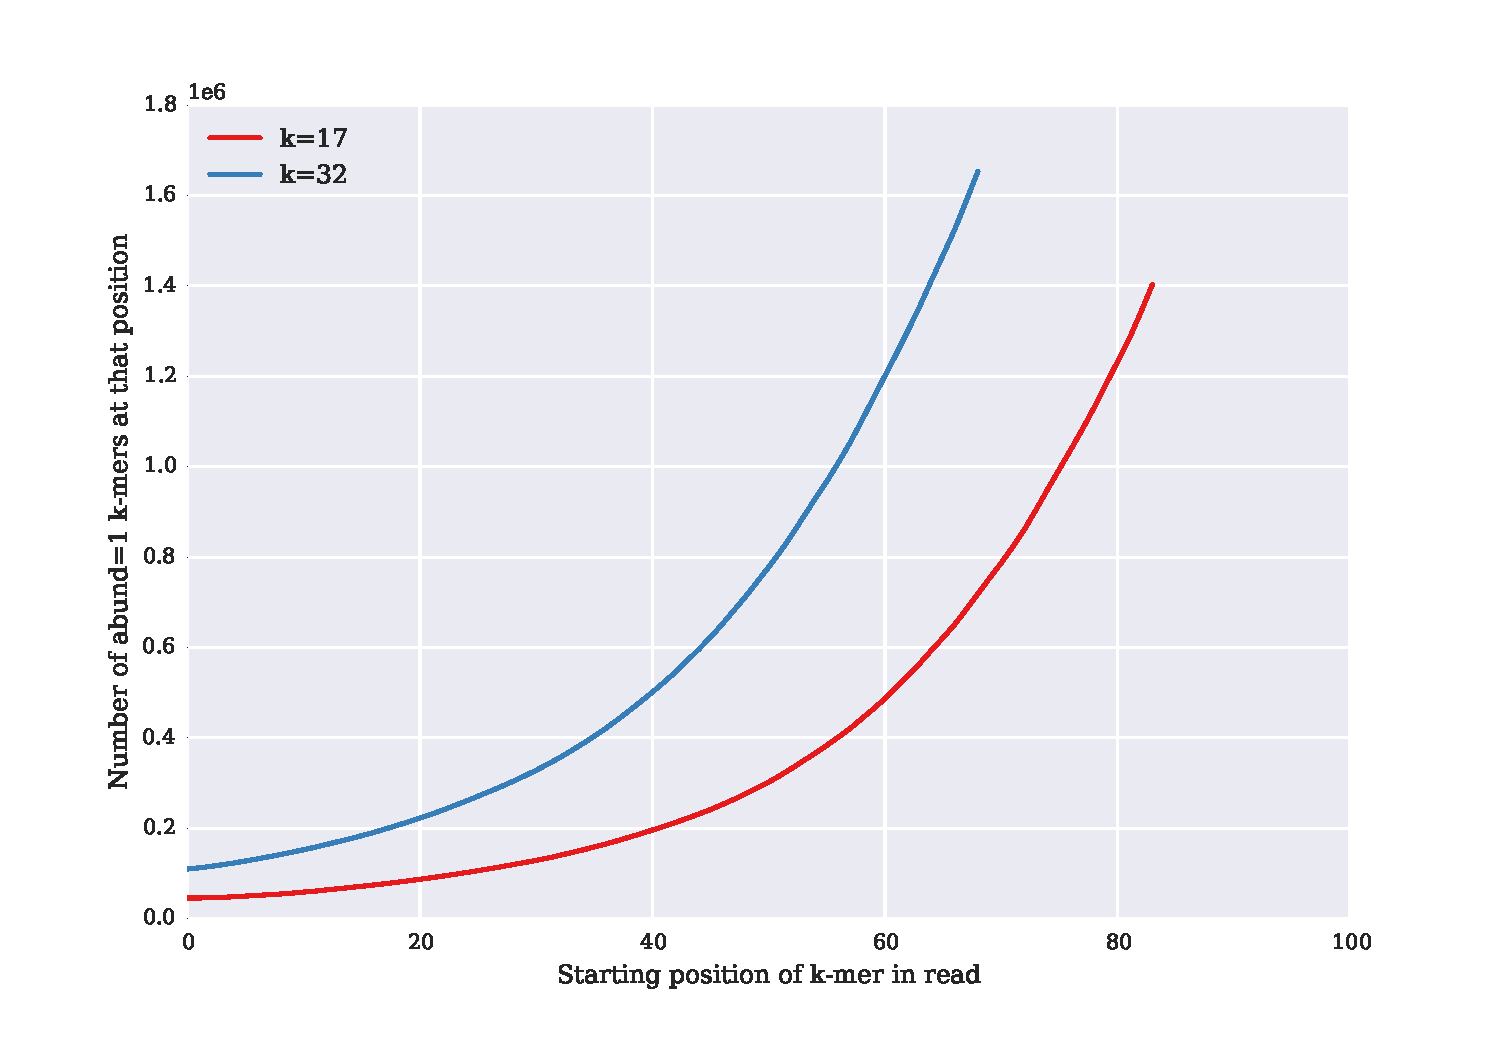
\includegraphics[width=5in]{./figures/figure7_perc_unique_pos}}
\caption{\bf Number of unique k-mers (y axis) by starting position within read
(x axis) in an untrimmed {\em E. coli} 100-bp Illumina shotgun data set, for
k=17 and k=32.  The increasing numbers of unique k-mers are a sign of the
increasing sequencing error towards the 3' end of reads.  Note that there are
only 69 starting positions for 32-mers in a 100 base read.}
\label{fig:perc_unique_pos} \end{figure}



In Figure \ref{fig:perc_unique_pos}, we use khmer to examine the sequencing
error pattern of a 5m-read subset of an Illumina reads data set from
single-colony sequencing of {\em E. coli} \cite{pubmed21926975}.  The high rate
of occurrence of unique k-mers close to the 3' end of reads is due to the
increased sequencing error rate at the 3' end of reads.


The results above demonstrated that the newly developed 
k-mer counting approach can be integrated successfully to do effective error 
analysis. This is an application where the counting error of the Count-Min Sketch approach
used by khmer may be particularly tolerable: it will never falsely
call a high-abundance k-mer as low-abundance because khmer never
underestimates counts.



\subsection{A semi-streaming algorithm can be used for error analysis}



As shown above, k-mer spectral error detection, trimming, and correction approaches
are typically implemented as a two-pass offline algorithm, , in which
k-mer counts are collected in a first pass and then reads are
analyzed in a second pass.  While several algorithms that run in
sublinear memory do exist (e.g., Lighter \cite{lighter}), these are
still offline algorithms that require two or more passes across
the data.



In high coverage data sets it is possible to implement a more
algorithmically efficient approach, by detecting reads that are high
coverage in the context of reads previously encountered in the same
pass of the data. 
Shotgun sequencing oversamples most regions -- for example, for a 100x
coverage genomic data set, we would expect 50\% or more of the genome
to be represented by more than 100 reads.  This is a consequence of
the Poisson-random sampling that underlies shotgun sequencing
\cite{waterman}.  This oversampling provides an opportunity, however:
if we regard the read data set as a stream of incoming data randomly
sampled from a pool of molecules, high-abundance species or
subsequences within the pool will be more highly sampled in the stream
than others, and will thus generally appear earlier in the stream.
For example, in mRNAseq, highly expressed transcripts should almost
always be sampled much more frequently than low-expressed transcripts,
and so more reads from highly expressed transcripts will be seen in
any given subset.With this in mind, we can develop an approach to do 
{\em semi-streaming} error analysis by detecting and
analyzing high-coverage reads {\em during} the first pass. 

We implemented this by integrating k-mer spectral
error analysis directly into the digital normalization algorithm.
As digital normalization, here we
still use the median k-mer abundance of the k-mers in a read to
estimate that read's abundance \cite{Brown2012}; crucially, this can
be done at any point in a stream, by using the online k-mer counting
functionality of khmer to determine the abundance of k-mers seen thus
far in the stream \cite{Zhang2014}. 


\begin{figure}[!ht]
 \centerline{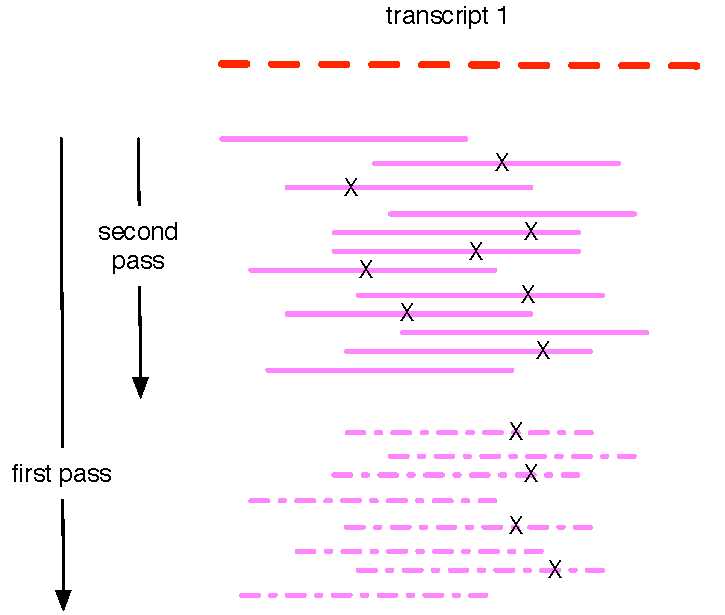
\includegraphics[width=4in]{./figures/graph-saturation}}
\caption{\bf Diagram of semi-streaming error detection. In a first pass
over the read data, reads are loaded in until the graph locus to which
they belong is saturated.  From that point on, reads are examined for
errors and not loaded into the graph.  In a second pass, only the subset
of reads loaded into the graph are examined for errors.}
\label{fig:concept}
\end{figure}

The conceptual idea is presented in Figure~\ref{fig:concept}.  On the
first pass, low-coverage reads would be incorporated into the k-mer
database with all the k-mers in them loaded into memory, and set aside for later analysis, because we can not reliably detect error, which 
is a low-abundance k-mer in a low-coverage read. 
Meanwhile, the high-coverage reads
would be analyzed for errors but would not be incorporated into the k-mer database.
This step is similar to digital normalization where the high-coverage reads are
discarded. Not loading the k-mers in those high-coverage reads decreases the
counts of those high abundance k-mers in the k-mer database a bit but this
does not affect the counts of those low abundance k-mers. So this process will
not influence the detection of errors. 
Actually the special treatment to high coverage reads also dismisses many errors in
those high coverage reads 
and this makes the detection of low abundance k-mers more accurate.

On the second pass, the set aside reads which were considered as low-coverage reads
would be checked for coverage again, and either ignored or analyzed
for errors.  Crucially, this second pass involves {\em at most}
another full pass across the data, but only when the entire data set
is below the coverage threshold; the larger the high coverage
component of the data, the smaller the fraction of the data that is
examined twice.


In Figure~\ref{fig:saturation}, we show diginorm-generated coverage
saturation curves for both real and error-free simulated reads from
{\em E. coli} MG1655.  In both cases, after the first 1m reads, the
majority of reads have an estimated coverage of 20 or higher, and
hence can be used for error analysis on the remainder of the data
encountered in the first pass.

\begin{figure}[!ht]
 \centerline{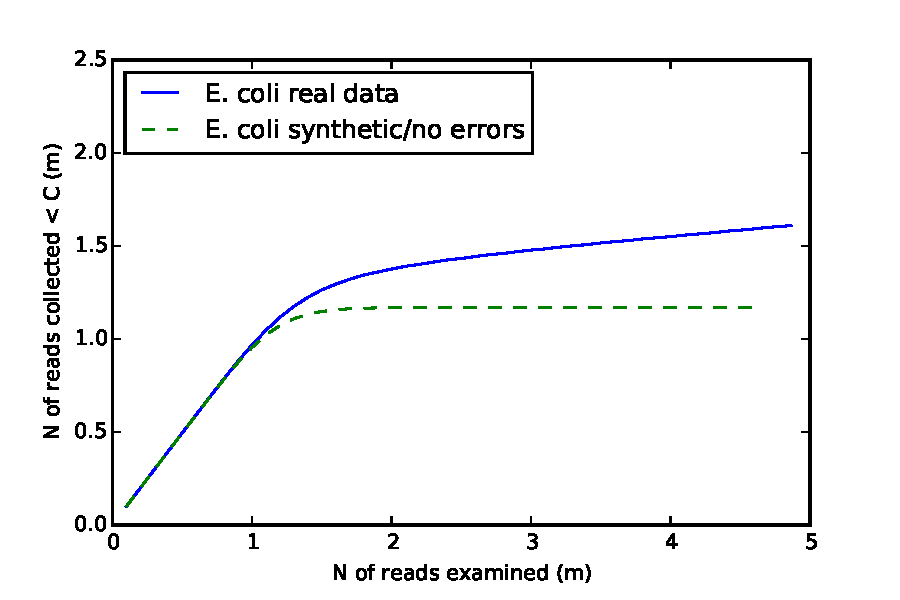
\includegraphics[width=4in]{./figures/saturation}}
\caption{\bf Saturation curve of a real and a simulated {\em E. coli}
  read data set.  Reads are collected when they have an estimated
  coverage of less than 20; in the early phase ($<$ 1m reads), almost
  all reads are collected, but by 2m reads into the data set, the
  majority of reads come from loci with an estimated sequencing depth
  of $>$ 20 and are rejected.}
\label{fig:saturation}
\end{figure}


The algorithm for the {\em semi-streaming} analysis of reads can be described as
follows:
\begin{verbatim}
for read in data:  # first pass
   if estimated_coverage(read) < C:
      count_kmers(read, k-mer_database) #
      save(read)
   else:
      analyze(read)

for read in saved_reads:   # second pass
   if estimated_coverage(read) >= C:
      analyze(read)
\end{verbatim}


As with digital normalization, a basic semi-streaming approach is very
simple to implement: with an online way to count k-mers, the algorithm
is approximately 10 lines of Python code.  The approach also requires
very few parameter choices: the only two parameters are k-mer size and
target coverage C.  However, we do not yet know how these parameters
interact with read length, error rate, or data set coverage;
systematic evaluation of parameters and the development of underlying
theory is left for future work.  In practice, we expect that
additional work will need to be done to adapt existing error
correction approaches to use the semi-streaming approach.



% 
\subsection{Semi-streaming error trimming on synthetic and real data:}

We next adapted the error detection algorithm to do semi-streaming
error trimming on synthetic or real genomic, metagenomic, and transcriptomic data. 

On the synthetic ``simple genome'' this
trimming approach eliminates 149 reads entirely and truncates another 392
reads.  Of the 100,000 bp in the simulated reads, 31,910 (31.9\%) were removed
by the trimming process.  In exchange, trimming eliminated {\em all} of the
errors, bringing the overall error rate from 0.63\% to 0.00\%.

% make mcompare5 make rcompare5
% 
For the synthetic ``simple metagenome'' we only trimmed reads with estimated coverage of 
20 or higher.  Here, of
2347 reads containing 234,700 bp, 314 reads (13.4\%) were removed and 851 reads
(36.3\%) were trimmed, discarding a total of 74,321 bases (31.7\%).  Of 1451
errors total, all but 61 were eliminated, bringing the overall per-base error
rate from 0.62\% to 0.04\%.  The simple mRNAseq data set showed similar
improvement: 83 of 568 reads were removed, and 208 were trimmed, removing
19,507 of 56,800 bases (34.34\%).  The initial error rate was 0.65\% and the
final error rate was 0.07\%. 



% ecoli-report-untrim.txt ('make ecoli-report-untrim.txt')
%posfile ecoli-reads.sam.pos: 2177509 mutated reads of 4960248; 7990149
%mutations total 496024800 bp total overall error rate: 1.610837%
%
% ecoli-report-trim.txt ('make ecoli-report-trim.txt')
%posfile ecoli-abundtrim.sam.pos: 164655 mutated reads of 4861345; 203345
%mutations total 434621201 bp total overall error rate: 0.046787%
%
% output of 'make ecoli-mapped.fq.gz.abundtrim'
% % % %
% read 4960248 reads, 496024800 bp wrote 4861345 reads, 434621201 bp removed
% 98903 reads and trimmed 2030456 reads trimmed or removed 12.38% of bases
% (61403599 total) fp rate estimated to be 0.004
% 
Applying the semi-streaming error trimming to the {\em E. coli} MG1655 data
set, we trimmed 2.0m reads and removed 50,281 reads entirely.  Of 8.0m errors,
all but 203,345 were removed, bringing the error rate from 1.49\% to 0.07\%.
Trimming discarded 53 Mbp of the original 486 Mbp (11.1\%).

% rseq_compare5.txt rseq_compare5b.txt
% 
% make podar_compare5
% 
On the mouse mRNAseq data set, semi-streaming error trimming removed 919,327
reads and trimmed 648,322 reads, removing 19.8\% of the total bases, bringing
the overall error rate from 1.59\% to 1.21\%.  When we measured only the error
rate in the high-coverage reads, trimming brought the error rate from 1.20\% to
0.42\%.  On the mock metagenome data set, 27,554 reads were removed and 171,705
reads were trimmed, removing 0.36\% of bases; this low percentage is because of
the very low coverage of most of the reads in this data set.



% ecoli-report-untrim.txt, ecoli-report-trim.txt
% rseq_compare5.txt
% rseq_compare5b.txt
% podar_
% podar_compare5b

\begin{table}
\begin{tabular}{|l|c|c|c|c|}
\hline
Data set        & pre-trim error & \% bp trim & \% reads trim & post-trim error \\
\hline
{\em E. coli}   & 1.49\%         & 11.05\%          & 41.9\%      & 0.07\% \\
\hline
mouse mRNAseq   & 1.59\%         & 13.9\%           & 19.8\%      & 1.21\% \\
(high coverage only) & 1.20\%    & 20.4\%           & 29.0\%      & 0.42\% \\
\hline
Mock metagenome & 0.31\%         & 0.4\%            & 1.1\%       & 0.28\% \\
(high coverage only) & 0.16\%    & 1.4\%            & 3.5\%       & 0.07\% \\
\hline
\end{tabular}

\caption{{\bf A summary of trimming statistics for semi-streaming
    error trimming.  Error rates before and after trimming were
    estimated by mapping. ``High coverage'' numbers refer to the
    subset of reads with $C \geq 20$ that were subject to analysis.}}
\label{tab:trimming}
\end{table}



% cmouse-compare5-post.txt  cpodar-compare5-post.txt
% cmouse-compare5-pre.txt   cpodar-compare5-pre.txt

\begin{table}
\centering
\begin{tabular}{|l|c||c|}
\hline

Data set             & mouse mRNAseq      & mock metagenome \\
\hline
Total reads          & 81.3m         & 103.2m \\
Total bp             & 6.18 Gbp      & 10.4 Gbp \\
High-coverage reads  & 74.6m         & 91.9m \\
Number of passes     & 1.18          & 1.43 \\
\% reads trim        & 25.0\%        & 11.75\% \\
\% bp trim           & 13.74\%       & 4.03\% \\
Pre-trim error rate  & 1.89\%        & 0.27\% \\
Post-trim error rate & 1.30\%        & 0.15\% \\
\hline
\end{tabular}

\caption{{\bf Results of streaming error trimming on complete data sets.
Error rates before and after trimming were estimated by mapping.}}
\label{tab:full_trimming}
\end{table}


In practice, the space and time performance of both digital normalization and
the generalized streaming approach presented here depend on specific details of
the data set under analysis and the precise implementation of the coverage
estimator. While our intention in this paper is to demonstrate the general
streaming approach, we note that even our naive implementation for e.g.
streaming trimming is useful and can be applied to very large data sets.  For
high coverage data, we can efficiently error-trim 10s of millions of reads in
both sublinear memory and fewer than two passes across the data.  In
Table~\ref{tab:full_trimming}, we show the summary statistics for streaming
error trimming of the full mouse mRNAseq and mock metagenome data; in contrast
to the smaller subsets used previously (see Table~\ref{tab:trimming}), when we
consider the full data sets the majority of reads are examined only once (see
``Number of passes'', Table~\ref{tab:full_trimming}).


The implementation of semi-streaming error trimming used here is
somewhat inefficient, and relies on redundantly storing all of the
reads needed for the second pass on disk during the first pass.  In
the worst case, where all reads are low coverage, a complete copy of
the data set may need to be stored on disk!  This is an area for
future improvement.  However, when we look at full data sets, fewer
than half the reads are examined twice (see Number of passes,
Table~\ref{tab:full_trimming}).




\subsection{Semi-streaming Illumina error rates and error profiles analysis}

\begin{figure}[!ht]
 \centerline{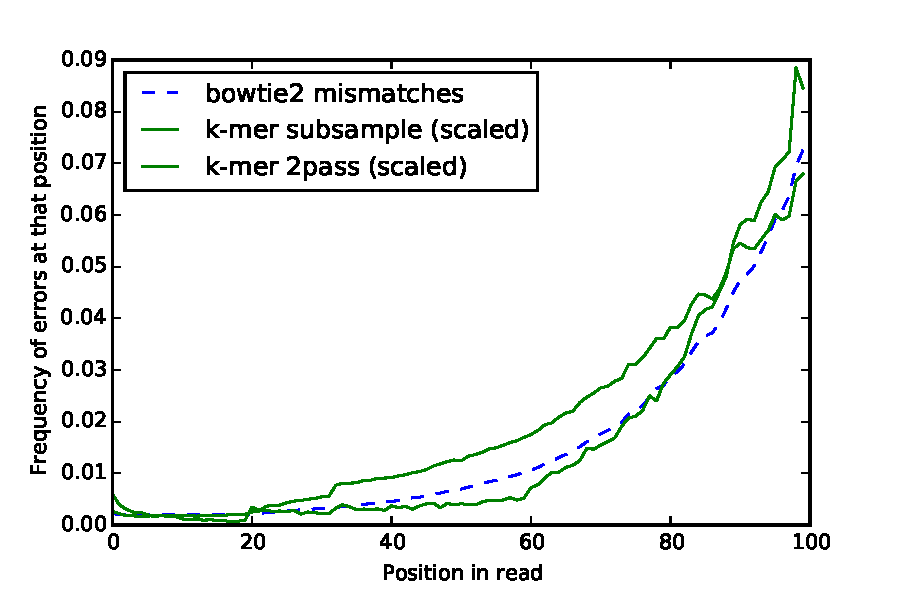
\includegraphics[width=4in]{./figures/ecoli-errhist}}
\caption{{\bf Error spectrum of reads in the {\em E. coli} data
    set. The sublinear k-mer spectrum analysis is calculated based on
    saturation of a fraction of the data set, while the two-pass
    spectral analysis uses all of the data.  bowtie2 mismatches are
    based on all mapped reads.  The y values for the k-mer spectral
    analyses are scaled by a factor of four for ease of comparison.}}
\label{fig:ecoli_err}
\end{figure}

\begin{figure}[!ht]
 \centerline{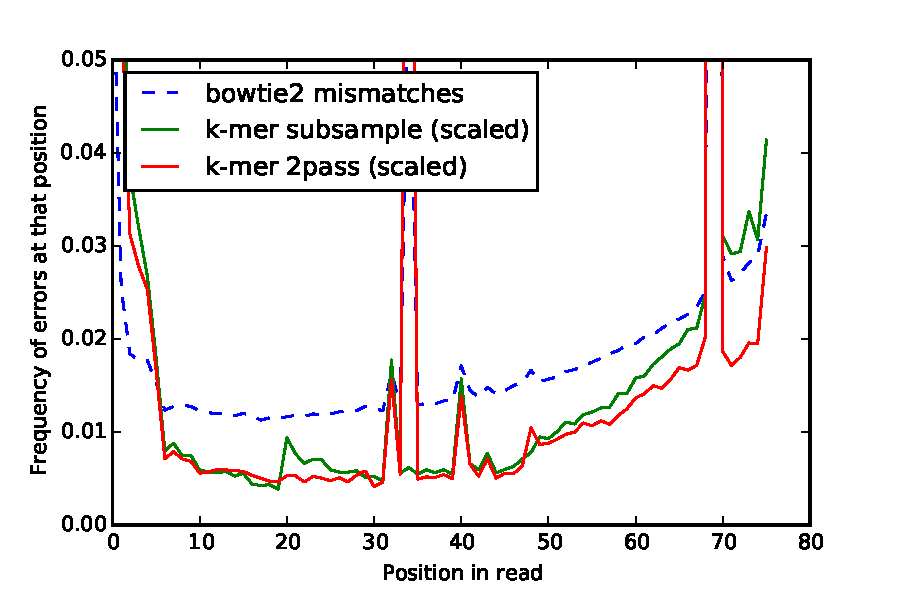
\includegraphics[width=4in]{./figures/rseq-errhist}}
\caption{{\bf Error spectrum of reads in the mouse RNAseq data set.
    The sublinear k-mer spectrum analysis is calculated based on
    saturation of a fraction of the data set, while the two-pass
    spectral analysis uses all of the data, and bowtie2 mismatches are
    based on all mapped reads.  The peak of errors at position 34 in
    the bowtie2 mapping reflects errors that in the first part of the
    data set are called as Ns, and hence are ignored by the sublinear
    error analysis; see text for details. Note, the bowtie2 mismatch
    rates are larger than the spectral rates, so for ease of
    comparison the y values for the k-mer spectral analyses are scaled
    by a factor of four.}}
\label{fig:rseq_err}
\end{figure}



We can adapt the streaming approaches above to efficiently provide estimates
for {\em subsets} of the data.  The basic idea is to consume reads until some
reads have saturated, and then to calculate error rates for new reads from the
saturated loci in the graph.  This can be done in one pass for data sets with
sufficiently high coverage data: as shown above (Figure~\ref{fig:saturation}),
in some data sets, most of the reads will have sufficient coverage to call
errors by the time 20\% of the data set has been consumed.

Using the same error detection code as above, we implemented a sublinear
memory/sublinear time algorithm that collects reads until some regions have
reached 20x coverage, or 200,000 reads have surpassed a coverage of 10x (see
Methods for details).  In either case, all reads at or above a coverage of 10
are analyzed for errors, with a trusted k-mer cutoff of 3.  In
Figure~\ref{fig:ecoli_err} and Figure~\ref{fig:rseq_err} we show the resulting
error profiles for the {\em E. coli} and mouse RNAseq data sets, compared with
the profile obtained by examining the locations of mismatches to the
references. We also show the error profile obtained with the full two-pass
approach (using digital normalization and then error detection as above) for
comparison.

In the {\em E. coli} data set (Figure~\ref{fig:ecoli_err}), we see the increase
in error rate towards the 3' end of the gene that is characteristic of Illumina
sequencing \cite{biases}.  All three error profiles agree in shape (Pearson's
correlation of 0.99 between each pair) although they are offset considerably in
absolute magnitude. The k-mer error profile was calculated from the first
850,000 reads, but is consistent across five other subsets of the data chosen
randomly with reservoir sampling (data not shown); all five subsets had
Pearson's correlation coefficients greater than 0.99 with the bowtie2 mapping
profile and the two-pass spectral approach.

The RNAseq error profile exhibits two large spikes, one at position 34 and one
at position 69.  Both spikes appear to be genuine and correlate with large
numbers of Ns in those positions in the original data set.  The spikes are
present in the profiles derived from two-pass spectral analysis as well as the
bowtie2 mismatch calculation.  However, the sublinear approach does not detect
them when using the first 675,000 reads.  This is because of the choice of
subsample: five other subsamples, chosen randomly from the entire data set with
reservoir sampling, match the match the two-pass spectral analysis (data not
shown).  The error profiles calculated from all six subsamples with the
sublinear algorithm have a Pearson's correlation coefficient greater than 0.96
with the error profiles from the full two-pass spectral approach and the
bowtie2 mismatches.


The ability to analyze high-coverage reads without examining the
entire data set offers some intriguing possibilities.  One concrete
application that we demonstrate here is the use of high coverage reads
to infer data-set wide error characteristics for shotgun data, in a
way that is robust to the sample type \cite{drisee}.  This approach
could also be integrated directly into sequencers to assess whether
the target coverage has been obtained, and perhaps stop sequencing.
More generally, the approach of using saturating coverage to truncate
computational analysis may have application to streaming sequencing
technologies such as SMRT and Nanopore sequencing, where realtime
feedback between sequencing and sequence analysis could be useful
\cite{pacbio,nanopore}.


\section{Time and space usage of the streaming algorithm for analyzing 
short DNA sequencing reads}

As shown above, the essential idea of error analysis generally is that low-abundance
k-mers contained in a high-coverage data set typically represent
random sequencing errors. We address this problem by making use of k-mer spectra, a common
approach in which reads are treated as subpaths through a De
Bruijn graph, and errors in the reads are identified by finding
low-frequency subpaths \cite{Pevzner2001}.  


We generalize this approach by
building the graph with an online algorithm and detecting regions of
the graph saturated by observations.  These regions can then be used
for per-read analysis without necessarily examining the entire data
set.


\paragraph*{Detecting graph saturation:}
We detect graph saturation with digital normalization. The digital
normalization algorithm is, in Python pseudocode:
\begin{verbatim}
for read in data:
   if coverage(read, table) < DESIRED:
      add_read_to_graph(read, graph)
      analyze(read)
\end{verbatim}
This is a single-pass algorithm that can be implemented in fixed space
using a Count-Min Sketch to store the De Bruijn graph necessary for
coverage estimation \cite{Pell2012, Zhang2014}.  For any
error-containing data set with coverage greater than {\tt DESIRED},
the graph requires space less than the size of the input - typically
space sublinear in the data size, for any fixed-size source text (see
Figure~\ref{fig:saturation} and \cite{Zhang2014}).

The digital normalization algorithm was developed as a {\em filter},
in which the reads are passed on to another program (such as a {\em
  de novo} assembler) for further analysis -- these later analyses are
typically based on multi-pass, heavyweight algorithms.  Here, digital
normalization is performing lossy compression, reducing the number of
error-containing sentences while attempting to retain the structure of
the De Bruijn graph \cite{Brown2012, Zhang2014, Lowe2015}.  This reliance
on a post-normalization heavyweight analysis step limits the
applicability of digital normalization and presents challenges in the
analysis of extremely large data sets, which motivated this work.

\paragraph*{Semi-streaming analysis:} The algorithm for {\em semi-streaming} analysis of reads is as
follows:
\begin{verbatim}
for read in data:  # first pass
   if coverage(read, graph) < DESIRED:
      add_read_to_graph(read, graph)
      save(read)
   else:
      analyze(read)

for read in saved_reads:   # second pass
   if coverage(read, graph) >= DESIRED:
      analyze(read)
\end{verbatim}
Here, the space used for the graph remains identical to the digital
normalization algorithm and is typically sublinear in space for high
coverage data sets, but the algorithm is no longer single-pass, and
requires re-examining some subset of the input data in a second pass.
In the worst case scenario, with an undersampled source text (or
randomly generated sentences), this is a fully offline two-pass
approach that requires re-examining {\em all} of the input data for
the second pass.  In practice, most real data sets will require fewer
than two passes: graphically, any deviation from the identity line in
a saturation analysis as in Figure~\ref{fig:saturation} yields a
few-pass algorithm.


\section{Conclusion}



Shotgun DNA sequencing generates data as a stream
of items representing sentences (``reads'') randomly sampled from a
larger text, with replacement. There are several distinct features of this kind
of stream-like data.
 The first is that important details of the source text,
such as its size and statistical composition, may be completely
unknown; that is, often the reads themselves are the most specific
information we have about the source text.  Second, the source text
may be incompletely sampled by the reads, and whether or not it is
completely sampled may not be known in advance.  And third, read
data sets are typically stored on disk, at least in current
implementations; our goal is to identify more efficient approaches to
examining these data sets without necessarily moving to a pure
streaming model, which allows us to make use of the {\em
  semi-streaming} paradigm introduced by Feigenbaum et
al. \cite{Feigenbaum2005}.

 In this chapter, we discussed our solutions to
two primary problems. One is to efficiently distill the non-redundant informaiton
from the streaming to reduce the size of data finally without losing much important 
information. The other one is to
efficiently identify the locations of errors in these reads by
finding differences with respect to the (unknown) source text. Both solutions 
are based on a novel approach to use median k-mer count in a read to estimate
sequencing depth without a reference assembly, which will also be the foundation
of the IGS based diversity analysis method discussed in the next chapter.

Streaming represents the future of big data. 
This kind of problems we are dealing with is not only critically important to 
a better understanding of the exploding big biological data, but also a 
gateway to a larger set of interesting domain problems
dealing with big data, like estimating the true abundance of the 
sentences in the larger text or detecting evil traffic in the internet data
stream.






\section{Data}

The code and detailed instruction used to generate all of the results in this chapter is available at
github.com/ged-lab/2012-paper-diginorm/ and 
http://github.com/ged-lab/2014-streaming/. 

\subsection{Data sets used for digital normalization}

The {\em E. coli}, {\em S. aureus}, and {\em Deltaproteobacteria} data sets
were taken from Chitsaz et al. \cite{pubmed21926975}, and downloaded from
bix.ucsd.edu/projects/singlecell/.  The mouse data set was published by
Grabherr et al. \cite{pubmed21572440} and downloaded from
trinityrnaseq.sf.net/.  All data sets were used without modification. The
complete assemblies, both pre- and post-normalization, for the {\em E. coli},
{\em S. aureus}, the uncultured {\em Deltaproteobacteria}, mouse, and yeast
data sets are available from ged.msu.edu/papers/2012-diginorm/.

The simulated genome and transcriptome were generated from a uniform AT/CG
distribution.  The genome consisted of a single chromosome 400,000 bases in
length, while the transcriptome consisted of 100 transcripts of length 500.
100-base reads were generated uniformly from the genome to an estimated
coverage of 200x, with a random 1\% per-base error.  For the transcriptome, 1
million reads of length 100 were generated from the transcriptome at relative
expression levels of 10, 100, and 1000, with transcripts assigned randomly with
equal probability to each expression group; these reads also had a 1\% per-base
error.


\subsection{Synthetic data sets used for error analysis}

We computationally constructed three small short-read DNA data sets for initial
exploration of ideas.  All synthetic sequences have equiprobable A/C/G/T.  All
synthetic reads are 100bp long and were sampled with 1\% error.  The ``simple
genome'' data set consists of 1000 reads chosen uniformly from a 1 kb randomly
constructed genome. The ``simple transcriptome'' data set consists of 568 reads
chosen uniformly from synthetic transcripts containing different subsets of
four 250-base exons, with expression levels varying by a factor of 30 from
minimum to maximum.  The ``simple metagenome'' data set consists of reads
sampled from three different 500 bp sequences, across 30 fold variation in
abundance.  In all three cases, the errors during read sampling were recorded
for comparison with predictions.

\subsection{Real data sets used for error analysis}

We used three shotgun Illumina data sets: a genomic data set from {\em E.
coli}, a mRNAseq data set from {\em Mus musculus}, and a mock community
metagenome.  For {\em E. coli}, we took a 5m read subset of ERA000206 from
\cite{chitsaz}.  For mRNAseq, we used a 10m read subset of GSE29209 from
\cite{trinityrna}.  For the mock metagenome, we used a 20m read subset of
SRR606249 from \cite{podar}.  Prior to analysis, we eliminated any read with an
'N' in it and filtered the reads by mapping to the known references, yielding
the read numbers in Table~\ref{tab:data}.


\chapter{A framework for diversity analysis of whole shotgun metagenomic reads data}



\section{Introduction}



Here we propose a novel concept - IGS (informative genomic 
segment) and use IGS as a replacement of OTUs to be the basic unit for 
diversity analysis of whole shotgun metagenomics data sets. IGSs represent the 
unique information in a metagenomics data set and the abundance of IGSs in 
different samples can be retrieved by the reads coverage through an efficient 
k-mer counting method, which was discussed in the previous two chapters.
This samples-by-IGS abundance data matrix is a promising
replacement of samples-by-OTU data matrix used in 16S rRNA based analysis and 
many existing statistical methods can be applied to work on the samples-by-IGS 
data matrix to investigate the diversity. We applied the IGS-based method to 
several simulated data sets and several real metagenomic data sets from samples
like human microbiome, sea water and soil. The results of beta diversity analysis
showed that the samples were clustered with comparable or better accuracy than 
existing alignment-based method. The results of alpha diversity analysis 
showed this was a promising new approach to estimate the metagenome size.
Since this method is totally binning-free, 
assembly-free, annotation-free, reference-free, it is specifically promising 
to deal with the highly diverse samples, while we are facing large amount of 
``dark matters'' in it, like soil.



\section{The concept of IGS(informational genomic segment)}

In classic ecology dealing with macroorganisms, diversity measurement is based 
on the concept of species. For 16S rRNA amplicon metagenomics data set, it is 
based on the concept of OTUs. While the concept of OTUs can be used to analyze
large shotgun metagenomics data set, normally assembly, binning and annotation
are required before doing diversity analysis. However for many metagenomics 
project these are difficult
tasks, lacking of necessary reference genome or being computationally
expensive. So we are interested in finding an approach to bypass the difficult
tasks like assembly, binning, annotation and use the raw reads to make the 
diversity analysis of large shotgun whole genome metagenomic data possible. 

We began such efforts by proposing that
 the concept of k-mer (a DNA segment with the length of k) could be used as the 
 basic unit to measure
the diversity. K-mers can be considered as the atom of information in DNA 
sequences. One of the composition-based approaches to binning is to use the 
k-mers as the signatures.\cite{Alneberg2014} \cite{Imelfort2014} Suppose the sizes of microbial genomes are similar and
 the difference between genomic content of microbial genomes is similar, the 
number of distinct k-mers in the sequence data set correlates to the number of 
species in a sample. However, because of sequencing error, which is unavoidable
 due to the limit of sequencing technology, this k-mer based analysis doe not 
work well. One sequencing error on a read will generate at most k erroneous 
k-mers. In metagenomics data set, especially with high coverage, most of the 
distinct observed k-mers are from sequencing errors.
%add citation about k-mer based diversity analysis ,entropy...
% add some results /figures

Next we shifted the focus from k-mers onto the upper level - reads. 
In previous chapter, we have discussed a novel approach to use median k-mer 
count in a read to estimate
sequencing depth without a reference assembly, based on which the framework for
streaming analysis of short DNA sequencing reads was developed.
It also offers a novel way to distill information from reads by reducing the
 bad effect of sequencing errors so that we can use those informative reads to 
measure the microbial diversity. We term those informative reads as 
IGSs(informative genomic segments), which can be considered as segments of DNA 
on a microbial genome. Those IGSs should be different enough to represent the 
abstract information a genome contains. Suppose microbial genomes contain 
similar number of those IGSs, as they contain similar number of distinct 
k-mers, the number of IGSs will correlate with the species richness in a 
sample, and the abundance distribution of IGSs will be related to species 
evenness in a sample. Furthermore, we can get the abundance of the IGSs across
different samples. Many classic diversity estimation methods based on OTUs 
 described in the literature review chapter can be applied to estimate 
 the diversity of IGSs 
and the diversity of actual species subsequently.


% need expanding
For alpha diversity, we can generate a list of IGSs and the respective 
abundance in a sample. Then existing estimators like Chao's can be applied to 
estimate the total number of IGSs in the sample. Rarefaction curve based on the
number of IGSs can also be generated. 

% need expand the discussion from IGS in one sample to IGS in different samples.
For beta diversity, we can generate a samples-by-IGS data matrix from the
abundance of IGSs across samples, as a replacement of samples-by-OTU data 
matrix in OTU-based analysis and samples-by-species data matrix in traditional 
ecology. From that samples-by-IGS data matrix, we can use existing methods to 
calculate similarity/dissimilarity/distance between samples and do further 
analysis like clustering and ordination. 


\subsection{IGS(informative genomic segment) can represent the novel 
information of a genome}

Median k-mer abundance can represent sequencing depth of a read, as discussed
in last chapter.\cite{Brown2012}.
 For a sequencing reads data set with multiple species, the sequencing depth of
 a read is related to the abundance of species where the read originates from. 

% figure 1a should be marked 
The upper plot in Figure \ref{fig:reads_to_IGS} shows the abundance distribution of reads 
from 4 simulated sequencing data sets with different sequencing depth - 3 
sequencing data sets generated with different sequencing coverage(1x, 10x, 40x)
 from 3 simulated random genomes respectively and 1 combined data set with all 
the aforementioned data sets. No error is introduced in these simulated 
data sets. Obviously the reads from the three data sets can be separated by 
estimated sequencing depth. The combined data set can be considered as a 
sequencing data set with three species with different abundance.

Each point on the curve shows that there are $Y$ reads with a sequencing depth of
 $X$. In other word, for each of those $Y$ reads, there are $X-1$ other reads that 
cover the same DNA segment in a genome that single read originates. So we can 
estimate that there are $Y/X$ distinct DNA segments with reads coverage as $X$. 
We term these distinct DNA segments in species genome as 
IGSs(informative genomic segments). We can transform the upper plot in 
Figure \ref{fig:reads_to_IGS} to show the number of IGSs and their respective 
reads coverage, as 
shown in lower plot. We sum up the numbers of IGSs with 
different reads coverage for each data set and get the result as shown in 
Table \ref{table:IGSs}. The sum numbers of IGSs here essentially are the areas below each curve 
in the figure.

Even though the datasets have different sequencing depth like 10X and 40X, 
they have similar numbers of IGSs. Dataset with 1X sequencing depth has fewer 
IGSs because the depth is not enough to cover all the content of the 
genome(63.2\%). The IGSs can be seen as the
genomic segments on a genome with the length of reads.(Figure \ref{fig:IGS}  
Assume the composition of species 
genome is totally random, which is the case in the simulated data sets, the 
number of IGSs(N) in a species genome is related to the size of genome(G), 
read length(L) and k size(k), which can be denoted as

\[N =\frac{G}{L}  \]
which is the number of reads that can have a 1X coverage of the genome.
For the simulated genome with size of 1M bps, read length as 80bps, expected 
number of IGSs is 

\[1000000/80 = 12500 \], 

which is pretty close to the observed value. See Table \ref{table:IGSs}


\begin{figure}[!ht]
\centerline{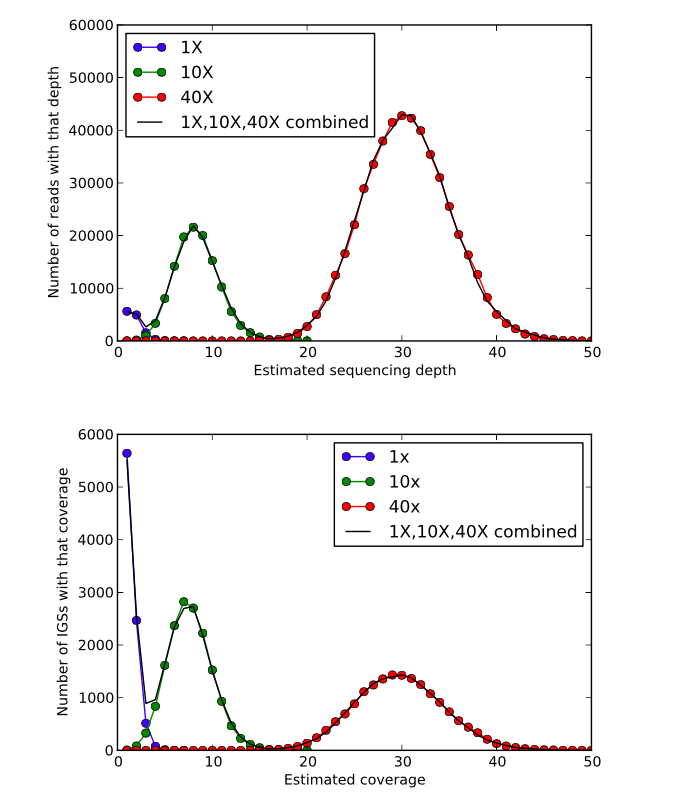
\includegraphics[width=4in]{./figures/from_reads_to_IGS.png}}
%\caption{\bf cluster of GOS samples using IGS method}
\caption{\bf from reads to IGS}
\label{fig:reads_to_IGS}
\end{figure}

\begin{table}[!ht]
\caption{
\bf{Total number of IGSs in different simulated reads data sets.}
}
\begin{tabular}{ |c | c |c| c|c| }
Data set & total number of IGSs \\
\hline \\
1X depth                   & 6419  \\
10X depth                  & 12022  \\
40X depth                  & 12371 \\
1X,10X,40X combined        & 30748 \\
\end{tabular}
\begin{flushleft}
\end{flushleft}
\label{table:IGSs}
\end{table}


\begin{figure}[!ht]
\centerline{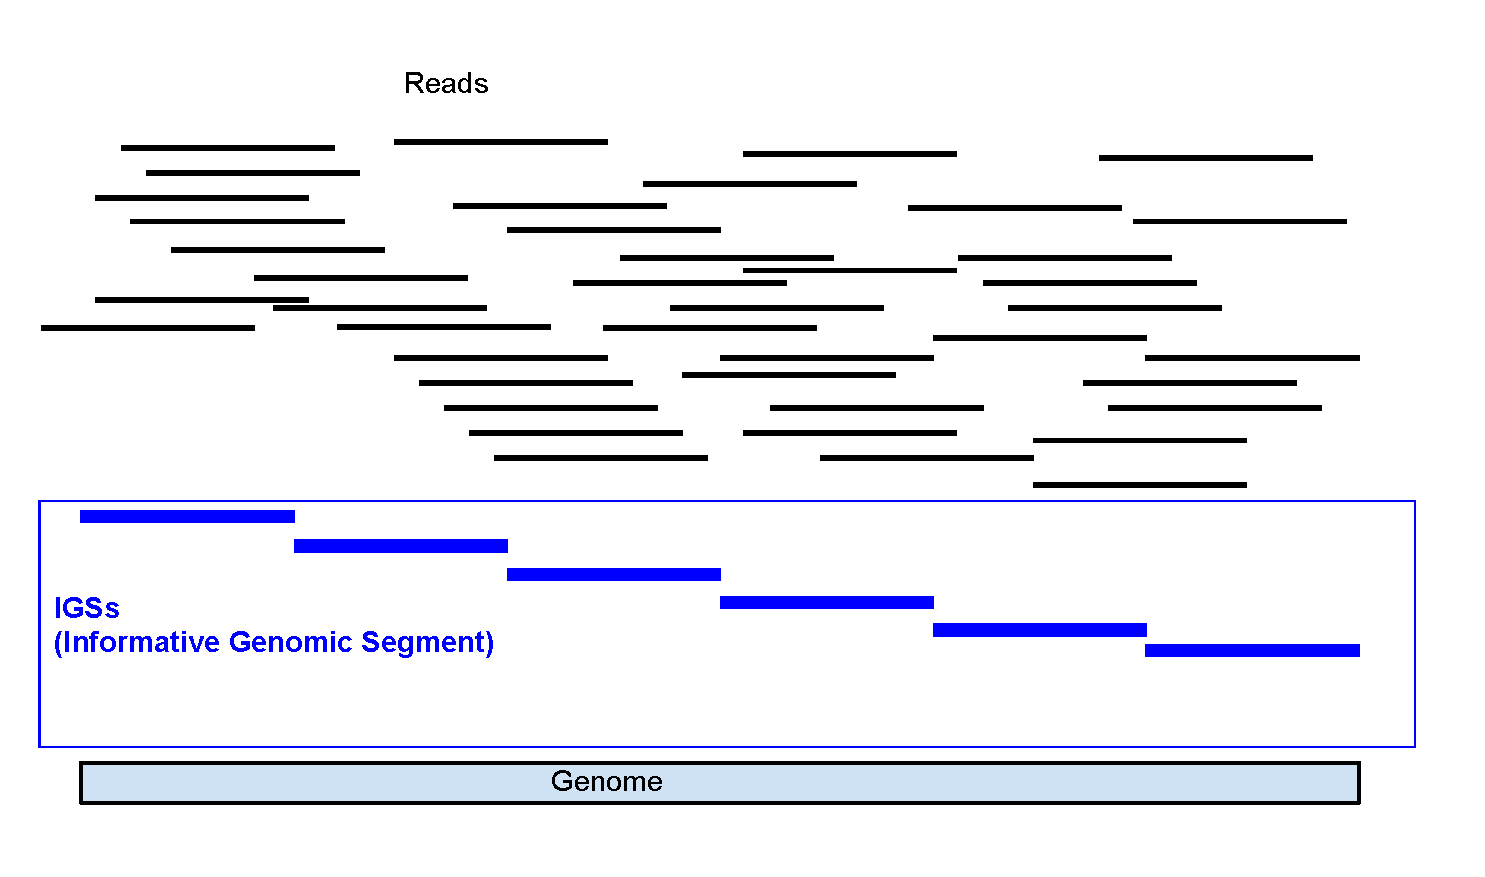
\includegraphics[width=4in]{./figures/IGSs_figure.pdf}}
\caption{\bf the concept of IGS}
\label{fig:IGS}
\end{figure}





\subsection{IGS can be used to do alpha diversity analysis}

Basically the abundance distribution of IGSs with different coverage in a 
sample data set can be acquired using the method shown above.



\begin{table}[!ht]
\caption{
\bf{coverage distribution of reads}
}
\begin{tabular}{ |c | c |c| c|c| }
coverage & number of reads \\
\hline \\
3                   & 69  \\
4                  & 96  \\
5                  & 125 \\
6        & 150 \\
...        & ... \\
\end{tabular}
\begin{flushleft}
\end{flushleft}
\label{table:coverage_reads}
\end{table}


\begin{table}[!ht]
\caption{
\bf{abundance distribution of IGSs}
}
\begin{tabular}{ |c | c |c| c|c| }
abundance & number of IGS \\
\hline \\
3                   & 23  \\
4                  & 24  \\
5                  & 25 \\
6        & 25 \\
...        & ... \\
\end{tabular}
\begin{flushleft}
\end{flushleft}
\label{table:coverage_IGS}
\end{table}

Suppose from a reads data set, the coverage distribution of reads is as 
shown in Table \ref{table:coverage_reads}. We transform this coverage distribution
of reads into abundance distribution of IGSs, as shown in Table \ref{table:coverage_IGS}.
For example, there are 23 IGSs with abundance as 3. This is calculated by dividing  
total number of reads with coverage as 3, which is 69, by the coverage 3.
Similarly there are 24 IGSs with abundance as 4. 
If we draw an analogy between IGSs and OTUs, this is like there are 23 
different OTUs with 3 reads mapped to, and 24 different OTUs with 4 reads mapped to, and so on.
Next all the different IGSs and the corresponding abundance can be listed,
as shown in Table \ref{table:list_IGS}. This list is the counterpart of an 
OTU table in OTU based diversity analysis.
With such table at hand, existing statistical methods and software 
packages can be used to investigate the alpha diversity.  


\begin{table}[!ht]
\caption{
\bf{list of IGSs with abundance information}
}
\begin{tabular}{ |c | c |c| c|c| }
IGS ID & abundance \\
\hline \\
1                   & 3  \\
1                 & 3  \\
1                  & 3 \\
...        & ... \\
23        & 3 \\
24        & 4 \\
25        & 4 \\
...        & ... \\
47        & 4 \\
48        & 5 \\
...        & ... \\
\end{tabular}
\begin{flushleft}
\end{flushleft}
\label{table:list_IGS}
\end{table}




\subsection{IGS can be used to do beta diversity analysis}

As in alpha diversity analysis, OTU table is also a foundation for beta 
diversity analysis. As long as we get a reliable OTU table, there are existing 
pipelines to do the beta diversity analysis. 

A typical OTU table across different samples is like this, which is also 
called samples-by-OTU data matrix.
\\
OTU\_ID Sample1\_ID Sample2\_ID Sample3\_ID\\
OTU1   3          4          2\\
OTU2   2          5          0\\
OTU3   3          1          4\\
\\
    
Like a OTU table, we hope to have the IGS table for the IGSs:
\\
    IGS\_ID SampleA SampleB SampleC SampleD\\
    IGS1   5       1       2       1\\
    IGS2   5       1       2       1\\
\\
    
    So now the problem is how we can generate a sample-by-IGS data matrix as 
    the counterpart of samples-by-OTU data matrix so many of  the existing 
    tools/methods used for OTU-based diversity can be borrowed for this kind 
    of IGS-based analysis, just as what is shown above for alpha diversity analysis.

Firstly, as how we get the coverage of a read from a sample dataset in this 
sample dataset, we can get the coverage of a read from a sample A dataset in 
another sample B dataset. We can still use the median k-mer count to represent 
the coverage. The basic idea is the same. 

Because a read must derive from a segment in the genome of some species in a 
sample, if a read R from sample A with a coverage C\_A in sample A has a 
coverage as C\_B in sample B, that means that segment of genome in sample A 
from which read R derive also exists in sample B. That genomic segment has 
a coverage as C\_A in sample A and has a coverage as C\_B in sample B. 
Roughly there should be about C\_A reads (read R should be one of them) 
in sampleA covering that genomic segment and C\_B reads in sampleB covering 
that genomic segment. Meanwhile, the C\_A reads in sampleA should all have 
a coverage as C\_B in sampleB, just like read R as one of them. Similarly,
the C\_B reads in sampleB should all have a coverage as C\_A in sampleA.

Suppose there are 6 reads in sample A, all have a coverage as 3 in sampleA, 
and have a coverage as 2 in sampleB.According to the discussion about IGS in previous section, the 6 reads cover 
2 IGSs with a coverage as 3 for each IGSs. There should be 4 reads in sampleB 
covering the exact same 2 IGSs, with a coverage as 2 in sampleB.
Now we have 2 distinct IGSs with redundancy as 3 and 2 in the two samples 
respectively. Small numbers are used in the analysis here as an example. It should
be noted that the analysis is based on large number statistically.

We can expand this example from 2 samples to 4 samples(A,B,C,D), as in the samples-
by-OTU(IGS) matrix above. If we find 10 reads in sampleA, with coverage as 5-1-2-1 in samples 
A-B-C-D respectively. (We call ``5-1-2-1'' a ``coverage  spectrum'' across samples.)
So there should be about 2 reads in sampleB, 4 reads in sampleC, 2 reads 
in sampleD, all of which have a ``coverage spectrum'' as ``5-1-2-1''. Basically 
these 18 reads altogether cover 2 distinct IGSs, which apparently exist in 
all the 4 samples. The 2 distinct IGSs has a coverage as 5,1,2,1 in the 
4 samples respectively.If we draw an analogy between IGSs and OTUs, this is like there are 2 OTUs, 
both with 5,1,2,1 reads mapped to in sample A,B,C,D respectively.

Like a OTU table, here we can have the IGS table for the two IGSs:
\\
    IGS\_ID SampleA SampleB SampleC SampleD\\
    IGS1   5       1       2       1\\
    IGS2   5       1       2       1\\
\\
    
    
    
 % should all include alpha and beta diversity results
\section{Evaluating IGS method using simulated data sets}
\subsection{Using a simple simulated data set to evaluate the IGS method}


For this experiment, firstly we create 6 synthetic samples (Sample 1-6) 
based on 9 synthetic 100K genomes (genome A-I), with different composition of species and diversity. 
(Table \ref{table:simulated_metag})For sample1, there are two species - A and B, with abundance distribution as 3:1.
The sequencing depth of all the synthetic data sets is 10X. 
As a simple experiment to demonstrate the effectiveness of the IGS based method, 
there is no sequencing error introduced in the 
synthetic reads data sets.

\begin{table}[!ht]
\caption{
\bf{6 synthetic simple metagenomes}
}
\begin{tabular}{ |c | c |c| c|c| }
sample ID & species composition & sequencing depth & abundance of species & size of metagenome (bp)\\
\hline \\
sample1        & AAAB & 10 & A:30 B:10 & 200K\\
sample2        & AABC & 10 & A:20 B:10 C:10 & 300K\\
sample3        & ABCD & 10 & A:10 B:10 C:10 D:10 & 400K\\
sample4        & ABCE & 10 & A:10 B:10 C:10 E:10 & 400K\\
sample5        & AFGH & 10 & A:10 F:10 G:10 H:10 & 400K\\
sample6        & IFGH & 10 & I:10 F:10 G:10 H:10 & 400K\\

\end{tabular}
\begin{flushleft}
\end{flushleft}
\label{table:simulated_metag}
\end{table}

To evaluate the effectiveness of alpha diversity analysis using IGS based method,
we can use statistic metric to estimate the total number of IGSs in a sample, 
which can be used to calculate the estimated genome size of a sample using the 
formula below: size of genome = number of IGS $*$ reads\_length

In this experiment, we use ACE metric since we find it is more accurate than 
Chao1, since it uses more abundance information.


\begin{table}[h]
\begin{tabular}{|l|l|l|l|l|l|}
\hline
\textbf{} & \textbf{\begin{tabular}[c]{@{}l@{}}observed \\ IGS\end{tabular}} & \textbf{ACE} & \textbf{\begin{tabular}[c]{@{}l@{}}simpson \\ evenness\end{tabular}} & \textbf{\begin{tabular}[c]{@{}l@{}}estimated \\ genome size\end{tabular}} & \textbf{\begin{tabular}[c]{@{}l@{}}real \\ genome size\end{tabular}} \\ \hline
\textbf{sample1} & 2002 & 2002.0 & 0.76 & 200200.0 & 200000 \\ \hline
\textbf{sample2} & 3038 & 3038.0 & 0.83 & 303800.0 & 300000 \\ \hline
\textbf{sample3} & 4076 & 4076.0 & 0.91 & 407600.0 & 400000 \\ \hline
\textbf{sample4} & 4078 & 4078.0 & 0.91 & 407800.0 & 400000 \\ \hline
\textbf{sample5} & 4069 & 4069.0 & 0.91 & 406900.0 & 400000 \\ \hline
\textbf{sample6} & 4087 & 4087.0 & 0.91 & 408700.0 & 400000 \\ \hline
\end{tabular}
\label{table:alpha_simulated}
\end{table}

Table \ref{table:alpha_simulated} shows the alpha diversity analysis result of the simple simulated data using IGS method. The estimated
genome sizes of the samples are close to real size. This is not surprising since for this simple experiment, 
there is no error introduced and the coverage is high (10x) to cover most of the genetic materials in the samples. 
Also the Simpson evenness shows the relative evenness of the samples correctly. 
Sample 1 is the least even with composed of two  species with abundance ratio as 1:3.
This proves the IGS method can not only analyze the richness of samples but 
also the evenness.



To evaluate the effectiveness of beta diversity analysis using IGS based method, 
we compared the dissimilarity matrix generated by IGS based method with the 
true matrix,since we know exactly the species composition of the 
simulated data set.


\begin{table}[h]
\begin{tabular}{|l|l|l|l|l|l|l|}
\hline
                  & \textbf{sample 1} & \textbf{sample2} & \textbf{sample 3} & \textbf{sample 4} & \textbf{sample 5} & \textbf{sample 6} \\ \hline
\textbf{sample 1} & 0.00              & 0.25             & 0.50              & 0.50              & 0.75              & 1.00              \\ \hline
\textbf{sample 2} & 0.25              & 0.00             & 0.25              & 0.25              & 0.75              & 1.00              \\ \hline
\textbf{sample 3} & 0.50              & 0.25             & 0.00              & 0.25              & 0.75              & 1.00              \\ \hline
\textbf{sample 4} & 0.50              & 0.25             & 0.25              & 0.00              & 0.75              & 1.00              \\ \hline
\textbf{sample 5} & 0.75              & 0.75             & 0.75              & 0.75              & 0.00              & 0.25              \\ \hline
\textbf{sample 6} & 1.00              & 1.00             & 1.00              & 1.00              & 0.25              & 0.00              \\ \hline
\end{tabular}
\caption{\bf Dissimilarity matrix between synthetic samples using Bray-curtis from species composition directly }
\label{table:simulated_real_matrix}
\end{table}

\begin{table}[h]
\begin{tabular}{|l|l|l|l|l|l|l|}
\hline
                  & \textbf{sample 1} & \textbf{sample2} & \textbf{sample 3} & \textbf{sample 4} & \textbf{sample 5} & \textbf{sample 6} \\ \hline
\textbf{sample 1} & 0.00              & 0.35             & 0.60              & 0.66              & 0.80              & 1.00              \\ \hline
\textbf{sample 2} & 0.35              & 0.00             & 0.42              & 0.51              & 0.84              & 1.00              \\ \hline
\textbf{sample 3} & 0.60              & 0.42             & 0.00              & 0.56              & 0.89              & 1.00              \\ \hline
\textbf{sample 4} & 0.66              & 0.51             & 0.56              & 0.00              & 0.89              & 1.00              \\ \hline
\textbf{sample 5} & 0.80              & 0.84             & 0.89              & 0.89              & 0.00              & 0.42              \\ \hline
\textbf{sample 6} & 1.00              & 1.00             & 1.00              & 1.00              & 0.25              & 0.00              \\ \hline
\end{tabular}
\caption{\bf Dissimilarity matrix between synthetic samples using Bray-cutis from sequencing reads using IGS method }
\label{table:simulated_matrix1}
\end{table}


The true dissimilarity matrix of the 6 simulated samples using bray-cutis 
metric from species composition directly is shown in Table \ref{table:simulated_real_matrix}.
For a simulated data set with 10x coverage and no error introduced 
(which will tell us the optimal performance of IGS method), the dissimilarity 
matrix can be calculated by using IGS method, as shown in Table 
\ref{table:simulated_matrix1}. We can see the absolute values in the matrix 
are not very close to that in the real matrix.But the relative values 
correspond to that in the real matrix well to show the relative distance 
between each pair of samples. To get a objective metric, we use 
Mantel (citing)test to calculate the correlation value between the two 
matrixes. The correlation is 0.9714, which means a very positive correlation 
between the two matrices. We are confident that the dissimilarity matrix from IGS method 
can reflect the true relationship between samples effectively.


If the matrix can reflect the real 
relationship between samples reliably, the clustering and ordination
will only be routine tasks.


\begin{figure}[!ht]
 \centerline{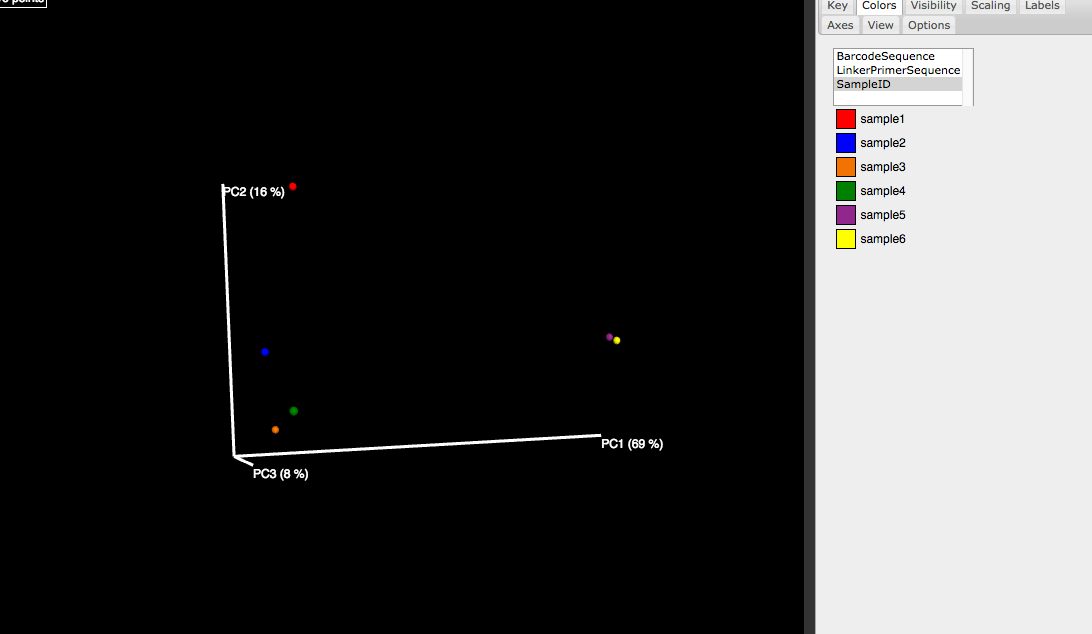
\includegraphics[width=4in]{./figures/simple_PCA_3d.png}}
\caption{\bf Ordination of the 6 synthetic samples using IGS method}
\label{fig:simple_pcoa}
\end{figure}


\begin{figure}[!ht]
 \centerline{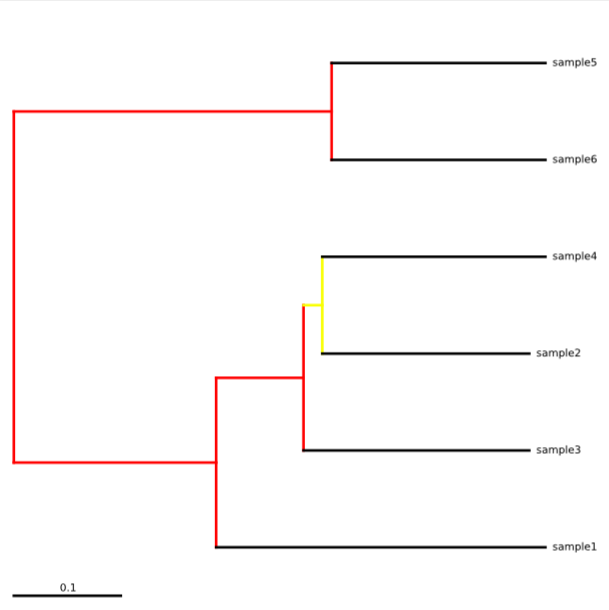
\includegraphics[width=4in]{./figures/simple_tree.png}}
\caption{\bf Clustering of the 6 synthetic samples using IGS method}
\label{fig:simple_cluster}
\end{figure}



Figure \ref{fig:simple_pcoa} and Figure \ref{fig:simple_cluster} show that 
IGS method can yield similarity between samples correctly. Sample 5 and sample 6 and very 
close to each other on the figure, which 
is true if we check the species composition of the two samples shown above.


The clustering and ordination are all from the dissimilarity matrix. 
We think comparing matrix directly makes more sense than comparing the 
clustering and ordination plots. So we will not show the clustering and 
ordination figure in other evaluation in this section. Mantel correlation will 
be used to measure the accuracy of beta diversity analysis.


These results show that the IGS method can work well to a simplest 
scenario, with high sequencing depth (10X) and no sequencing error. Next 
we will check the influence to the analysis accuracy of variable sequencing 
depth and sequencing error and introduce new ways to preprocess the data 
to decrease the influence of sequencing error. 



\subsection{Improving the accuracy of this method in real world analysis}


Previously we have shown the IGS method generally works to a simple simulated
 data set, with high sequencing depth and no sequencing error. In real world,
in many situations we have to deal with the metagenomic data sets with 
relatively low sequencing depth, like soil or sea water samples. 
Also it is a fact that all sequencing technology will generate some errors. As 
discussed in the introduction 
chapter, one of the reasons why we develop the IGS method is that 
it is expected that the IGS 
method is less prone to sequencing error based on the 
abundance counting of reads rather than k-mers, . However the effect of those factors 
jeopardizing the accuracy is still observable. 

In this section, we will analyze the effect of these factors to the accuracy of
 the IGS method and investigate the ways to reduce the effect to increase the 
accuracy of analysis.

As in last section, six synthetic samples were generated with the same species 
composition with same coverage as 10X but with different sequencing error rate (0.5\%,
 1.0\%, 1.5\%, and 0\% - no error at all).
 
To show the influence of sequencing error to accuracy of the 
analysis, we compared the richness estimation using reads with different 
sequencing error rate, as shown in Figure \ref{fig:IGS_richness_no_adjustment}. 
For data set without error (error rate = 0), the estimated size of metagenome
matches real size perfectly. With increasing error rate, the size of metagenome
is over estimated more and more seriously. This is due to several factors,which
will be discussed below. 
\begin{figure}[!ht]
 \centerline{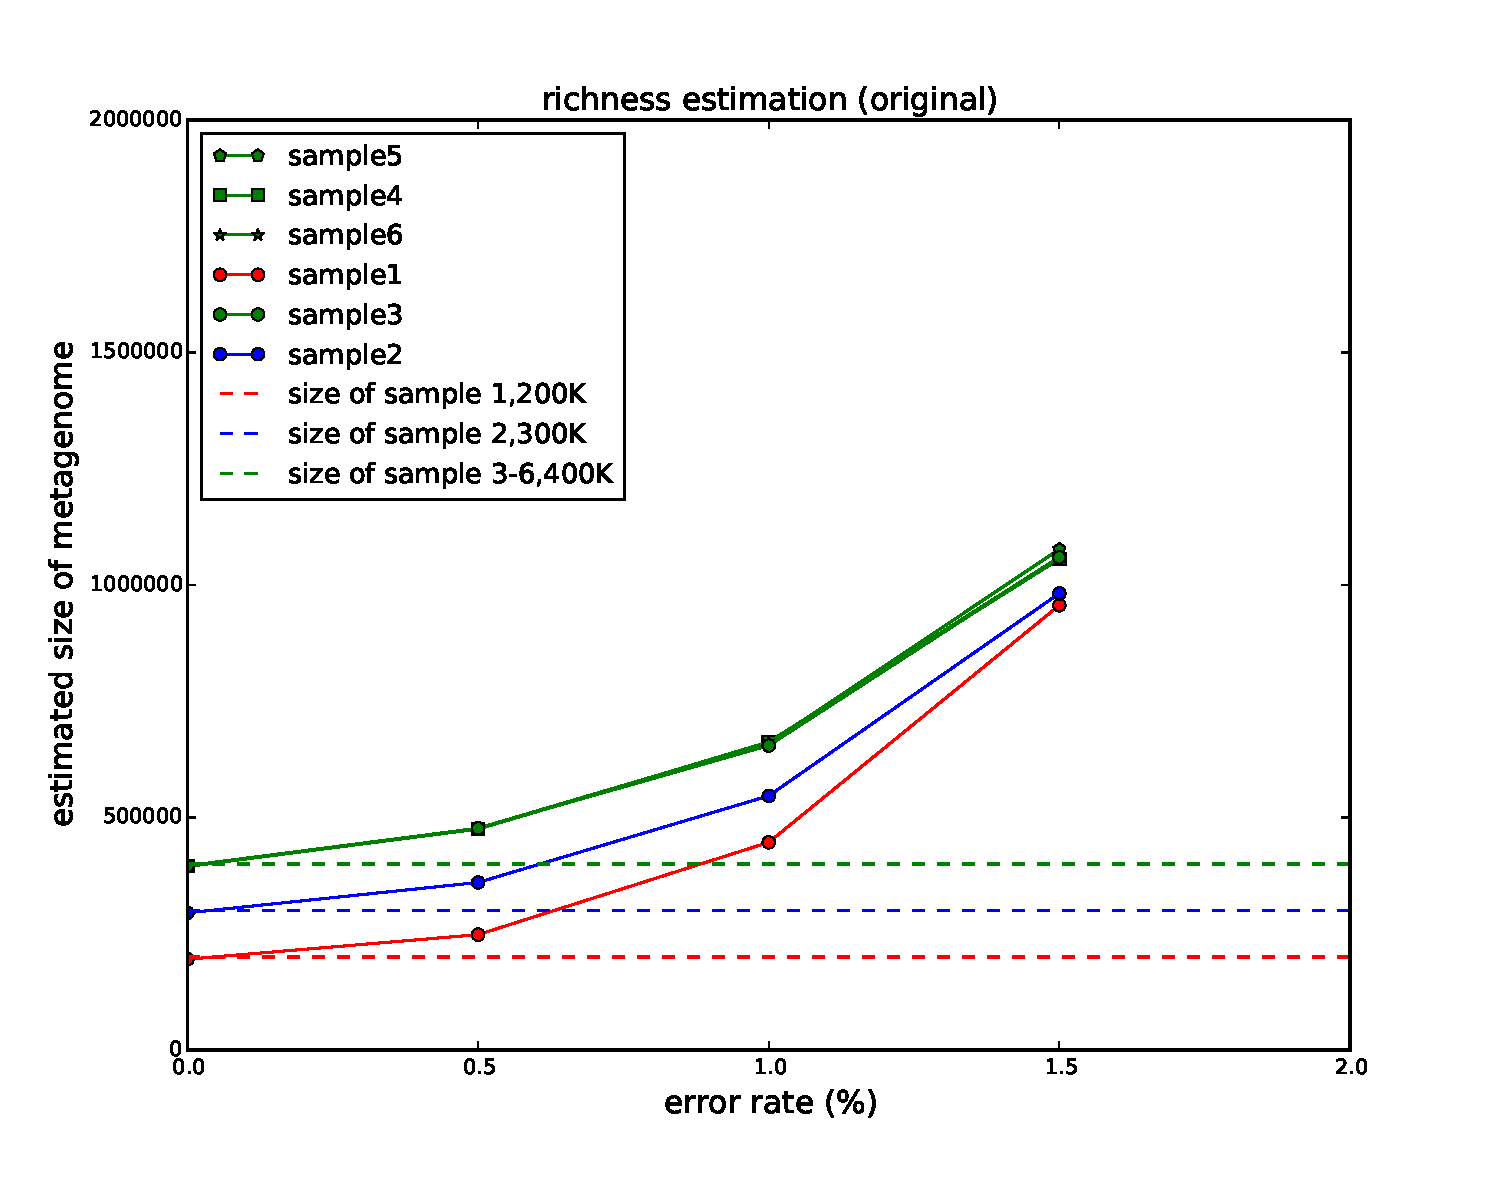
\includegraphics[width=4in]{./figures/alpha_by_error_no_adjust.pdf}}
\caption{\bf Richness estimation using IGS method without adjustment}
\label{fig:IGS_richness_no_adjustment}
\end{figure}

\begin{figure}[!ht]
 \centerline{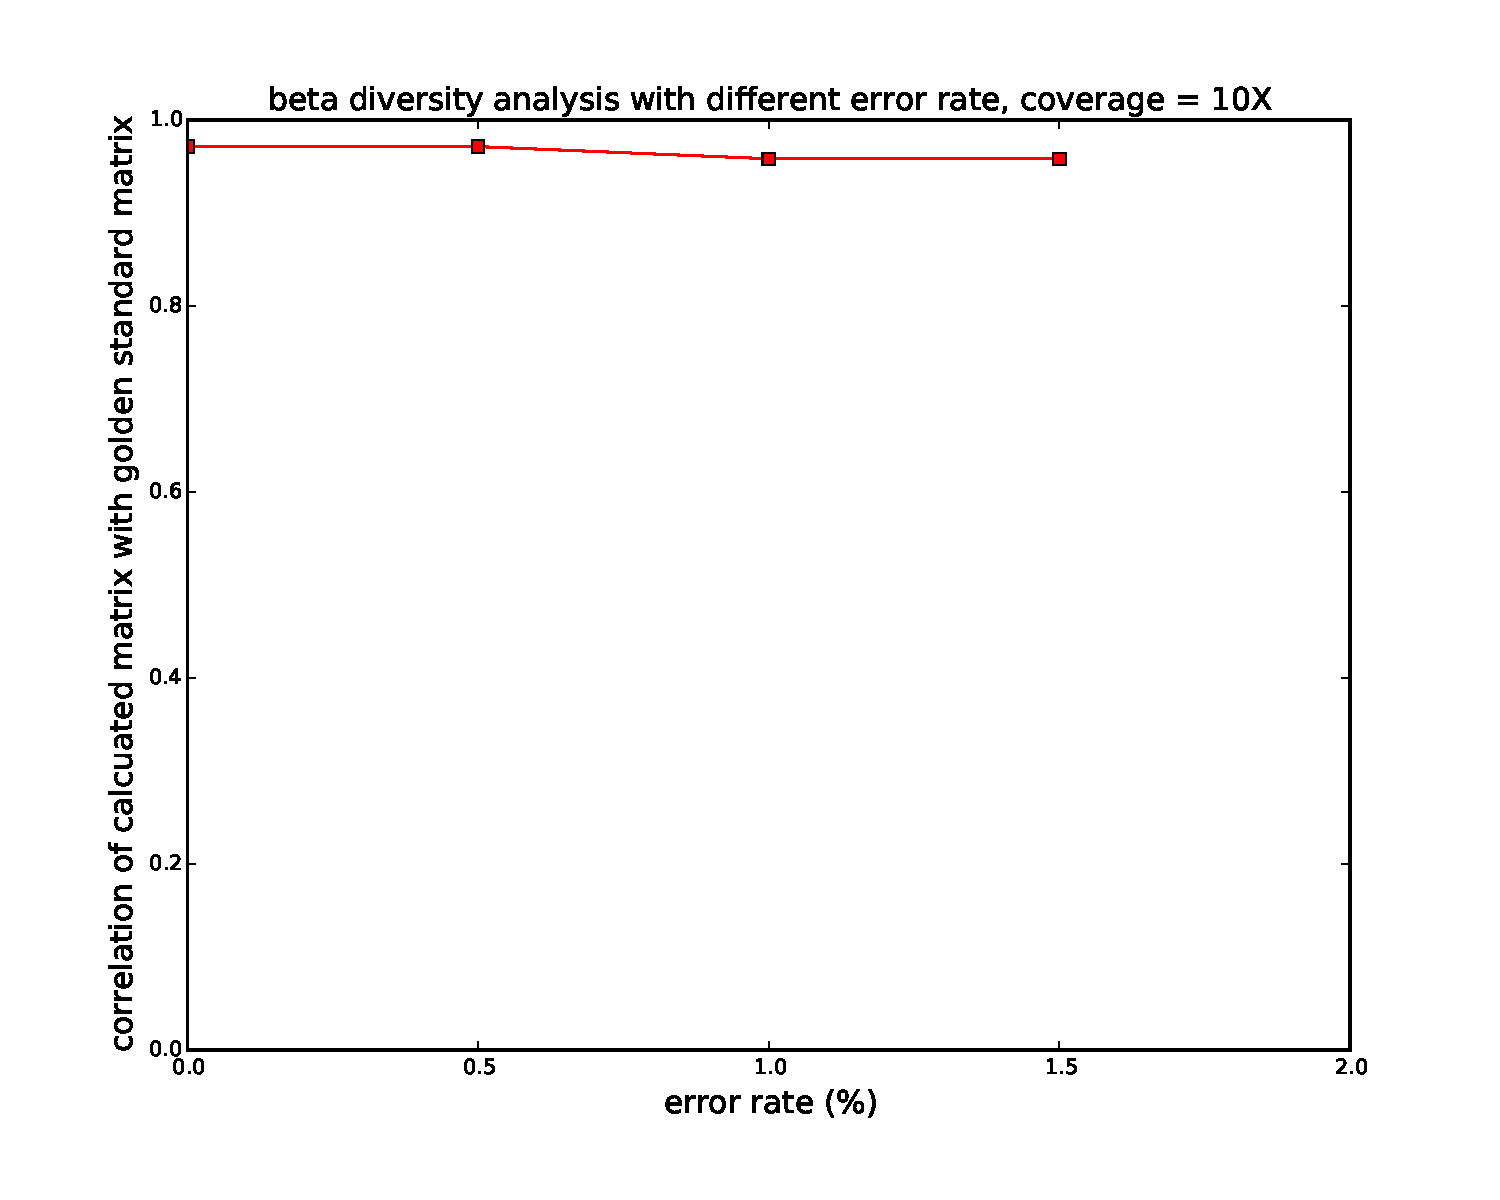
\includegraphics[width=4in]{./figures/beta_by_error.pdf}}
\caption{\bf Beta diversity analysis using IGS method without adjustment}
\label{fig:beta_no_adjustment}
\end{figure}

We also check the beta diversity analysis with different error rate and notice
that the beta diversity is less prone to increasing sequencing error rate. We 
will focus on alpha diversity in the discussion below.

\subsubsection{the effect of sequencing error to the accuracy of analysis}
The first factor to take into account is sequencing error. One sequencing error
will generate k erroneous k-mers. This is the reason why it is difficult to use
k-mer counting only to do diversity analysis, as a large proportion of k-mers
in a reads data set are erroneous, especially for low coverage reads data. As
discussed in the section about digital normalization, using median k-mer count
to retrieve the coverage of a read is less prone to sequencing error, because
sequencing error will decrease the count of some reads to 1 incorrectly, but
this does not always affect the median k-mer count. 

Take the experiment we did
previously as an example, for read length as 100bp and k as 19, one sequencing
error will affect the count of 19 k-mers at the most, two sequencing errors
will affect the count of at most 38 k-mers. The count of these k-mers will be
retrieved as 1 incorrectly, suppose it is highly impossible that an erroneous
k-mer is the same as another real k-mer in the data set accidentally, as long as
the k is large enough compared to the size of data set. So out of the 82 k-mers
in the 100bp read, at most 38 k-mers will have count as 1 incorrectly, but this
will not affect the median k-mer count, which is the count of the 41th k-mer if
ranked by count. However, if there are three or more errors in the read, the 
situation is more complicated. For 3 errors in a read, 3 to 57 k-mers
will be affected by the errors to have an incorrect count as 1. The 
distribution of the probability about the number of affected k-mers can be
acquired by a model similar to Lander-Waterman model used in genome sequencing
 theory. Here we got the distribution using simulation, as shown in Figure
\ref{fig:IGS_affected_k_kmers}. From this probability distribution, we can get
the probability that 3 errors will affect more than 40 k-mers is 0.43. In this
case, 3 errors will affect the median k-mer count of a read. We can also get 
such probability for 4 errors or more. Combining to the probability that a
certain number of errors occur in a read with a specific sequencing error rate,
which is easy to derive from binomial distribution, we can get the probability
that the coverage of a read is incorrectly assessed as 1. Still for the example
here, this probability is the probability that 3 errors occur in a read
multiplied by the probability that 3 errors will affect median k-mer count,
plus the probability that 4 errors occur in a read multiplied by the 
probability that 4 errors will affect median k-mer count,and so on.

Generally, let $P\_error(n,e,L)$ is the probability that $n$ errors occur in a 
read with length as $L$, with error rate as $e$ and $P\_effect(n,k,L)$ is the 
probability that $n$ 
errors in a read with length of $L$ affect median k-mer count. The probability 
that the coverage of a read is incorrectly assessed as 1 is 
\[\sum_{n=3}^{\infty} P\_error(n,e,L) \times P\_effect(n,k,L)  \],
and by binomial distribution,

\[P\_error(n,e,L) = f(n;L,e) = Pr(X=n) = {L \choose n}e^n(1-e)^{L-n} \] 

Practically, when $n>5$ and $e<0.015$, $P\_error(n,e,L)$ is very small, we only consider
number of errors in a read as 3, 4 and 5.

\begin{figure}[!ht]
 \centerline{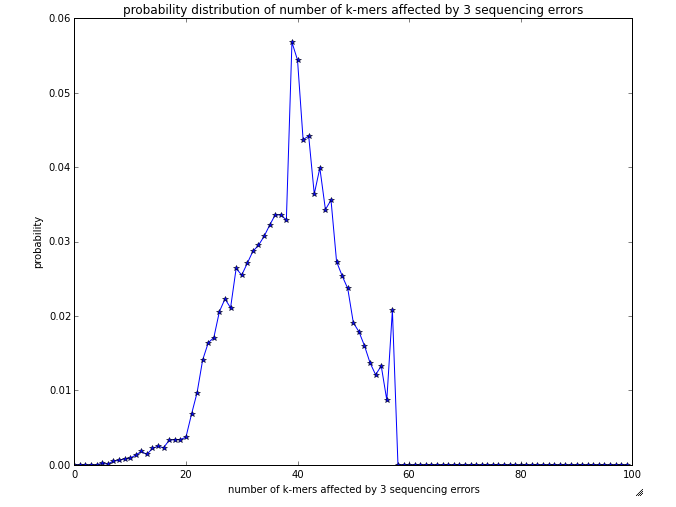
\includegraphics[width=4in]{./figures/IGS_affected_k_kmers.png}}
\caption{\bf Richness estimation using IGS method without adjustment }
\label{fig:IGS_affected_k_kmers}
\end{figure}

From the discussion above, the sequencing errors reduce the coverage of some
reads incorrectly to 1 and the probability this occurs to a read can be
estimated. So to reduce the effect of sequencing error on this aspect, we can
calculate the expected number of reads that are affected and remove those reads
from the set of reads with coverage as 1 before generating list of IGS from the
reads abundance distribution.

Also, we want to make sure 2 errors in a read will not affect median k-mer 
count, since it is more common to have 2 errors in a read practically. 
In this case, 
\[2 \times k < \lfloor \frac{L-k+1}{2}\rfloor \],
we can get $k<L/5$,basically. For $L$ as 100, $k$ will be 19, which is what we 
choose in the testing. However, the $k$ should not be too small, or the k-mers 
can not handle the information of a large data set.

Taking the sequencing error into account, we used the methods introduced above
to adjust the estimation of metagenome size of the 6 synthetic samples. The
estimation after adjustment is closer to real number, as shown in Figure
\ref{fig:IGS_richness_error_adjustment}..


\begin{figure}[!ht]
 \centerline{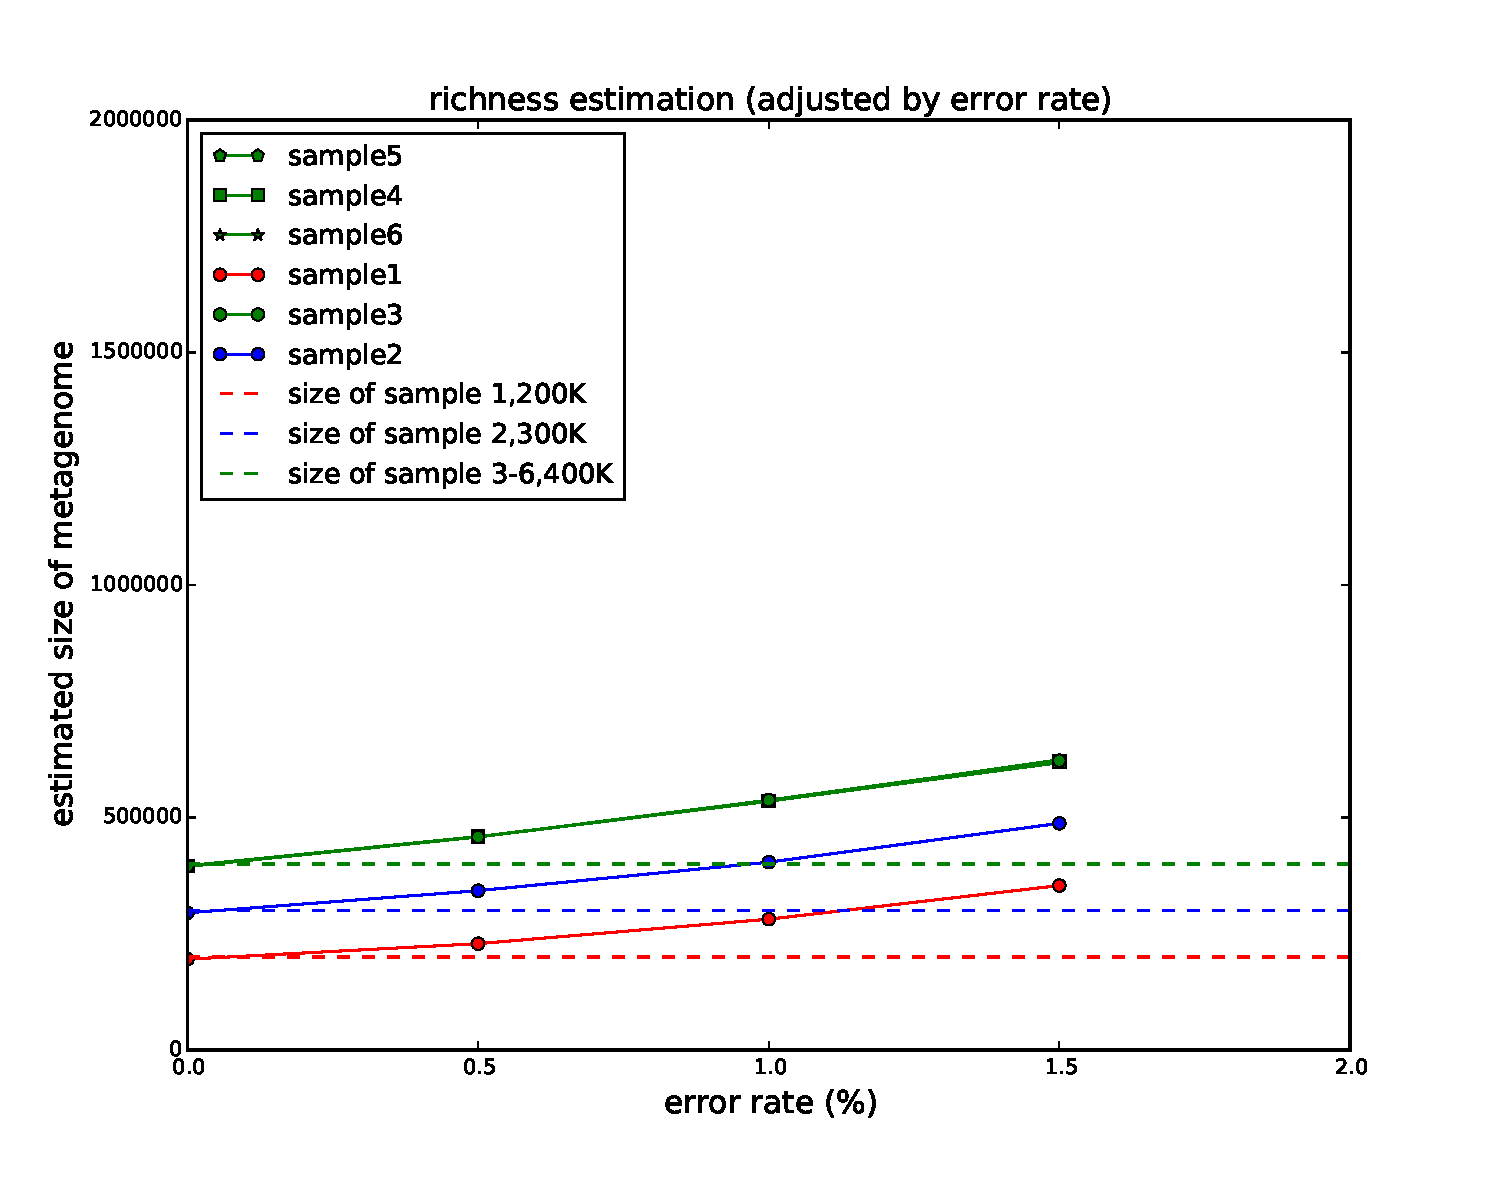
\includegraphics[width=4in]{./figures/alpha_by_error_erroronly_adjust.pdf}}
\caption{\bf Richness estimation using IGS method adjusted by sequencing error rate}
\label{fig:IGS_richness_error_adjustment}
\end{figure}

\subsubsection{the effect of collision in bloom filter to the accuracy of analysis}
As discussed in the chapter about k-mer counting, the collision in bloom filter
which we use for efficient k-mer counting will result in counting error. If the
false positive rate for a specific bloom filter we use for k-mer counting is
0.1, 10\% of the k-mers will have incorrect counts. When we use median k-mer
count to get read coverage, such incorrect count has the effect on two aspects.
On one hand, some k-mers in a read will have incorrect higher count. But if the
 false
positive rate is low, this will not affect median k-mer count. This shows the
method of using median k-mer count to get read coverage is not only less prone
to sequencing error, but also less prone to the inaccuracy characteristics of
underlying data structure. One the other hand, this inaccurate count also
affects the counts of those erroneous k-mers generated by sequencing error. For
example, 3 errors in a read affect the count of 43 k-mers, the counts for these
43 k-mers are supposed to be 1. But because of the collision in bloom filter
and the resulting incorrect k-mer counting, if the false positive rate is 0.1,
about 4 out of the 43 k-mers will have inflated count, mostly as 2. So the
combined effect of sequencing error and collision in bloom filter is that some
reads will have incorrect coverage as 1 and some reads will have incorrect as
2. We can get the percentage of total reads that will have such incorrect
coverage, using statistical model similar to that discussed in last section.
Using same example, 3 errors occur in a read, if the 3 errors affect 41-45
k-mers(with a chance of 0.20), the median k-mer count will be 2, due to the 
collision in bloom filter, while if he 3 errors affect more than 45 k-mers(with 
a chance of 0.24), the median k-mer count will be 1, purely due to sequencing 
errors. 

We did the same experiment but also adjusted the estimation according to the 
false positive rate of bloom filter and got better estimation, as shown in
Figure \ref{fig:IGS_richness_adjustment}.

With adjustment to estimation taking sequencing error and collision in bloom
filter into account, as shown in Figure \ref{fig:IGS_richness_adjustment}, the 
estimated genome size is closer to real number. With error rate as 1\%,
false positiver rate as 0.1, with 10X coverage data, the estimated genome size
is about 20-25\% more than real number. However the estimation is still 
increasing with higher
error rate. This means there are still other factors influencing this
accuracy of the estimation but we failed to take into account.


\begin{figure}[!ht]
 \centerline{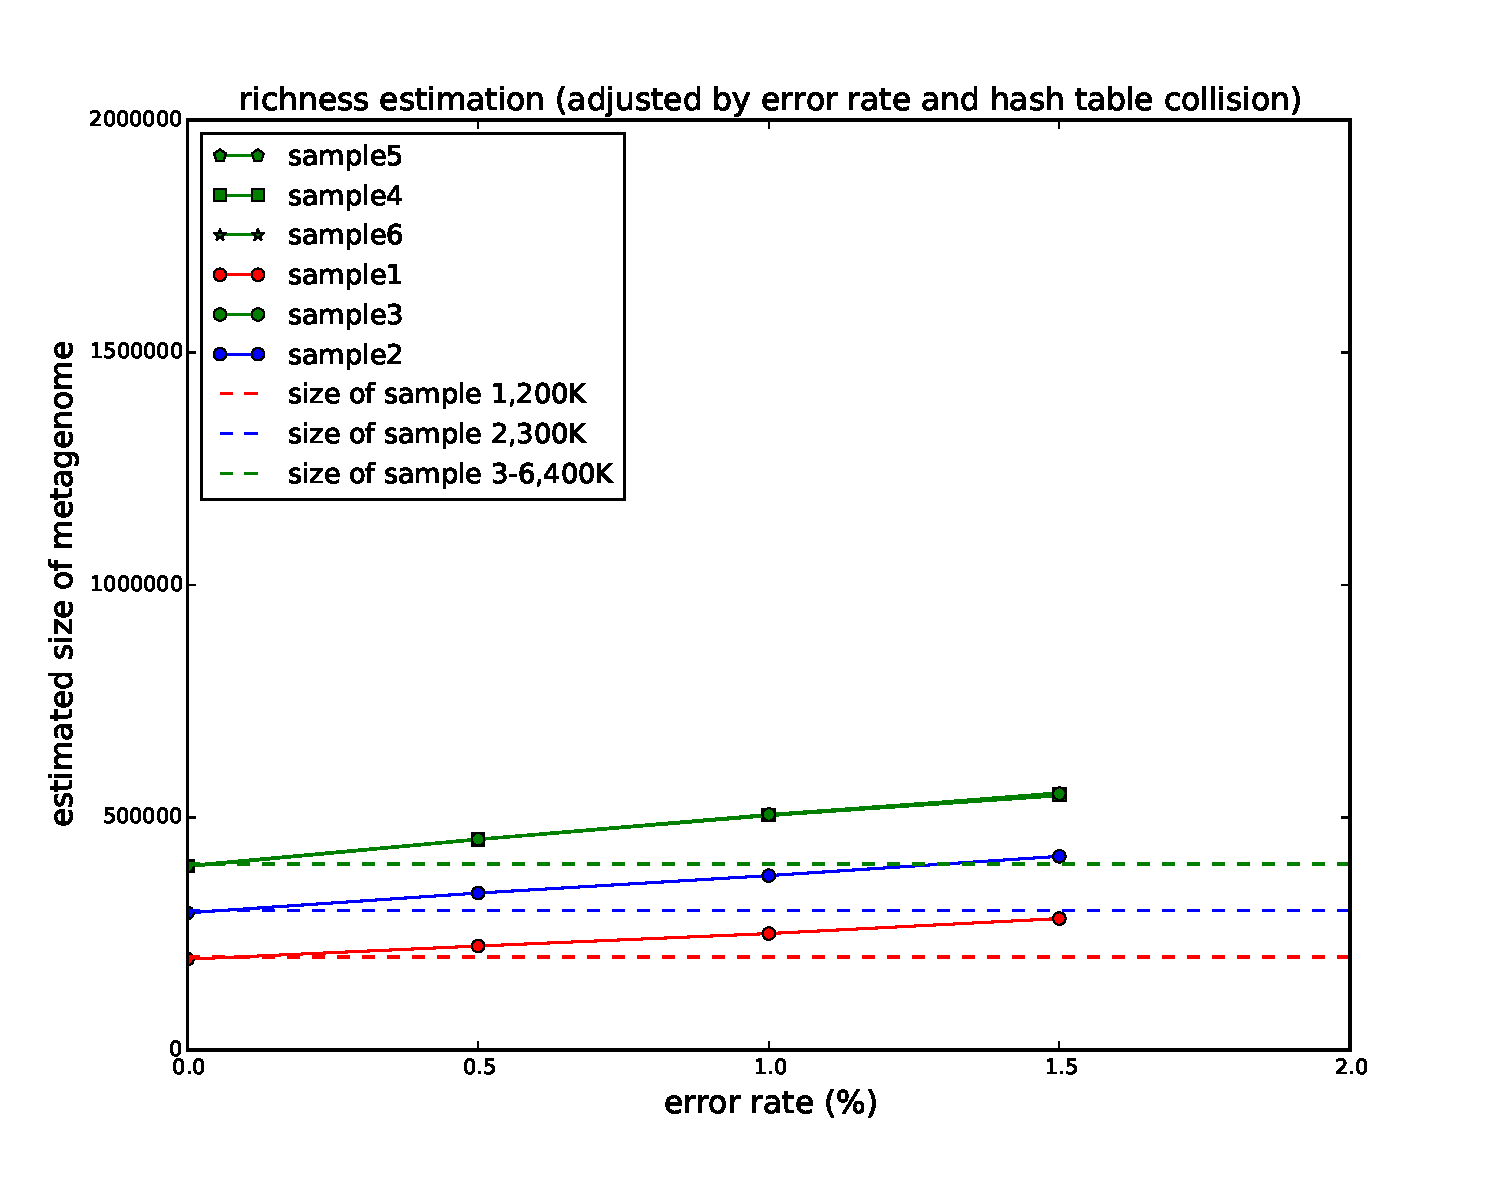
\includegraphics[width=4in]{./figures/alpha_by_error_full_adjust.pdf}}
\caption{\bf Richness estimation using IGS method adjusted by sequencing error
rate and false positive rate of bloom filter}
\label{fig:IGS_richness_adjustment}
\end{figure}


\subsection{the effect of sequencing depth to the accuracy of IGS method}


We have shown that the IGS method can generate good result from relatively
high coverage data (like 10X). It is expected that the higher the coverage
of data is, the more accurate analysis we can conduct. However for many 
metagenomics project,especially about the environmental samples, it is difficult
to yield high enough sequencing depth. We investigated the effect of 
sequencing depth to the accuracy of the IGS method.


Figure \ref{fig:IGS_correlation_coverage} shows how well the matrix 
calculated from data set with variable coverage can 
reflect the real relationship between samples. It is as expected that 
higher coverage data will yield better/more accurate distance matrix.
Note even with a coverage as low as 0.1, the correlation is 0.89. 
This can  give us the hint about how reliable the result will be if 
we only use a small proportion of data from a large metagenomic data set.
So the beta diversity analysis using IGS method not only is less prone to
sequencing error, but also less prone to sequencing depth.


% what if lower?? 0.01 for soil ?? 
% relationship between ordination/clustering and correlation??? 0.89, is it good enough to do ordination/clustering?


\begin{figure}[!ht]
 \centerline{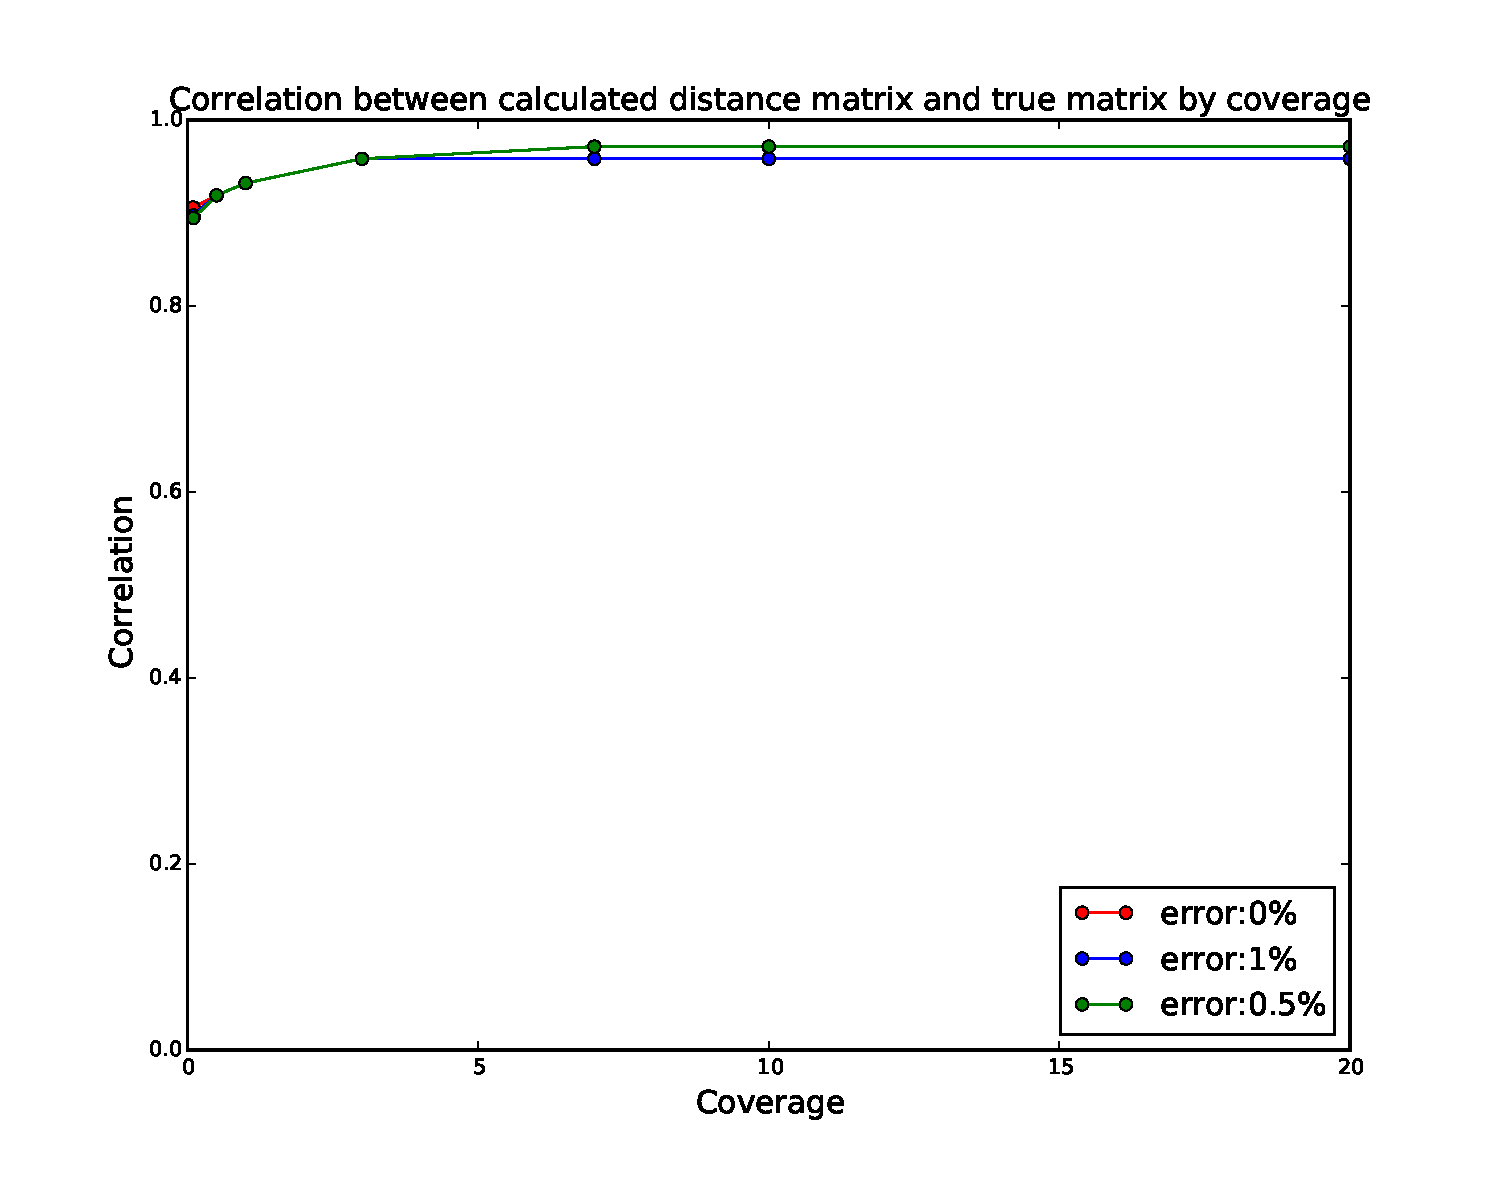
\includegraphics[width=4in]{./figures/beta_by_coverage.pdf}}
\caption{\bf Correlation between calculated distance matrix and true matrix from different dat sets with different sequencing depth}
\label{fig:IGS_correlation_coverage}
\end{figure}



Figure \ref{fig:alpha_by_coverage_0e} \ref{fig:alpha_by_coverage_0005e} \ref{fig:alpha_by_coverage_001e} 
shows the estimated genome size 
from data sets with variable coverage with different error rate.
It's interesting that the estimated genome size is very high with extremely low 
coverage. This is probably due to the limit of statistical model to estimate
the total size of information with limited observed information.
After all, only a small proportion of the genomes in the sample is covered by
reads and be observed. 

We can see the pattern again here that higher error rate will influence the accuracy
of genome size estimation,especially when the coverage is low. However for error rate
from 0\% to 1\%, as long as the coverage is higher than 1X, the estimation of 
genome size starts to be stable. 
It is important to point that even though the absolute value of estimated 
genome size may be overestimated. The relative relationship between samples 
are reliable, as shown in the figures. Sample3,4,5,6 all have 4 species, while 
sample 2 has 3 species, and sample 1 has 2 species. 
They can be separately effectively.

The estimation of genome size does not increase much with increasing coverage, 
even for the data set with error rate as 1\%. This proves that the adjustment method discussed
previously does eliminate most of the bad effect of sequencing errors. 
That being said, it is still beneficial to do some preprocessing to the data
to reduce the error rate. If only the error rate can reduce from 1\% to 0.5\%, the 
estimated size of genome will be more accurate. This again demonstrates the importance of
the streaming method doing error profile analysis discussed in chapter 4 above.

\begin{figure}[!ht]
 \centerline{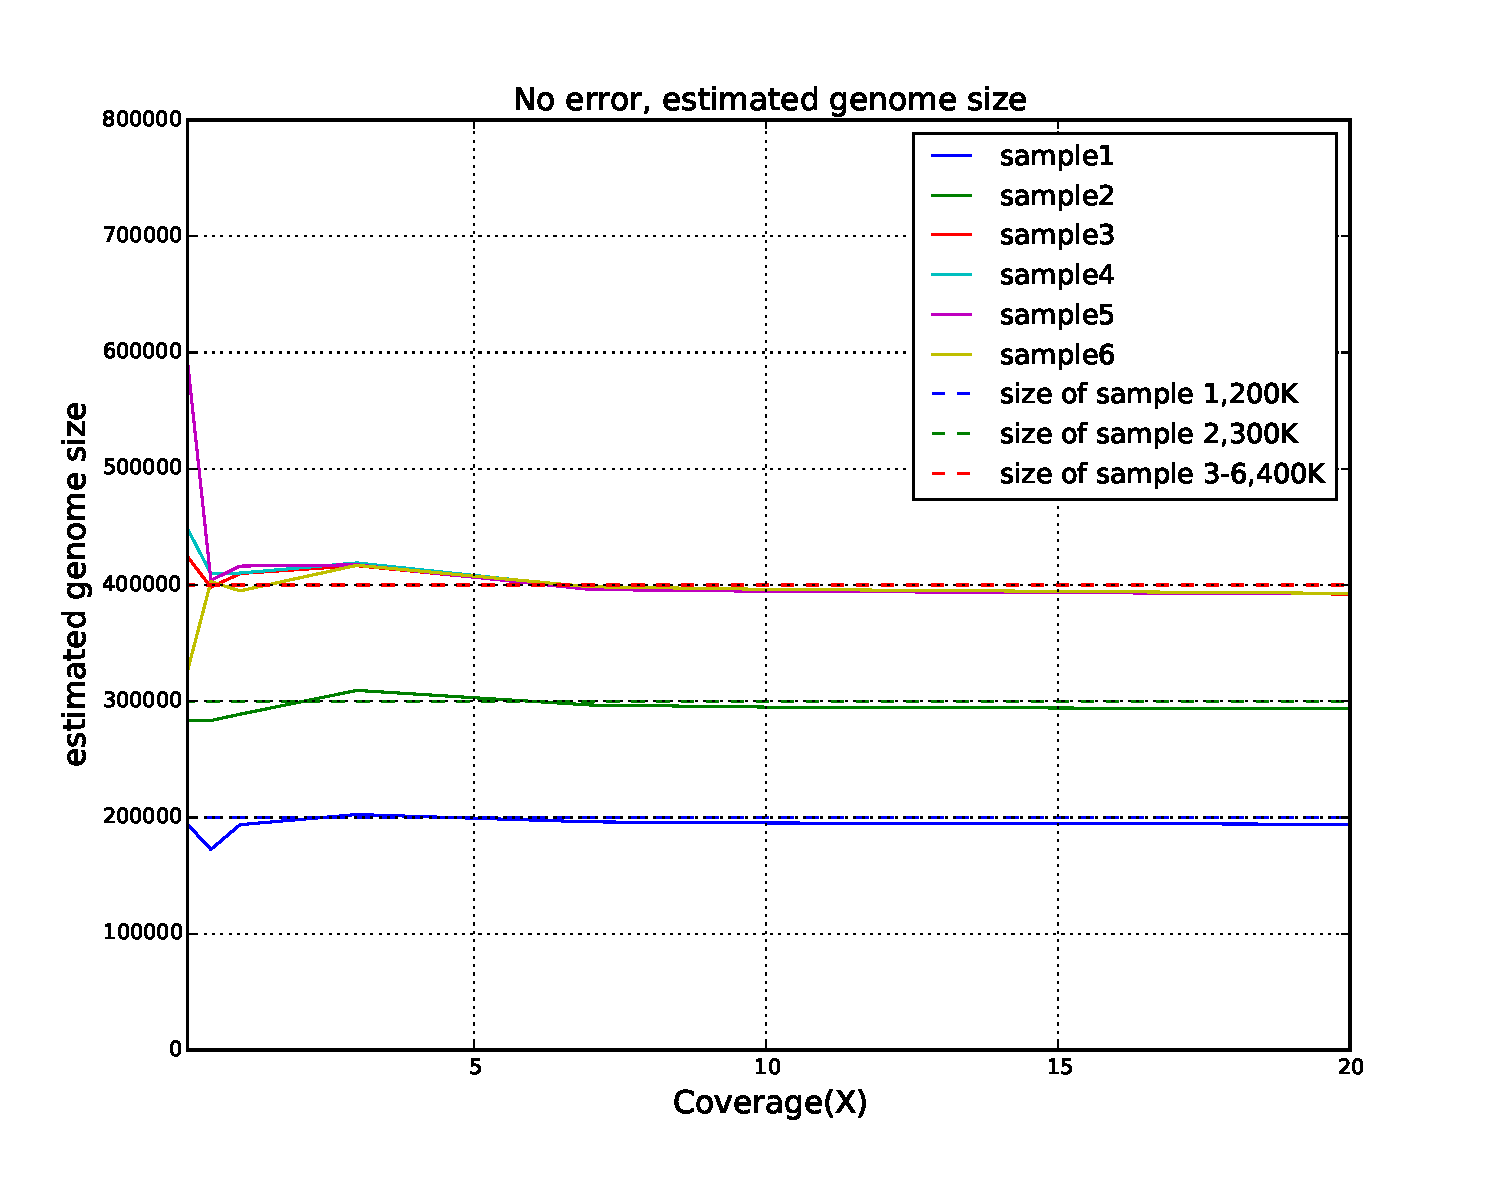
\includegraphics[width=4in]{./figures/alpha_by_coverage_0e.pdf}}
\caption{\bf estimated genome size from data sets with variable coverage, no error rate}
\label{fig:alpha_by_coverage_0e}
\end{figure}

\begin{figure}[!ht]
 \centerline{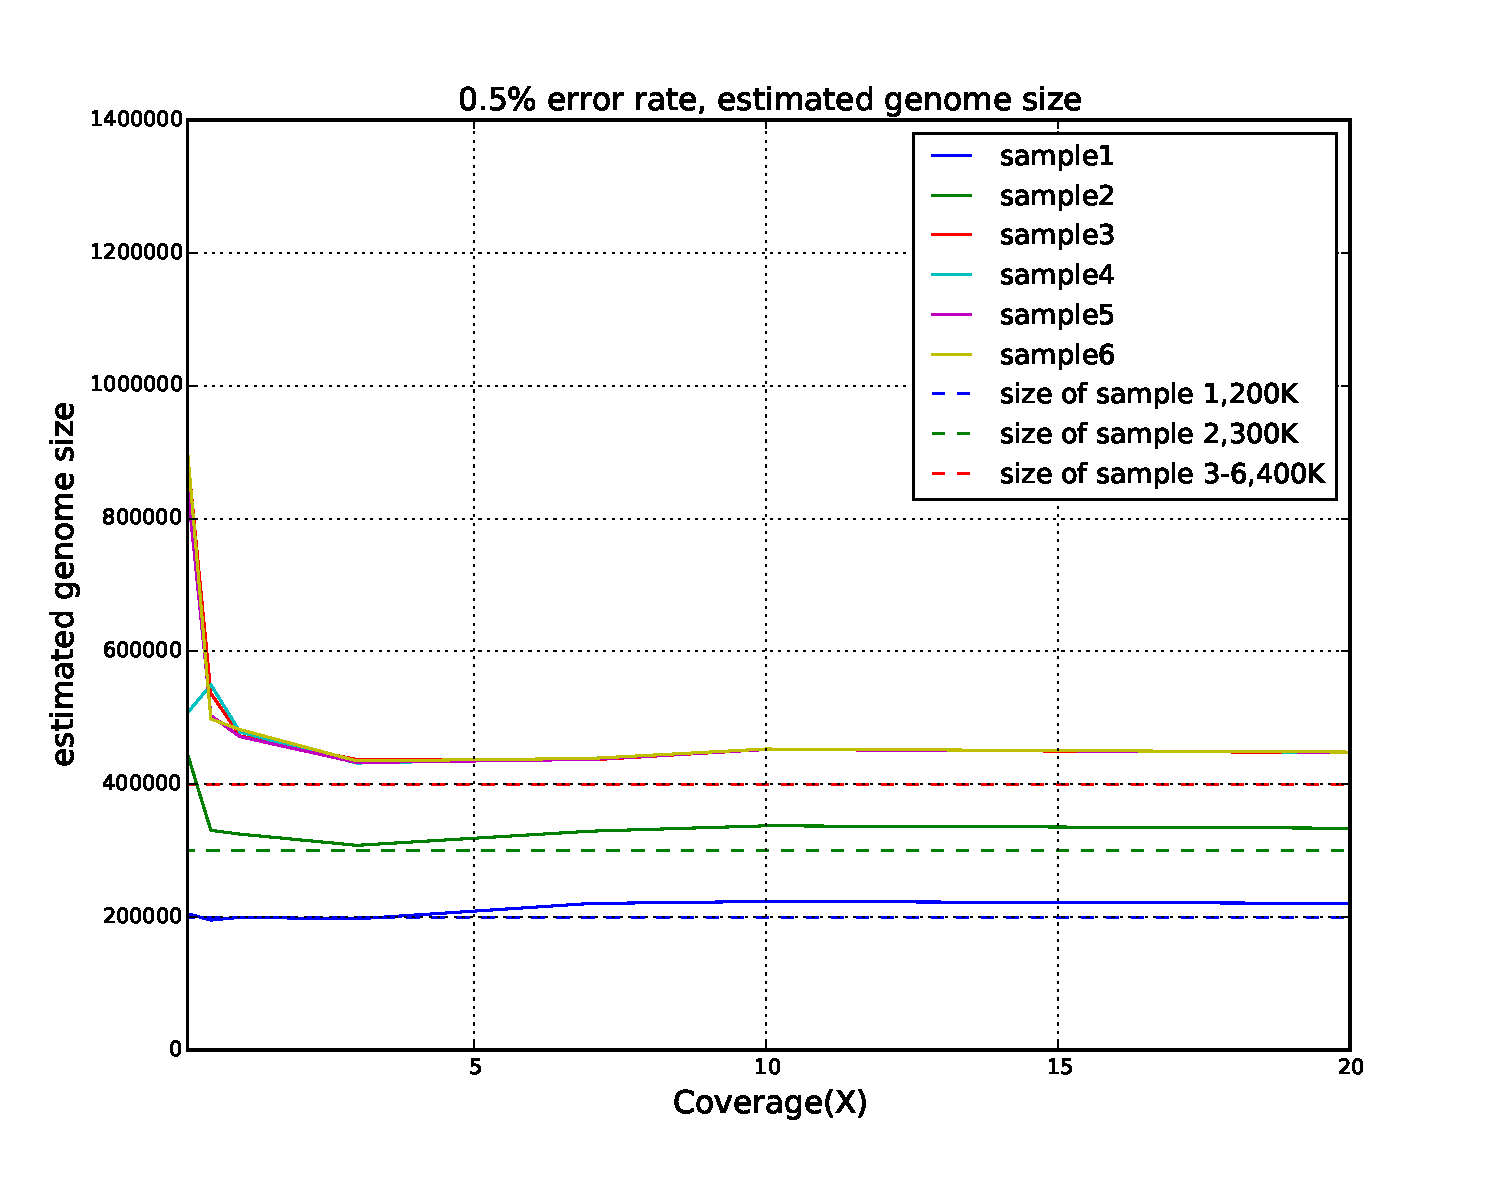
\includegraphics[width=4in]{./figures/alpha_by_coverage_0005e.pdf}}
\caption{\bf estimated genome size from data sets with variable coverage, no error rate}
\label{fig:alpha_by_coverage_0005e}
\end{figure}

\begin{figure}[!ht]
 \centerline{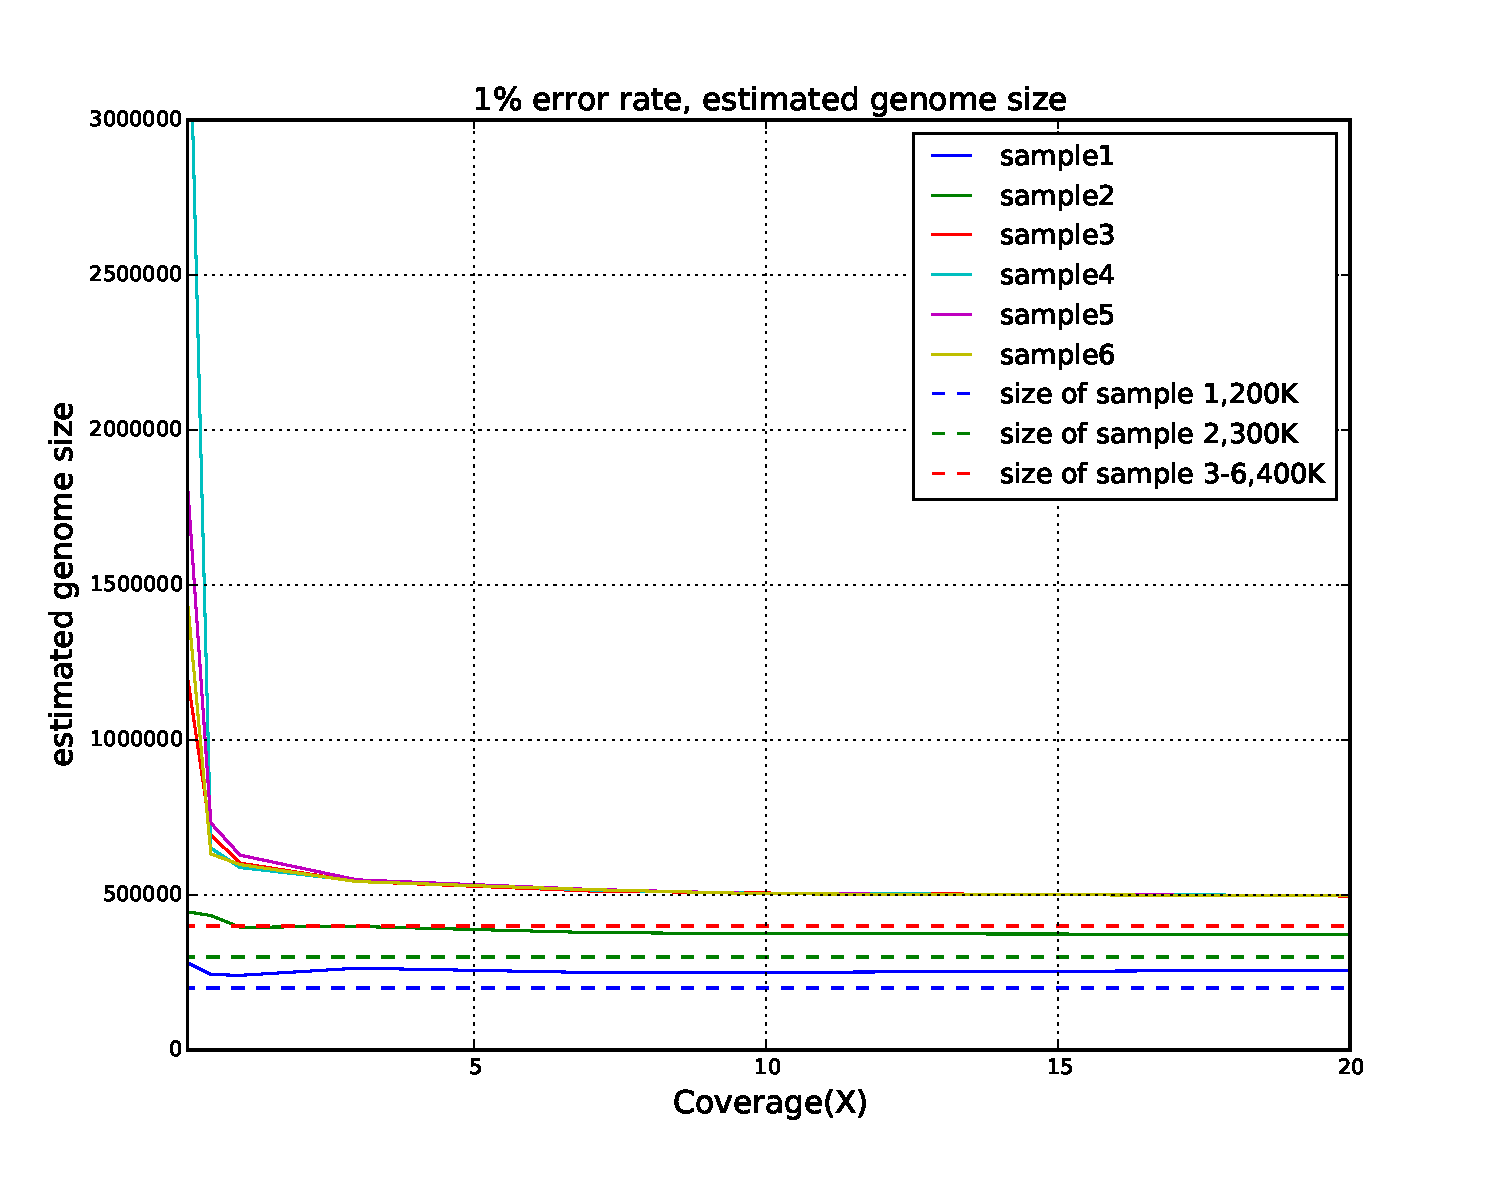
\includegraphics[width=4in]{./figures/alpha_by_coverage_001e.pdf}}
\caption{\bf estimated genome size from data sets with variable coverage, no error rate}
\label{fig:alpha_by_coverage_001e}
\end{figure}


\subsection{Compare IGS method to Commet in beta diversity analysis}


Next we test how well the matrix calculated by various methods can reflect the
real relationship between samples. 
The simulated data set with sequencing depth as 0.1X and 10X, with 
sequencing error as 1\% and without sequencing error was used in this experiment.
This data set has the same species composition as that used in other experiment previously.

As shown in Figure \ref{fig:compare_commet}, firstly, for 
all data sets, the matrix from IGS method has a higher 
correlation to golden standard than that from Comet.  As expected, 
the matrix from data sets with sequencing error has a lower correlation 
than that from error-free
data sets. Comet is more prone to sequencing error rate, compared to 
IGS method, for high coverage data or low coverage data.
Also higher coverage will yield more accurate matrix, which is not surprising.

In the experiment below with real metagenomic dataset, we will see more evidence
that IGS method has better performance than other metagenome comparing methods.

\begin{figure}[!ht]
 \centerline{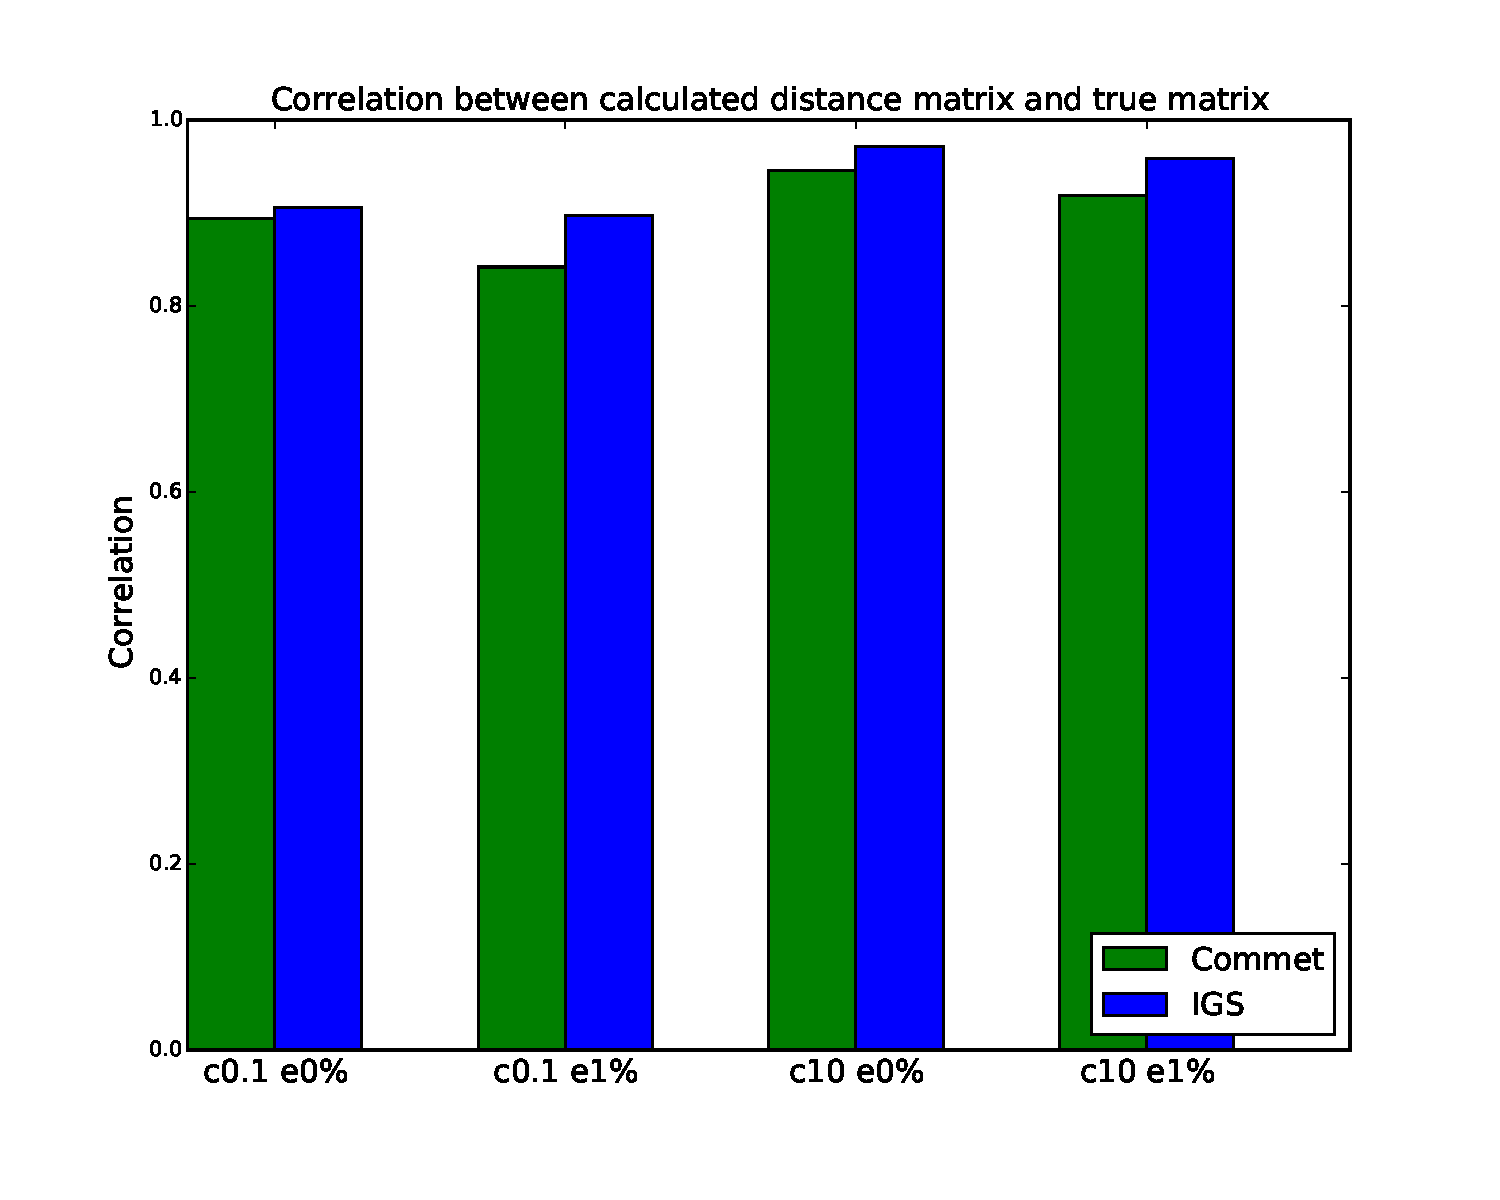
\includegraphics[width=4in]{./figures/compare_commet.pdf}}
\caption{\bf Correlation between calculated distance matrix and true matrix from different data sets and using different methods}
\label{fig:compare_commet}
\end{figure}

\subsection{The IGS method can provide a whole framework to do alpha or 
beta diversity, with good versatility.}

From the testing using simulated data sets shown here, we are confident that 
our IGS method works well and can give reliable results from data sets with 
error and low sequencing depth.

The IGS method can provide a whole framework to do alpha or beta diversity. 
Here we tested beta diversity using only Bray-Curtis metric and alpha 
diversity on richness only. Actually any metric can be applied to the 
IGS-by-samples table, just as OTU-by-samples table, 
no matter it is abundance-based or incidence-based, about richness or about 
evenness.

Compareads(Commet) based on reads overlap between samples can get a matrix 
reflecting the real relationship between samples but it is stuck with one 
metric, which is based on the percentage of overlap reads between samples. 
This metric is like Bray-Curtis , but not exactly the same.


\section{Applying IGS method to real metagenome data sets}

Having shown that the IGS method delivered good results about microbial diversity 
from simulated synthetic data sets, 
we will now evaluate the novel method on several published metagenomic 
datasets, with samples 
from ocean, human microbiome and soil. For the ocean sample and human microbiome 
data sets, we will compare the result from IGS method
with that from original publication. For soil sample, since there is no other 
diversity analysis that has been conducted
to these data sets, we will show the result we got from IGS and try to 
interpret the ecological meaning.


\subsection{GOS data sets: Sorcerer II Global Ocean Sampling Expedition}

We tested the IGS method on a famous public dataset from the Sorcerer II 
Global Ocean Sampling expedition.
During the expedition, 44 water samples were collected from different locations across
Atlantic Ocean and Pacific Ocean and were sequenced using Sanger technology. 
The whole dataset is composed of XXXX reads, out of 44 samples.
A whole metagenomic comparison of the samples has been done
using a sequence alignment method in original research. 

The IGS method took XX hours on a XXX hardware to generate the dissimilarity 
matrix of the samples. After clustering, 
Figure \ref{fig:GOS-beta} shows that, consistently with the original study, 
the samples are clustered according to their 
geographical origin. The group with yellow color contains samples from 
Tropical- Galapogas. The group with light purple color
contains samples from Tropical -Open Ocean. The group with dark purple 
color contains samples from Sargasso. The group 
with green color contains samples from Temperate. 

If we compare the cluster we got from IGS method with the cluster in original 
study, we can see the IGS method yield a
cluster with better resolution and accuracy than the method used in original 
study. For example, in original study,
sample 14,21 and 22 from Tropical - Galapogas are separated from other 
Tropical- Galapagos samples, while in Figure \ref{fig:GOS-beta} 
they are grouped together. Also, samples 00a,00b,00c,00d, obviously from the 
same location, are grouped together in our result,while
in original research, sample 00a is separated from the other three samples.

Compared with the cluster by Compareads, our method is comparable, with some 
distinct differences. For example, sample 16 is clustered together with 15,17,
18,19 in our result, but in the result by Compareads, sample 16 is clustered 
with 23,26 inaccurately, considering the geographical origin.

Next we used IGS method to analyze the alpha diversity.
Figure \ref{fig:GOS-rarefaction} shows the rarefaction curve of IGSs of the samples.
As expected, we can not see the saturation,which means the sequencing data 
set is still far from having enough coverage. 
Because the data sets for different samples have dramatically different sizes, 
we estimated the total number of IGSs using Chao1 estimator with limited 
number of reads in each sample(50000) to make sure the smallest data set 
has enough reads for comparison, as shown in Figure \ref{fig:GOS-chao1} .

It is obvious that the richness of samples is related to the geographical 
origin. The sample from tropical area has a higher richness than
the samples from northern area. The relationship between samples is 
consistent to the cluster in beta diversity analysis shown above.

As discussed in the section above about alpha diversity analysis 
to synthetic data, such number of total IGSs may over-estimated but
the relative relationship between samples on richness should be reliable.

(This is not discussed in original research of GOS)

\begin{figure}[!ht]
 \centerline{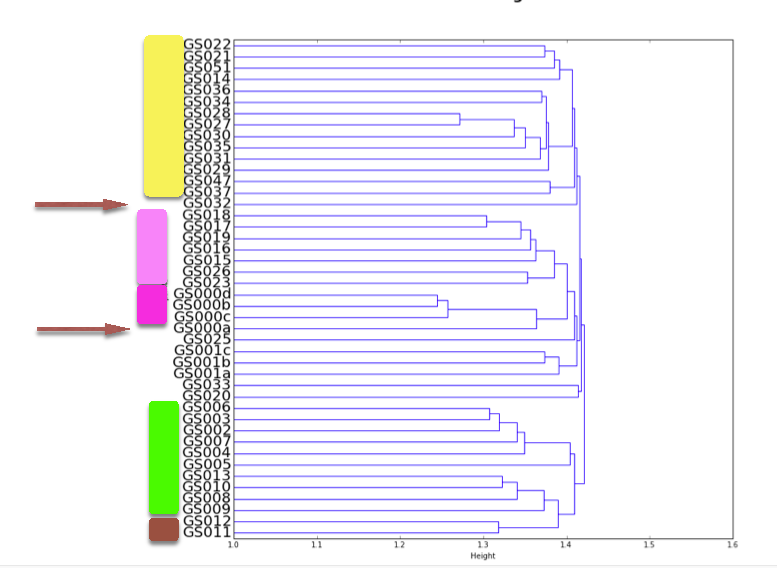
\includegraphics[width=7in]{./figures/GOS_cluster.png}}
\caption{\bf cluster of GOS samples using IGS method}
\label{fig:GOS-beta}
\end{figure}

\begin{figure}[!ht]
 \centerline{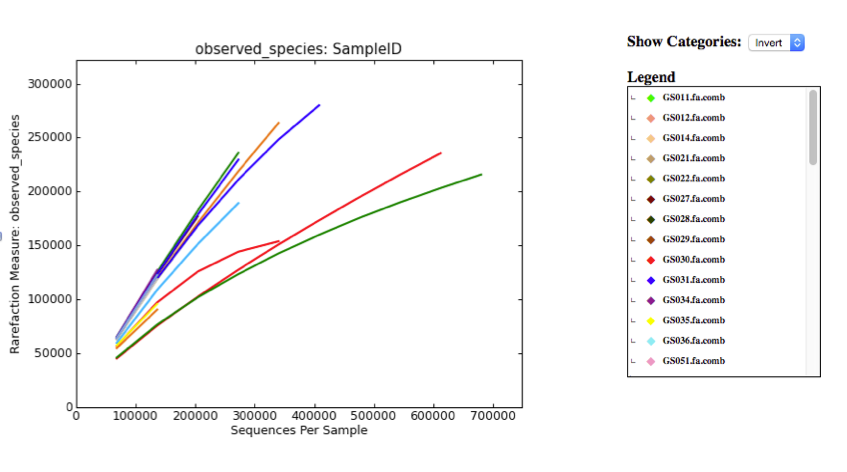
\includegraphics[width=7in]{./figures/GOS_observed.png}}
\caption{\bf Rarefaction curve of IGSs of the GOS samples}
\label{fig:GOS-rarefaction}
\end{figure}

\begin{figure}[!ht]
 \centerline{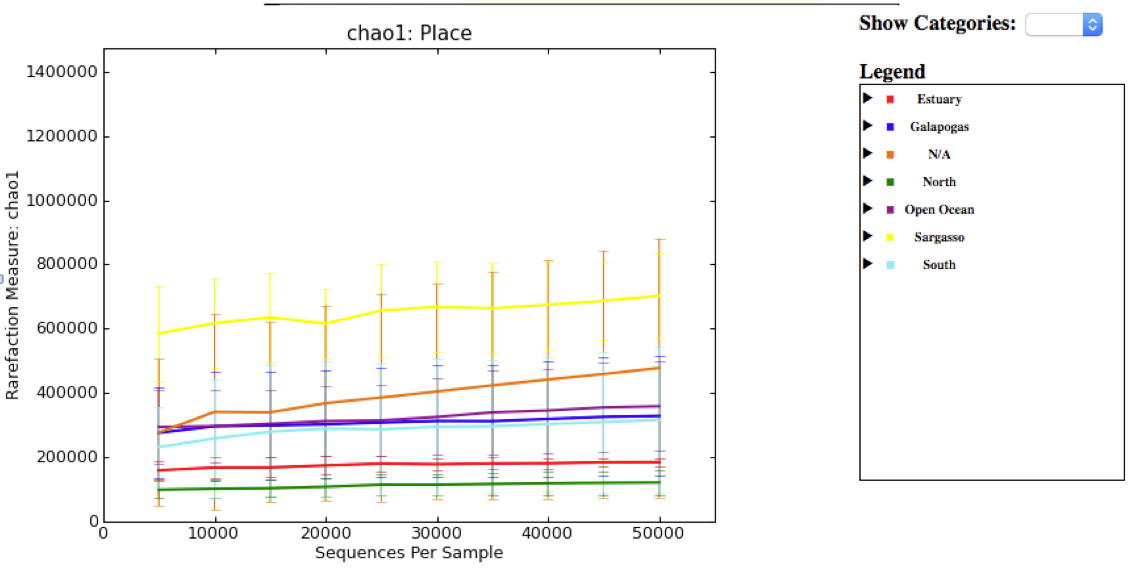
\includegraphics[width=7in]{./figures/GOS_chao.png}}
\caption{\bf Estimated number of IGSs of the GOS samples}
\label{fig:GOS-chao1}
\end{figure}


% result not good, remove it?
%\subsection{MetHit Human Gut metagenomics data set}


\subsection{HMP metagenomics data set}
% now have alpha and beta, smallest samples
% full sample 110 .... good for binning?

We tested IGS method on 12 HMP(Human Microbiome Project) samples from 
different body parts like skin, oral or vaginal. 
Principal component analysis(Figure \ref{fig:HMP_beta}) shows the samples are 
separated well by the body parts where they are collected. (P value: XX)

Rarefaction curve and estimated number of IGSs show that the richness of 
samples is related to the body part where they are collected. The 
oral samples have higher richness than skin or vaginal samples, 
which is consistent  to other research. \cite{Human-Microbiome-Project-Consortium:2012aa}



\begin{figure}[!ht]
 \centerline{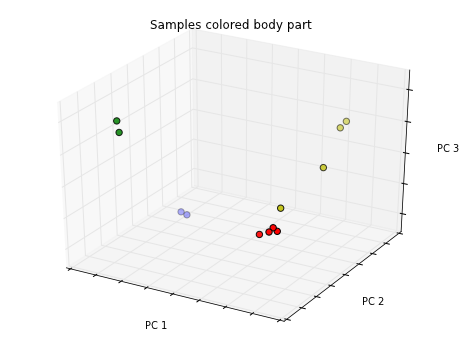
\includegraphics[width=4in]{./figures/HMP_beta.png}}
\caption{\bf PCoA of HMP, red: anterior nares- skin, green: throat -oral, blue: buccal mucosa -oral, orange: 
posterior fornix -vaginal}
\label{fig:HMP_beta}
\end{figure}

\begin{figure}[!ht]
 \centerline{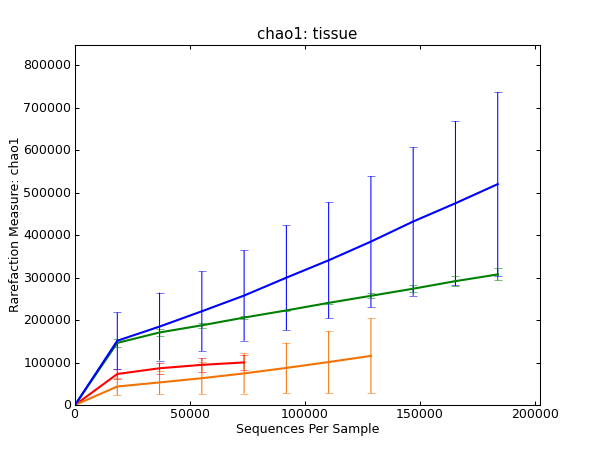
\includegraphics[width=4in]{./figures/HMP_alpha.png}}
\caption{\bf alpha diversity of HMP: estimation of metagenome size of HMP samples,
red: anterior nares- skin, green: throat -oral, blue: buccal mucosa -oral, orange: 
posterior fornix -vaginal}
\label{fig:HMP_alpha}
\end{figure}





% ARMO subset 1m, Gpgc only 1m/2m subset, scalable??
\subsection{GPGC - Great Prairie Soil Metagenome Grand Challenge}

Having tested the IGS method on two relatively smaller metagenomic data sets, 
we will now use it to analyze 
a larger data set from soil samples collected from fields with different treatments and
different locations across the great prairie region in the US. 
(Table \ref{table:gpgc}). 


%new GPGC has better understanding??

% should be enough??
As discussed above with simulated data sets, using reads data sets with lower sequencing coverage will reduce
the accuracy of the analysis. But as shown in Figure \ref{fig:IGS_correlation_coverage}, with sequencing depth
as 0.1x, the calculated distance matrix using IGS method still has a reasonably high correlation with golden standard
distance matrix. So we can use subset of a large data set to acquire the diversity information, with the trade-off of
lower accuracy. 

For the GPGC datasets, we made a subset with 2 million reads from each sample 
and conducted the diversity analysis
using IGS method. 

Principal component analysis(Figure \ref{fig:GPGC_beta}) shows the samples are 
separated well by location where they are collected. (P value: XX)
This proves that the geographical origin plays a more important part in 
determining the similarity of genomic composition of samples, compared to 
different treatments.

Figure \ref{fig:GPGC-alpha} shows the rarefaction curve and estimated number 
of IGSs of the samples. Basically the ``corn'' and ``switchgrass'' samples
have higher richness than ``restored'' and ``prairie'' samples. This observation 
that cultivation increases the richness of soil 
is consistent with the intermediate disturbance hypothesis.(citation) The disturbance 
from treatment like cultivation opens more niches and the stable 
community like prairie eliminates some populations by the principle of 
competitive exclusion. . 

Its harder to explain the rank by state. 
The Kansas site experiences more drought stress and higher temps. 
The Iowa and 
Wisconsin sites experience more cold, especially freezing conditions arresting 
their biology for 3-4 months, but the freeze-thaw cycles also kill off 
some each cycle, which is similar to intermediate disturbance. With new 
growth each spring, this new growth would be the fast growers with 
less diverse. Why Iowa is the least diverse is still difficult to explain for now.

 From the alpha diversity, we also have a rough estimation of the  total 
 size of metagenome in Iowa soil, which is about 540G basepairs. This 
 proves the high complexity of soil sample and we still need more sequencing 
 effort to achieve a reasonable high coverage.
 

\begin{figure}[!ht]
 \centerline{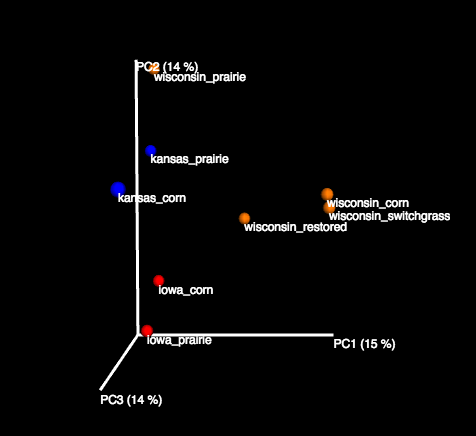
\includegraphics[width=4in]{./figures/GPGC_old_subset1M.png}}
\caption{\bf PCoA  of GPGC samples}
\label{fig:GPGC_beta}
\end{figure}



\begin{figure}[!ht]
 \centerline{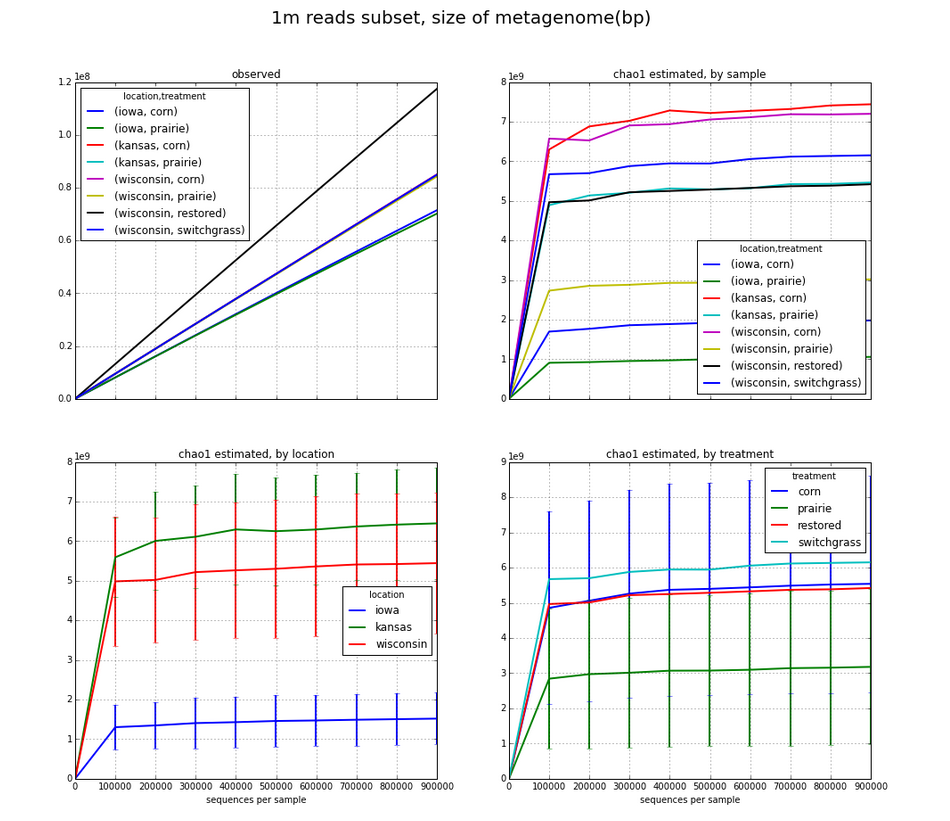
\includegraphics[width=7in]{./figures/GPGC_1m_old.png}}
\caption{\bf alpha diversity of GPGC samples}
\label{fig:GPGC-alpha}
\end{figure}



%\section{iterated diversity analysis}

%As we load more reads, we will see the separation more clearly. 

%simulated data sets. 

\subsection{more soil metagenomic samples}

Additionally we test the IGS method on two other unpublished data sets. 
One is a series of soil samples
collected from KBS with different treatment. Figure \ref{fig:KBS_beta}
shows the IGS method can separate
the samples by treatment well. 

The other data set is a series of soil samples from Amazon rainforest. 
The samples are separated well
by the treatment. (Figure \ref{fig:ARMO_beta} ) It is also obvious 
that samples from forest have 
lower richness than prairie.  (Figure \ref{fig:ARMO_alpha})




\begin{figure}[!ht]
 \centerline{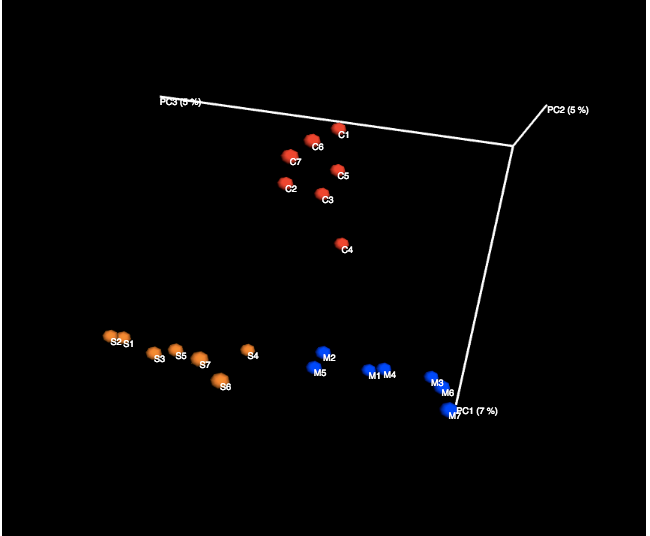
\includegraphics[width=4in]{./figures/IGS_KBS_beta.png}}
\caption{\bf PCoA of soil samples collected from KBS}
\label{fig:KBS_beta}
\end{figure}

\begin{figure}[!ht]
 \centerline{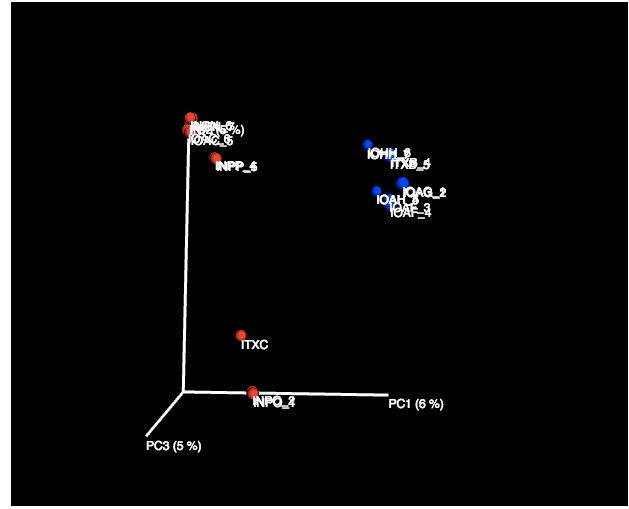
\includegraphics[width=4in]{./figures/IGS_ARMO_beta.png}}
\caption{\bf PCoA of soil samples collected from Amazon rainforest}
\label{fig:ARMO_beta}
\end{figure}

\begin{figure}[!ht]
 \centerline{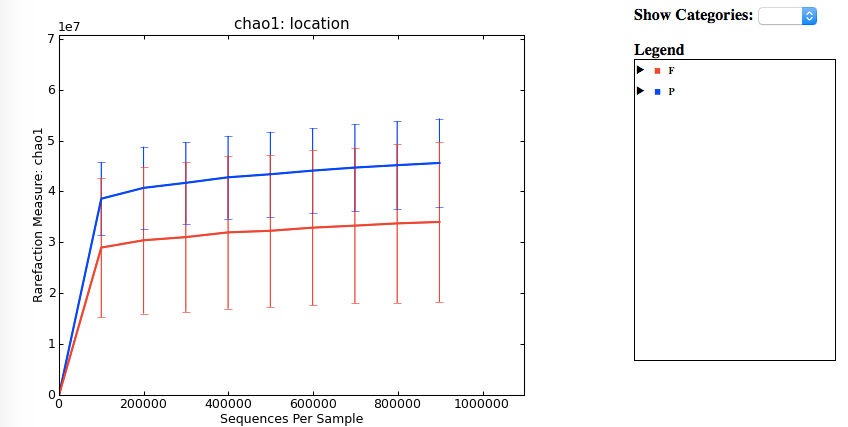
\includegraphics[width=7in]{./figures/IGS_ARMO_alpha.png}}
\caption{\bf PCoA of soil samples collected from Amazon rainforest}
\label{fig:ARMO_alpha}
\end{figure}


\section{Data}


\subsection{Code availability}
The algorithms of the IGS based diversity analysis are implemented 
 in the khmer software
package, written in C++ and Python, available at github.com/ged-lab/khmer/.
 khmer also relies on the screed package for loading
sequences, available at \\
github.com/ged-lab/screed/.
khmer and screed are Copyright (c) 2010 Michigan State University, and are free
software available for distribution, modification, and redistribution under the
BSD license.

The code and detailed instruction used to generate all the results in this 
chapter is available at
http://github.com/ged-lab/2013-diversity/. 


\subsection{Simulated sequencing reads of e.coli}




\begin{table}[h]
\caption{GPGC Data sets}
\label{my-label}
\begin{tabular}{|l|l|l|l|l|}
\hline
sample & \# of reads & size of .gz file & \# of bps & ave. length \\ \hline
iowa corn & 1514290825 & 46G & 144202427079 & 95.2 \\ \hline
iowa prairie & 2597093273 & 74G & 226815059143 & 87.3 \\ \hline
kansas\_corn & 2029883371 & 66G & 206933829048 & 101.9 \\ \hline
kansas\_prairie & 4987358734 & 145G & 499387223498 & 100.3 \\ \hline
wisconsin\_corn & 1616440116 & 51G & 162257698471 & 100.4 \\ \hline
wisconsin\_prairie & 1653557590 & 53G & 166467901724 & 100.7 \\ \hline
wisconsin\_restored & 226830595 & 11G & 34241520930 & 151.0 \\ \hline
wisconsin\_switchgrass & 310966735 & 13G & 40259619921 & 129.5 \\ \hline
\end{tabular}
\label{table:gpgc}
\end{table}


%check the reads coverage in the sample where it is from
%
%\section{de bruijn graph mapping}
%
%check the reads coverage in another sample
%
%\section{IGS-based diversity analysis}
%


\chapter{Conclusion}

%Advantage:

%not only HMP, high depth, data
%but also low depth data, like soil metagenomics, which is impossible to use traditional method 


We have developed a novel statistical framework to enable microbial diversity
 analysis using whole genome shotgun metagenomic reads data without the
requirement of assembly, binning, reference or annotation. This dissertation
covers an overview of existing approaches of performing microbial diversity analysis
 of metagenomic samples, especially based on the concept of OTU, including the
steps in the procedure, like contigs binning, statistical
analysis of OTU abundance information to estimate the microbial diversity. Next
the statistical framework based on the novel concept of IGS was discussed. As
the foundation of the framework, we described a novel method to count k-mers
efficiently and a scalable approach to retrieve the coverage of a read in a 
data set based on efficient and online k-mer counting. We also introduced the
applications of this approach in reducing the redundancy of metagenomic reads
dataset and analyzing sequencing error, which is beneficial to other tasks 
in metagenomic data analysis, like
assembly or error trimming. Finally, we discussed how we developed the concept 
of IGS based on the methods of efficient k-mer counting and digital
normalization discussed before.  
The application of IGS to analyze microbial diversity of metagenomic data sets 
was discussed and the performance of the IGS method on simulated data sets and
real data sets were demonstrated in the final chapter. In this chapter, we
summarize how the novel statistical framework based on IGS makes a difference to
 the diversity analysis in current microbial ecology research. 
Finally some directions of future work will be discussed.

  

\section{Summary}

Diversity analysis is a key part of the microbial ecology research, like of
macroorganism ecology. However due to the obscure definition of the term
"species" in microbial ecology, we can virtually never measure the diversity of
species directly, rather we use other taxonomic concepts like operational
taxonomic unit (OTU) to evaluate the diversity of microbial community, instead
of species. 16S rRNA sequencing reads may be classified into different OTUs.
Shotgun whole genome sequencing reads can also be classified into OTUs. But
most, if not all the existing methods based on the concept of OTU rely heavily on  
preprocessing of original reads data in some way like assembly or external 
information like reference sequences for annotation. Both of the prerequisites
are not satisfied for many metagenomic projects. For some low coverage
metagenomic reads data, assembly can only extract partial information about the
species with higher abundance. It is common that only a small proportion of
reads can be used in assembly especially in a complex environmental sample. \cite{Howe2012} The reference sequence database is far from
completion especially for microbes in environmental samples from soil or sea water.
Thus applying these methods can only get a partial picture of diversity of
the microbial community the metagenomic sequencing data covers. 

The IGS based
method discussed in this dissertation offers a brand new framework that
bypasses the difficult tasks like assembly, binning, or annotation without the
requirement of reference sequence database. It can take advantage of all the 
information in the metagenomic reads data and gain a full picture of the
diversity of the microbial community. The fact that this is a whole new
framework with the concept of IGS replacing OTU as the taxonomic unit to
analyze diversity means that this framework can be used to do all possible
diversity analysis that OTU-based framework can do. This is a more thorough
solution than many other methods that are developed to solve some specific
problems in the field of diversity analysis. For example, there are several
methods developed to estimate the richness of a metagenomic sample or the size 
of metagenome \cite{Rodriguez-R2014}. Our IGS based framework can not only
estimate the richness or size of metagenome as shown in the section above, but
also it can estimate the evenness or species abundance distribution of a
metagenomic sample, which is also an important aspect of alpha diversity
analysis. For beta diversity or compositional similarity analysis between
metagenomic samples, there are several methods developed to compare metagenomic
samples based on reads mapping or counting shared reads \cite{Rodriguez-R:2013aa}.
But basically they only estimate abundance-based similarity, similar to
the Bray-Curtis indices used in the experiment discussed in the section above.
Actually what is not shown in the results in the text here is that the 
IGS-based framework can also be used to estimate incidence-based similarity, if
such information is interesting to the researcher.

Besides the advantage of the IGS based framework that it has a broad
application with its versatile potentials, this framework is also efficient and
highly scalable to handle extremely large metagenomic sequencing data
sets. We have discussed the efficiency of the novel k-mer counting method and
the following method of digital normalization, with the ability to retrieve the
coverage of a read accurately and efficiently. We also did thorough analysis
to the effect of the size of used data structure to the accuracy. We can take
advantage of the probabilistic characteristics of the data structure to make a
trade-off between expected analysis accuracy and expected usage of
computational power. In this way, we make the analysis highly scalable to
the increasing size of metagenomic sequencing data.  

Also, for the purpose of estimating microbial diversity of metagenomic samples,
we analyzed the effect of sequencing depth to the accuracy of the estimation.
It is obvious and expected that using more reads data with higher sequencing
depth increases the accuracy of such diversity estimation. Especially for beta
diversity or similarity analysis between samples, reads data with relatively
low sequencing depth can still get decent results, as shown in the experiment
with synthetic data and real soil data sets. For alpha diversity like richness
estimation, using reads data with lower sequencing depth gets the estimation
more distant from the real number, but although the absolute value of such species
richness of a sample is not accurate, the relative comparison of species
richness between samples are less prone to smaller reads data with lower
sequencing depth. These analysis and observation convince that for specific
purpose, only a subset of the large metagenomic reads data can be enough to
achieve reasonably satisfying result. Under certain circumstance, this feature
is quite helpful and can reduce the computational expense dramatically. 


\section{Future Work}


Though this dissertation demonstrated the performance of the new approach to 
analyze microbial diversity
using whole genome shotgun sequencing data without the requirement of assembly,
binning, or annotation, there is still plenty of room for improvement.  

Basically the question that the IGS based method is developed to answer is how many
species there are in the sample or how similar the samples are between each
other, mostly focusing on the quantitative aspect. Admittedy these are 
important questions the microbial ecologists want to answer, they are also
curious about the qualitative questions, like if two samples are different, what
the stuffs that make the difference are, and what  the function of
those stuffs is.\cite{Xu2014}  A natural expansion of the IGS based framework will lead to
answer questions like this. 

Now we have an efficient and scalable approach to get the coverage of a read in
a sample, it is straightforward to extract the reads according to its coverage
profile across samples so we can get a subset of reads that have specific
properties, like the reads that are common in all samples. In this way we
may collect these "common" reads from samples together and try to co-assemble
them since now they should have higher coverage. Or we can get a subset of
reads that are common in a group of samples but do not exist in another group
of samples, like the samples from patients and healthy persons. These
"signature" reads may offer important insights to understand what happens
to the microbial community while the environment changes. Admittedly these
kinds of "extraction" can be implemented using other methods like reads 
alignment method. But they may not be as efficient and scalable as the IGS
based method, especially for extremely large metagenomic data.


One advantage of the IGS based method is that binning is not required in this
procedure. Firstly, traditionally binning is used to classify contigs after some
kinds of assembly effort. The similarity based binning method relies on
sequence alignment, which is not efficient, especially infeasible for large
metagenomic data. Also, reference sequences normally are required for
similarity based binning approach. The composition-based approach relies on the
frequency profile of sequence signatures and machine learning approach on that
profile, which is computationally expensive. 
The third approach based on coverage profile across samples was developed
recently.\cite{Imelfort2014}\cite{Alneberg2014} Although mostly often, the coverage
profile is used with the companion of composition frequency profile to classify
contigs. The assumption on which the coverage profile based binning approaches
are based on, that contigs with similar coverage profile across samples are
more likely to be from the same microbial organism, is actually similar to the
assumption on which using IGS to do beta diversity is based, that the IGSs with
similar coverage profile across samples are likely to be from the same
microbial organism. So it is promising to classify the IGSs by the coverage
profile across samples. We have already overcome the challenge of retrieving the
coverage profile efficiently based on the probabilistic data structure, while
in those coverage profile based binning approaches the coverage profile is 
normally retrieved by assembly of contigs and mapping
reads back to contigs, which both require higher coverage reads to do assembly
and are computationally expensive. 

There are two obstacles to overcome in this coverage profile based
IGS binning approach. First, with relatively small number of samples, the
resolution will be limited, since the total number of different coverage
profiles will be limited. This is probably the reason why most of those coverage
profile based contig binning methods have to integrate composition profile information
also. Second, on the other hand, if there are large number of samples, there
will be too many different coverage profiles. We can use more sophisticated
 approach to classify the coverage profiles to reduce the number of bins,
as in those coverage profile based contigs binning methods. Another approach
worthy of note is that there is a method termed partitioning developed in
our group as a divide and conquer approach to scale metagenome assembly. It can be 
considered as a binning approach also, where the reads in the same
partition are more likely to originate from the same microbial organism. We can
try to integrate the partitioning and IGS coverage profile to improve the
accuracy of the binning. In summary, this will be one of the first attempts to
do reads binning. After the IGS/reads binning,  we expect to do better assembly
 and annotation and gain more knowledge about the
function and phylogenetical information.  

We have shown that after adjustment according to sequencing error and collison
rate of the bloom filter, the estimated size of metagenome is close to real
number for synthetic data sets. But the difference between the estimation and
real number is still increasing with higher error rate, which means there is
other factor that affect the accuracy of estimation. This is worthy of further
investigation. The size estimation of metagenome is extremely important in
metagenomic data analysis and it is closely related to the estimation of
sequencing depth or how much more effort is required to gain enough sequencing
depth. As shown in the results, we are confident that the relative relationship 
between the richness of different samples is reliable from the IGS based alpha
diversity analysis. How accurate the absolute value of the richness or the size
of metagenome in a real data is requires further investigation and new  
statistical model may be needed to adapt to the abundance distribution of IGSs.    
Furthermore, any information about the richness of a sample is beneficial to
the optimal choice of parameter for digital normalization.

The analysis of the effect of sequencing depth to the accuracy of beta
diversity shows that using a relatively small subset of the whole data set may
get reasonably good result showing the separation of samples after clustering
or ordination. However how good the separation is seems to be related to the
characteristics of samples and cannot be determined easily before starting the
analysis. So a potential approach is to do such beta analysis in an iterative
way. We already know that using more data will benefit more accurate analysis or better
separation for the purpose of comparing metagenomic samples. In such
iteration procedure, how good the separation is can be monitored as more reads
are loaded into the analysis and the procedure can be stopped as long as the
pattern of the separation of samples is significant enough. This way, we may
save lots of computational cost and still have enough information about the
relationship between samples. 
 
    
    
    
    
    
    



%%%%%%%    APPENDICES    %%%%%%%%%%
%% If you wish to include one appendix, remove the "%" from the 
%% following two lines.
\renewcommand{\appname}{APPENDIX}
\appendix
\input{gloss}
%% To include several appendices, remove the only the "%"
%% in front of "\appendix".

%% In either cast to start your first appendix, which will be labeled
%% as Appendix A, just type \chapter{<appendix 1 name>}
%% and enter the text of the appendix as you would a chapter.

%%%%%%% A NOTE ABOUT APPENDICES %%%%%%%%%
%% Some appendices may be single spaced such as survey examples or letters.
%% Contact the Graduate School for details.
%% To single space an appendix first remove the % from 
%% the following two lines. 
% \end{doublespace}
% \chapter{<appendix  name>}
%% After entering the appendix remove the % from 
%% the following line
% \begin{doublespace}
%% Any text entered now will be double spaced.
\end{doublespace}

%%Bibliography 

%% A bibliography is required. By default it is called, "Bibliography"
%% You may use �Literature Cited�, �Works Cited� or �References� 
%% instead of �Bibliography� if that is the convention in your discipline. 
%% To do so, place your choice in the  empty argument 
%% of the following command and remove the "%".
\renewcommand{\bibname}{BIBLIOGRAPHY}
%% The bibliography may be made using BibTeX.
%% If it's made from scratch,
%% remove the "%" in front of "\begin{thebibliography}{???}"
%% replacing the ??? with the appropriate entry and 
%% remove the "%" in front of "\end{thebibliography}"
% \begin{thebibliography}{???}
%%  Enter the bibliography here.
% \end{thebibliography}

\bibliographystyle{abbrv}
\bibliography{dis}

\end{document}
